\PassOptionsToPackage{unicode=true}{hyperref} % options for packages loaded elsewhere
\PassOptionsToPackage{hyphens}{url}
%
\documentclass[12pt,a4paper,UTF8,twoside]{book}

\usepackage{lmodern}
\usepackage{setspace}
\setstretch{1.25}
\usepackage{amssymb,amsmath}
\usepackage{ifxetex,ifluatex}
\usepackage{fixltx2e} % provides \textsubscript
\ifnum 0\ifxetex 1\fi\ifluatex 1\fi=0 % if pdftex
  \usepackage[T1]{fontenc}
  \usepackage[utf8]{inputenc}
\else % if luatex or xelatex
  \ifxetex
    \usepackage{xltxtra,xunicode}
  \else
    \usepackage{fontspec}
  \fi
  \defaultfontfeatures{Mapping=tex-text,Scale=MatchLowercase}
  \newcommand{\euro}{€}

    \setmainfont[]{Times New Roman}
    \setsansfont[]{Arial}
    \setmonofont[Mapping=tex-ansi]{Inconsolata}
\fi

% use upquote if available, for straight quotes in verbatim environments
\IfFileExists{upquote.sty}{\usepackage{upquote}}{}
% use microtype if available
\IfFileExists{microtype.sty}{%
\usepackage[]{microtype}
\UseMicrotypeSet[protrusion]{basicmath} % disable protrusion for tt fonts
}{}
\usepackage{hyperref}
\hypersetup{
            pdftitle={Master Thesis Template},
            pdfauthor={Xiang-Yun Huang},
            pdfproducer={Pandoc, R Markdown, TinyTeX, knitr, bookdown, Stan},
            pdfborder={0 0 0},
            breaklinks=true}
\urlstyle{same}  % don't use monospace font for urls
\usepackage[margin=1.18in]{geometry}
\usepackage{longtable,booktabs}
% Fix footnotes in tables (requires footnote package)
\IfFileExists{footnote.sty}{\usepackage{footnote}\makesavenoteenv{longtable}}{}
\usepackage{graphicx,grffile}
\makeatletter
\def\maxwidth{\ifdim\Gin@nat@width>\linewidth\linewidth\else\Gin@nat@width\fi}
\def\maxheight{\ifdim\Gin@nat@height>\textheight\textheight\else\Gin@nat@height\fi}
\makeatother
% Scale images if necessary, so that they will not overflow the page
% margins by default, and it is still possible to overwrite the defaults
% using explicit options in \includegraphics[width, height, ...]{}
\setkeys{Gin}{width=\maxwidth,height=\maxheight,keepaspectratio}
\setlength{\emergencystretch}{3em}  % prevent overfull lines
\providecommand{\tightlist}{%
  \setlength{\itemsep}{0pt}\setlength{\parskip}{0pt}}
\setcounter{secnumdepth}{5}
% Redefines (sub)paragraphs to behave more like sections
\ifx\paragraph\undefined\else
\let\oldparagraph\paragraph
\renewcommand{\paragraph}[1]{\oldparagraph{#1}\mbox{}}
\fi
\ifx\subparagraph\undefined\else
\let\oldsubparagraph\subparagraph
\renewcommand{\subparagraph}[1]{\oldsubparagraph{#1}\mbox{}}
\fi

% set default figure placement to htbp
\makeatletter
\def\fps@figure{htbp}
\makeatother

\usepackage[UTF8, heading]{ctex}
\usepackage{amssymb,amsmath,amsfonts,mathrsfs}
\setCJKmainfont[ItalicFont={KaiTi_GB2312}, BoldFont={SimHei}]{SimSun}
\setCJKsansfont{SimHei}
\setCJKmonofont{FangSong_GB2312}
\usepackage{color}
\ctexset{
  chapter/name = {,},
  chapter/number = \arabic{chapter},
  chapter/numberformat = \sf,
  chapter/beforeskip = 12pt,
  chapter/afterskip = 18pt,
  chapter/fixskip = true,
  chapter/format += \sf\zihao{3},
  section/numberformat = \rm,
  section/format += \sf\zihao{4}\raggedright,
  section/beforeskip = 16pt,
  section/afterskip = 16pt,
  section/fixskip = true,
  subsection/numberformat = \rm,
  subsection/format += \sf\zihao{-4}\raggedright,
  subsection/fixskip = true,
  subsection/beforeskip = 16pt,
  subsection/afterskip = 16pt,
  subsubsection/numberformat = \rm,
  subsubsection/format += \sf\zihao{-4}\raggedright,
  contentsname = {目\quad 录},
}

\usepackage[titles]{tocloft}
\renewcommand{\cftdot}{$\ldotp$}
\renewcommand{\cftdotsep}{0}
\renewcommand{\cftchapleader}{\cftdotfill{\cftchapdotsep}}
\renewcommand{\cftchapdotsep}{\cftdotsep}

\usepackage[lotdepth=2,lofdepth=2]{subfig}

\usepackage{fancyhdr}
\pagestyle{fancy}
\fancyhf{}
\renewcommand{\headrule}{\hrule height1pt width\headwidth \vspace{3.0pt}\hrule width\headwidth}
\fancyhead[EC]{\kaishu \zihao{5}中国矿业大学(北京)硕士学位论文}
\fancyhead[OC]{\kaishu \zihao{5}\leftmark}
\fancyfoot[C]{\thepage}

\fancypagestyle{plain}{ \fancyhf{}
\fancyhead[EC]{\kaishu\zihao{5} 中国矿业大学(北京)硕士学位论文}
\fancyhead[OC]{\kaishu\zihao{5} \leftmark}
\fancyfoot[C]{\thepage}}

\usepackage{array}
\usepackage{multirow}
\usepackage[table]{xcolor}
\usepackage{wrapfig}
\usepackage{float}
\usepackage{colortbl}
\usepackage{pdflscape}
\usepackage{tabu}
\usepackage{threeparttable}
\usepackage{threeparttablex}
\usepackage[normalem]{ulem}
\usepackage{makecell}

\frontmatter

\usepackage[super,square,sort]{natbib}
\bibliographystyle{GBT7714-2005}


\title{Master Thesis Template}
\providecommand{\subtitle}[1]{}
\subtitle{China University of Mining and Technology, Beijing}
\author{Xiang-Yun Huang}
\date{2018-10-14}

\usepackage{amsthm}
\newtheorem{theorem}{定理}[chapter]
\newtheorem{lemma}{引理}[chapter]
\newtheorem{corollary}{推论}[chapter]
\newtheorem{proposition}{命题}[chapter]
\newtheorem{conjecture}{Conjecture}[chapter]
\theoremstyle{definition}
\newtheorem{definition}{定义}[chapter]
\theoremstyle{definition}
\newtheorem{example}{例}[chapter]
\theoremstyle{definition}
\newtheorem{exercise}{练习}[chapter]
\theoremstyle{remark}
\newtheorem*{remark}{Remark}
\newtheorem*{solution}{Solution}
\let\BeginKnitrBlock\begin \let\EndKnitrBlock\end
\begin{document}
% \maketitle

%--------------------------- 封面 ---------------------------
\thispagestyle{empty}

\begin{figure}[h]
\vspace{1.9cm}
\centering

\includegraphics[width=5in]{images/cumtb}
\end{figure}

\vspace{1cm} % 垂直距离 1.0cm

\begin{center}
{\huge{\heiti\zihao{-0}硕~ 士~ 学~ 位~ 论~ 文}}   \\

\vspace{1.5cm} % 垂直距离 1.5cm

{\heiti\zihao{-2}空间广义线性混合效应模型及其应用} \\ % 论文题目
\end{center}

\vspace{2.5cm}

\begin{flushleft}
\hspace{4cm}\zihao{3}\makebox[0.19\textwidth][s]{作者:} \underline{\makebox[0.3\textwidth][c]{\kaishu\zihao{3} 黄湘云}}\\
\vspace{0.2cm}
\hspace{4cm}\zihao{3}\makebox[0.19\textwidth][s]{学院:} \underline{\makebox[0.3\textwidth][c]{\kaishu\zihao{3} 理学院}}\\
\vspace{0.2cm}
\hspace{4cm}\zihao{3}\makebox[0.19\textwidth][s]{学号:} \underline{\makebox[0.3\textwidth][c]{\zihao{3}TSP150701029}}\\
\vspace{0.2cm}
\hspace{4cm}\zihao{3}\makebox[0.19\textwidth][s]{学科专业:} \underline{\makebox[0.3\textwidth][c]{\kaishu\zihao{3} 统计学}}\\
\vspace{0.2cm}
\hspace{4cm}\zihao{3}\makebox[0.19\textwidth][s]{导师:} \underline{\makebox[0.3\textwidth][c]{\kaishu\zihao{3} 李再兴}}\\
\end{flushleft}

\vspace{3cm}

\begin{center}
{\songti\zihao{3} 2018 年 6 月} % 日期
\end{center}

%% 空白页
\newpage 
\thispagestyle{empty}
\mbox{} 
  % 封面

%--------------------------- 标题 ---------------------------
\newpage % 新起一页
\thispagestyle{empty}

\begin{flushleft}
\hspace{0.5cm}\makebox[0.16\textwidth][s]{\zihao{4}\songti 中图分类号}:\underline{\makebox[0.2\textwidth][c]{}}
\hspace{2.8cm}\makebox[0.13\textwidth][s]{\zihao{4}\songti 单位代码}:\underline{\makebox[0.2\textwidth][c]{}}
\vspace{0.2cm}\\
\hspace{0.5cm}\makebox[0.16\textwidth][s]{\zihao{4}\songti 密级}:\underline{\makebox[0.2\textwidth][c]{}}
\end{flushleft}

\vspace{2cm}

\begin{center}
{\heiti\zihao{-1}硕~ 士~ 学~ 位~ 论~ 文}\\
\end{center}

\vspace{1.0cm}

\begin{flushleft}
\hspace{0.5cm}\songti\zihao{4}中文题目:\underline{\makebox[0.80\textwidth][l]{\kaishu\zihao{4} 空间广义线性混合效应模型及其应用}} \\
\vspace{0.3cm}
\hspace{0.5cm}\songti\zihao{4}英文题目:\underline{\makebox[0.80\textwidth][l]{\zihao{4}Spatial Generalized Linear Mixed Models and Its Applications}}\\
\vspace{0.3cm}
\hspace{2.5cm}%\underline{\makebox[0.75\textwidth][l]{\zihao{4}Its Applications}}
\end{flushleft}

\vspace*{2.9cm}

\begin{flushleft}
\hspace{0.5cm}\makebox[0.13\textwidth][s]{\songti\zihao{4}作者}:\underline{\makebox[0.2\textwidth][c]{\kaishu\zihao{4} 黄湘云}}
\hspace{2.3cm}\makebox[0.13\textwidth][s]{\songti\zihao{4}学号}:\underline{\makebox[0.28\textwidth][c]{\kaishu\zihao{4} TSP150701029}}\\
\vspace{0.6cm}

\hspace{0.5cm}\makebox[0.13\textwidth][s]{\songti\zihao{4}学科专业}:\underline{\makebox[0.2\textwidth][c]{\kaishu\zihao{4} 统计学}}
\hspace{2.3cm}\makebox[0.13\textwidth][s]{\songti\zihao{4}研究方向}:\underline{\makebox[0.28\textwidth][c]{\kaishu\zihao{4} 数据分析与统计计算}}\\
\vspace{0.6cm}

\hspace{0.5cm}\makebox[0.13\textwidth][s]{\songti\zihao{4}导师}:\underline{\makebox[0.2\textwidth][c]{\kaishu\zihao{4} 李再兴}}
\hspace{2.3cm}\makebox[0.13\textwidth][s]{\songti\zihao{4}职称}:\underline{\makebox[0.28\textwidth][c]{\kaishu\zihao{4} 教授}}\\
\vspace{0.6cm}

\hspace{0.5cm}\makebox[0.20\textwidth][s]{\songti\zihao{4}论文提交日期}:\underline{\makebox[0.245\textwidth][c]{\kaishu\zihao{4} 2018年~~~月~~~日}}
\hspace{0.1cm}\makebox[0.20\textwidth][s]{\songti\zihao{4}论文答辩日期}:\underline{\makebox[0.245\textwidth][c]{\kaishu\zihao{4} 2018年~~~月~~~日}}\\
\vspace{0.6cm}
\hspace{0.5cm}\makebox[0.20\textwidth][s]{\songti\zihao{4}学位授予日期}:\underline{\makebox[0.245\textwidth][c]{\kaishu\zihao{4} 2018年~~~月~~~日}}\\
\vspace{0.6cm}
\end{flushleft}

\vspace*{1.5cm}

\begin{center}
{\heiti\zihao{4}中国矿业大学(北京)}
\end{center}

%% 空白页
\newpage 
\thispagestyle{empty}
\mbox{} 
  % 标题

%---------------------------  独创性声明 --------------------------- 
% \chapter*{独创性声明}
\newpage
\thispagestyle{empty}

~~
\vskip 10mm

\begin{center}
\heiti\zihao{3}独创性声明
\end{center}
\vskip 5mm
\par
本人声明所呈交的学位论文是我个人在导师指导下进行的研究工作及取得的研究成果。
尽我所知,除了文中特别加以标注和致谢的地方外,论文中不包含其他人已经发表或撰
写过的研究成果,也不包含为获得中国矿业大学或其他教学机构的学位或证书而使用过的材料。
与我一同工作的同志对本研究所做的任何贡献均已在论文中作了明确的说明并表示谢意。\\
% \vspace{-2.5cm}
\vskip 5mm
\hspace{55mm}作者签名:\underline{\makebox[0.15\textwidth][c]{}}
日期:\underline{\makebox[0.15\textwidth][c]{}} \vskip3mm

\vspace{5.0cm}

\begin{center}
\heiti\zihao{3}关于论文使用授权的说明
\end{center}
\vskip 5mm
\par
本人完全了解中国矿业大学有关保留、使用学位论文的规定,即:学校有权保留送交论文的
复印件,允许论文被查阅或借阅;学校可以公布论文的全部或部分内容,可以采用影印、缩印
或其他复制手段保存论文。
% \vskip -3mm
~~~\\
\indent(保密的论文在解密后应遵守此规定)
\vskip 12mm
\hspace{20mm}作者签名:\underline{\makebox[0.15\textwidth][c]{}}
导师签名:\underline{\makebox[0.15\textwidth][c]{}}
日期:\underline{\makebox[0.15\textwidth][c]{}} \vskip3mm

\newpage
\thispagestyle{empty}
\mbox{}
  % 声明

%---------------------------  摘要 --------------------------- 
\chapter*{\markboth{摘要}{摘要}{摘\quad 要}}
\pagenumbering{Roman} 
\medskip
在空间广义线性混合效应模型(简称SGLMM模型)下,估计所需的高效计算方法一直是研究的重要方向。论文创新点有三个方面,其一是在 R 语言编程环境下实现了估计SGLMM模型参数的三类算法,分别是低秩近似、蒙特卡罗最大似然和贝叶斯马尔科夫链蒙特卡罗(简称贝叶斯 MCMC )算法;其二是在数值模拟结果上比较了三类算法的优劣;其三是在软件 Stan 上实现了贝叶斯 MCMC 算法(简称STAN-MCMC),并将其应用到喀麦隆地区患眼线虫病和朗格拉普岛上核残留的数据分析上,STAN-MCMC 取得了和贝叶斯 MCMC 算法几乎一样的效果,由于软件 Stan 本身具有的高可扩展性和适应性,STAN-MCMC 算法同样具有这些优点。


% 数值模拟的结论
% :低秩近似算法精度比较低,增加样本量可以提高精度,但是计算效率就会明显降低;近似贝叶斯与蒙特卡罗最大似然算法在准确度一致的情况下,前者计算效率更高。在同样的准确度下,基于新的计算框架 Stan 实现的贝叶斯马尔科夫链蒙特卡罗算法比基于R语言实现的效率高,同时也比前两类算法效率高,但是比第三类算法效率稍低。

% 然后,探索了基于 Stan 实现的贝叶斯马尔科夫链蒙特卡罗算法,并与现有算法进行性能比较
%,还在 Stan 框架下实现了基于贝叶斯推断的算法。
%,Stan 框架因其本身优化程度极高的计算库、并行特点和编译带来的再次优化大大加速了模拟的过程。
\medskip
\par
{\heiti 关键词 :} 低秩近似,蒙特卡罗最大似然,马尔科夫链蒙特卡罗

\par
\vspace{1cm}
\noindent\begin{tabular}{l}
\toprule[1pt]\hline
\hspace*{14.5cm}
\end{tabular}

\begin{center}
{\bf \Large Abstract}\\
\vskip 0.6cm
\end{center}
\par
Effective and efficient algorithms of spatial generalized linear mixed effects models are always pursued by reseachers. The innovation of the thesis has three parts. One is to realize three kinds of parameter estimation methods of spatial generalized linear mixed effects model under the R language programming environment. They are low rank approximation, Monte Carlo Maximum Likelihood and Bayesian Markov Chain Monte Carlo (shorted by Bayes MCMC) algorithms, respectively. The second is the numerical simulation for comparing the advantages and disadvantages of above algorithms. The third is to implement Bayesian MCMC algorithm based on Stan software (referred to as STAN-MCMC) , which also applied to analyze malaria data in the Gambia and loa loa data in Cameroon. In conclusion, STAN-MCMC has achieved performance of Bayesian MCMC algorithm almost. Furthermore, due to the high scalability and adaptability of Stan software, the STAN-MCMC algorithm also has these advantages.
% In large-scale sparse settings, effective and efficient algorithms are always pursued by reseachers. Low-rank, likelihood-based and bayesian framework approaches are simultaneously carried out. By comparison, the low-rank approximation method has obvious efficiency advantages, but with less accurate. Under the same accuracy, The MCMC algorithm is implemented by Stan, a new computational framework whose computational efficiency is significantly better than the traditional BUGS.

\medskip
\par

{\bf Key words:} low-rank,monte carlo maximum likelihood, markov chain monte carlo

% 空白页
\newpage 
\mbox{} 

\addtocontents{toc}{\protect\markboth{目录}{目录}} % 设置页眉处目录
  % 摘要

{
\setcounter{tocdepth}{2}
\tableofcontents
}

\mainmatter

\hypertarget{intro}{%
\chapter{绪论}\label{intro}}

空间统计的内容非常丰富,主要分为地质统计 (geostatistics)、 离散空间变差
(discrete spatial variation) 和空间点过程 (spatial point processes)
三大块 \citep{Cressie1993}。 地质统计这个术语最初来自南非的采矿业
\citep{Krige1951}, 并由 Georges Matheron 及其同事继承和发展,
用以预测黄金的矿藏含量和质量, 空间广义线性混合效应模型 (Spatial
Generalized Linear Mixed Model,简称 SGLMM)
在空间数据建模中具有重要的地位, 除了采矿业, 还可应用于卫生统计、
气象统计和空间经济统计等领域, 如分析地区范围内的疟疾分布,
有限气象站点条件下, 预测地区的污染物浓度分布等具有非常广泛的应用。

\hypertarget{motivations}{%
\section{研究意义}\label{motivations}}

空间广义线性混合效应模型有着广泛的应用, 如评估岩心样本石油含量,
分析核污染物浓度的空间分布 \citep{Diggle1998},
预测冈比亚儿童疟疾流行度的空间分布, 冈比亚疟疾空间分布
\citep{Thomson1999, Diggle2002Childhood}
和喀麦隆及其周边地区的热带眼线虫流行病的的空间分布
\citep{Diggle2007ATMP}, 对热带疾病预防和控制项目提供决策支持
\citep{Schl2016Using}。
在热带地区,淋巴丝虫病和盘尾丝虫病是严峻的公共卫生问题,
据世界卫生组织统计, 在非洲撒哈拉以南、 阿拉伯半岛和南美洲的 34 个国家约
2000 \textasciitilde{} 4000 万人感染河盲病 \citep{Takougang2002Rapid}。
例如, 喀麦隆中部省份 Loa loa 是导致河盲病的寄生虫,
它感染强度与疾病流行度之间存在线性关系, 即 Loa loa
感染强度越大流行度越高 \citep{Boussinesq2001}。 1997 年,研究表明 Loa
loa 流行度对应的高感染强度的临界值为 20\% \citep{Gardon1997Serious},
而研究个体水平的感染情况与群体水平流行度之间的关系有助于大规模给药
\citep{Schl2016Using}。

\hypertarget{reviews}{%
\section{文献综述}\label{reviews}}

研究估计空间广义线性混合效应模型参数的算法, 实际上, SGLMM
是一种比较复杂的广义线性混合效应模型,
其参数估计的计算方法是一个很大的挑战,一直以来都是研究的一个重点方向。

在贝叶斯方法框架下, Peter J. Diggle 等 (1998 年) \citep{Diggle1998}
使用随机游走的 Metropolis
算法实现马尔科夫链蒙特卡罗获得模型参数的后验密度分布及后验量的估计值,

Paulo J. Ribeiro Jr.~和 Peter J. Diggle (2001 年) \citep{geoR2001} 提出
Langevin-Hastings 算法,相比于随机游走的 Metropolis
算法,取得了更好的效果。

Ole F Christensen (2004 年) \citep{Christensen2004}
实现的蒙特卡罗极大似然算法,

Håvard Rue 等 (2009 年) \citep{Rue2009}
提出用高斯马尔科夫随机场近似平稳空间高斯过程,提出集成嵌套拉普拉斯算法。

在基于似然的框架下,

更加高效的算法或算法的实现可以更加快速准确有效地做疾病预防和医疗资源分配。

1994 年 Charles J. Geyer 在最大似然估计指数族中的参数时,
用蒙特卡罗积分近似参数的对数似然函数, 提出并证明了蒙特卡罗最大似然
(MCML) 算法的收敛性和相应估计的相合性和渐近正态性 \citep{Geyer1994On},
这为算法的应用打开了局面。 2002 年 Hao Zhang 将 MCML 算法应用到 SGLMM
模型中, 同样证明了参数估计的相合性和渐近正态性 \citep{Zhang2002On}。
1998 年 Peter J. Diggle 等人在贝叶斯方法下,将基于 Metropolis-Hastings
采样器的 MCMC 算法应用于 SGLMM 模型的参数估计,
通过该模型和算法分析了南太平洋朗格拉普岛上的核残留分布情况(SGLMM
模型的响应变量服从泊松分布),
北拉纳克郡和南坎布里亚郡的弯曲杆菌感染情况(SGLMM
模型的响应变量服从二项分布)\citep{Diggle1998}。 随后,
似然估计的统计性质和随机模拟算法的收敛性和应用成为研究的重点,2004 年
Ole F Christensen 将 MCML 方法继续应用于朗格拉普岛的数据分析,
但是添加了非空间的随机效应,取得了更好的拟合效果
\citep{Christensen2004}。 2016 年 Peter J. Diggle 和 Emanuele Giorgi 在
SGLMM 模型的基础上进行了扩展,
其一将响应变量的范围扩大到混合分布,其二在模型中使用了多源数据,
组合了来源于随机和非随机的调查数据(即潜在有偏的数据),数据分别来自学校和社区的调查,
以分析肯尼亚疟疾流行情况;其三将时间因素考虑进模型,建立时空广义线性混合效应模型,
并分析了马拉维 2010 年 5 月至 2013 年 6 月的疟疾流行数据
\citep{Diggle2016}。

文献综述分三个方向:
基于似然的频率学派,基于随机模拟的贝叶斯学派,计算和实践问题

\hypertarget{stracture}{%
\section{论文结构}\label{stracture}}

在下面的章节中,第 \ref{intro}
章介绍空间广义线性混合效应模型的相关背景和研究意义,
综述了目前广泛使用的贝叶斯 MCMC 算法、 MCML 算法研究现状。 第
\ref{models} 章回顾了一般线性模型到 SGLMM 模型的结构,
指出了模型从简单到复杂的变化过程中的区别和联系,
尤其是指出了模型求解的不同方法和基于 R 实现的软件包。第 \ref{algorithms}
章介绍了求解 SGLMM 模型的三类算法细节, 分别是 MCML 算法、
低秩近似算法和贝叶斯 MCMC 算法, 并在贝叶斯 MCMC 算法的基础上,提出基于
Stan 程序库实现的贝叶斯 MCMC 算法, 简记为贝叶斯 STAN-MCMC 方法。 此外,
还补充介绍了 Stan 程序及相关 R 包。 第 \ref{simulations}
章详细介绍了模拟的过程, 比较了 MCML、 Low-Rank、 贝叶斯 MCMC 和贝叶斯
STAN-MCMC 算法的优劣, 如算法的准确度、效率,
还给出实际数据分析时的建议。 第 \ref{applications} 章使用贝叶斯
STAN-MCMC 算法给出基于 SGLMM 模型的案例分析,
分别是喀麦隆周边地区人群感染 Loa loa 的流行度分析和冈比亚 5
岁以下儿童感染疟疾的流行度分析。 第 \ref{summary}
章总结论文的主要工作和结论, 不足之处,以及有待研究的方向。

\hypertarget{Conventions-Colophon}{%
\section{符号说明}\label{Conventions-Colophon}}

重要说明:凡是论文中公式、图表与文字之间的距离明显变大,就是该在附近添加一两行话填充一下
公式中加粗表示向量,如 \(\mathbf{u},\boldsymbol{\beta}\)

参考 \url{https://stefvanbuuren.name/fimd/symbol-description.html}

\begin{enumerate}
\def\labelenumi{\arabic{enumi}.}
\tightlist
\item
  数学公式:随机过程 \(\mathcal{S}\) 大写字母
  \texttt{\textbackslash{}mathcal} 花体,
\item
  随机向量 \(\boldsymbol{\theta,\beta},\mathbf{x,y}\)
  向量,矩阵都大写加粗,将向量看作一维的矩阵,
  用加粗方式分别表示未知参数,
\item
  模型回归参数向量 \texttt{\textbackslash{}boldsymbol},数据向量/矩阵
  \texttt{\textbackslash{}mathbf},
\item
  矩阵 \(\mathbf{X}\) 用大写字母加粗表示;
\item
  \(n\) 维实(复)数域 \(\mathbb{R}^n, \mathbb{C}^2\) 大写字母空心体;
\item
  期望方差 \(\mathsf{E,Var}\) 用 \texttt{\textbackslash{}mathsf} 表示
\item
  正文: R 包和 LaTeX 包名加粗 \textbf{nlme}
\item
  代码: 等宽字体,输出 \texttt{\#\textgreater{}} ,代码注释 \texttt{\#}
\item
  转置 \(A^{\top}\) 和多元函数求二阶导 \(Q''(\mathbf{s})\)
\item
  在贝叶斯环境下,术语混合效应模型用贝叶斯分层模型替换
\item
  章引用 \texttt{\#chap:自定义名称} 节引用 \texttt{\#sec:自定义名称}
  小节引用 \texttt{\#subsec:} 即都加上前缀
  章节的自定义名称要尽可能短,可读性差关系不大,因为引用次数不多且集中
\end{enumerate}

论文当中出现的符号和相应的描述,及在论文中首次出现的位置,见表
\ref{tab:math-symbols}

\begin{longtable}[]{@{}llc@{}}
\caption{\label{tab:math-symbols} 论文中出现的数学符号及说明}\tabularnewline
\toprule
\begin{minipage}[b]{0.15\columnwidth}\raggedright
符号\strut
\end{minipage} & \begin{minipage}[b]{0.63\columnwidth}\raggedright
描述\strut
\end{minipage} & \begin{minipage}[b]{0.14\columnwidth}\centering
章.节\strut
\end{minipage}\tabularnewline
\midrule
\endfirsthead
\toprule
\begin{minipage}[b]{0.15\columnwidth}\raggedright
符号\strut
\end{minipage} & \begin{minipage}[b]{0.63\columnwidth}\raggedright
描述\strut
\end{minipage} & \begin{minipage}[b]{0.14\columnwidth}\centering
章.节\strut
\end{minipage}\tabularnewline
\midrule
\endhead
\begin{minipage}[t]{0.15\columnwidth}\raggedright
\(\mathbf{y}\)\strut
\end{minipage} & \begin{minipage}[t]{0.63\columnwidth}\raggedright
响应变量的观测向量\strut
\end{minipage} & \begin{minipage}[t]{0.14\columnwidth}\centering
\ref{sec:exp}\strut
\end{minipage}\tabularnewline
\begin{minipage}[t]{0.15\columnwidth}\raggedright
\(\mathbf{X}\)\strut
\end{minipage} & \begin{minipage}[t]{0.63\columnwidth}\raggedright
协变量数据矩阵\strut
\end{minipage} & \begin{minipage}[t]{0.14\columnwidth}\centering
\ref{sec:exp}\strut
\end{minipage}\tabularnewline
\begin{minipage}[t]{0.15\columnwidth}\raggedright
\(\boldsymbol{\beta}\)\strut
\end{minipage} & \begin{minipage}[t]{0.63\columnwidth}\raggedright
模型回归系数向量,如
\(\boldsymbol{\beta} = (\beta_0,\beta_1,\beta_2)\)\strut
\end{minipage} & \begin{minipage}[t]{0.14\columnwidth}\centering
\ref{sec:exp}\strut
\end{minipage}\tabularnewline
\begin{minipage}[t]{0.15\columnwidth}\raggedright
\(\boldsymbol{\theta}\)\strut
\end{minipage} & \begin{minipage}[t]{0.63\columnwidth}\raggedright
模型其它参数集,如
\(\boldsymbol{\theta} = (\phi,\tau^2,\sigma^2)\)\strut
\end{minipage} & \begin{minipage}[t]{0.14\columnwidth}\centering
\ref{sec:exp}\strut
\end{minipage}\tabularnewline
\begin{minipage}[t]{0.15\columnwidth}\raggedright
\(\top\)\strut
\end{minipage} & \begin{minipage}[t]{0.63\columnwidth}\raggedright
向量或矩阵转置,如 \(\mathbf{y}^{\top},\mathbf{X}^\top\)\strut
\end{minipage} & \begin{minipage}[t]{0.14\columnwidth}\centering
\ref{sec:exp}\strut
\end{minipage}\tabularnewline
\begin{minipage}[t]{0.15\columnwidth}\raggedright
\('\)\strut
\end{minipage} & \begin{minipage}[t]{0.63\columnwidth}\raggedright
撇号表示一元函数求导,如 \(b'(\theta),b''(\theta)\)\strut
\end{minipage} & \begin{minipage}[t]{0.14\columnwidth}\centering
\ref{sec:exp}\strut
\end{minipage}\tabularnewline
\begin{minipage}[t]{0.15\columnwidth}\raggedright
\(\mathbb{R}^n\)\strut
\end{minipage} & \begin{minipage}[t]{0.63\columnwidth}\raggedright
\(n\) 维实数域\strut
\end{minipage} & \begin{minipage}[t]{0.14\columnwidth}\centering
\strut
\end{minipage}\tabularnewline
\begin{minipage}[t]{0.15\columnwidth}\raggedright
\(\mathcal{S}(x),x \in \mathbb{R}^2\)\strut
\end{minipage} & \begin{minipage}[t]{0.63\columnwidth}\raggedright
二维空间随机过程 \(\mathcal{S}(x)\)\strut
\end{minipage} & \begin{minipage}[t]{0.14\columnwidth}\centering
\strut
\end{minipage}\tabularnewline
\begin{minipage}[t]{0.15\columnwidth}\raggedright
\(\mathsf{E}(\mathbf{Y})\)\strut
\end{minipage} & \begin{minipage}[t]{0.63\columnwidth}\raggedright
随机向量 \(\mathbf{Y}\) 的期望\strut
\end{minipage} & \begin{minipage}[t]{0.14\columnwidth}\centering
\strut
\end{minipage}\tabularnewline
\begin{minipage}[t]{0.15\columnwidth}\raggedright
\(\mathsf{Var}(\mathbf{Y})\)\strut
\end{minipage} & \begin{minipage}[t]{0.63\columnwidth}\raggedright
随机向量 \(\mathbf{Y}\) 的方差\strut
\end{minipage} & \begin{minipage}[t]{0.14\columnwidth}\centering
\strut
\end{minipage}\tabularnewline
\begin{minipage}[t]{0.15\columnwidth}\raggedright
\(\mathsf{Cov}(\mathbf{X},\mathbf{Y})\)\strut
\end{minipage} & \begin{minipage}[t]{0.63\columnwidth}\raggedright
随机向量 \(\mathbf{X}\) 与 \(\mathbf{Y}\) 的协方差\strut
\end{minipage} & \begin{minipage}[t]{0.14\columnwidth}\centering
\strut
\end{minipage}\tabularnewline
\bottomrule
\end{longtable}

\hypertarget{prepare}{%
\chapter{基础知识}\label{prepare}}

{本章概要}

\hypertarget{sec:exp}{%
\section{指数族}\label{sec:exp}}

一般地,样本 \(\mathbf{Y}\) 的分布服从指数族,即形如

\begin{equation}
f_{Y}(y;\theta,\phi) = \exp\big\{ \big(y\theta - b(\theta) \big)/a(\phi) + c(y,\phi) \big\}
\label{eq:common-exponential-family}
\end{equation}

其中,\(a(\cdot),b(\cdot),c(\cdot)\) 是某些特定的函数。如果 \(\phi\)
已知,这是一个含有典则参数 \(\theta\) 的指数族模型,如果 \(\phi\)
未知,它可能是含有两个参数的指数族。对于正态分布

\begin{equation}
\begin{aligned}
f_{Y}(y;\theta,\phi) & = \frac{1}{\sqrt{2\pi\sigma^2}} \exp\{-\frac{(y - \mu)^2}{2\sigma^2}  \}  \\
 & = \exp\big \{ (y\mu - \mu^2/2)/\sigma^2 - \frac{1}{2}\big(y^2/\sigma^2 + \log(2\pi\sigma^2)\big) \big\}
\end{aligned} \label{eq:normal-distribution}
\end{equation}

通过与 \eqref{eq:common-exponential-family} 式对比,可知
\(\theta = \mu\),\(\phi = \sigma^2\),并且有

\[
a(\phi) = \phi, \quad b(\theta) = \theta^2/2, \quad c(y,\phi) = - \frac{1}{2}\{ y^2/\sigma^2 + \log(2\pi\sigma^2) \} 
\]

记 \(l(\theta,\phi;y) = \log f_{Y}(y;\theta,\phi)\) 为给定样本点 \(y\)
的情况下,关于 \(\theta\) 和 \(\phi\) 的对数似然函数。样本分布 \(Y\)
的均值和方差具有如下关系

\begin{equation}
\mathsf{E}\big( \frac{\partial l}{\partial \theta} \big) = 0
\label{eq:mean-log-lik}
\end{equation}

和

\begin{equation}
\mathsf{E}\big( \frac{\partial^2 l}{\partial \theta^2} \big) + \mathsf{E}\big(\frac{\partial l}{\partial \theta}\big)^2  = 0
\label{eq:variance-log-lik}
\end{equation}

从 \eqref{eq:common-exponential-family} 式知

\[ l(\theta,\phi;y) = {y\theta - b(\theta)}/a(\phi) + c(y,\phi) \]

因此,

\begin{equation}
\begin{aligned}
\frac{\partial l}{\partial \theta} & = {y - b'(\theta)}/a(\phi)  \\
\frac{\partial^2 l}{\partial \theta^2}  & = - b''(\theta)/a(\phi)
\end{aligned} \label{eq:partial-log-lik}
\end{equation}

从 \eqref{eq:mean-log-lik} 式和 \eqref{eq:partial-log-lik},可以得出

\[ 
0 = \mathsf{E}\big( \frac{\partial l}{\partial \theta} \big) = \big\{ \mu - b'(\theta) \big\}/a(\phi)
\]

所以

\[ \mathsf{E}(Y) = \mu = b'(\theta) \]

根据 \eqref{eq:variance-log-lik} 式和 \eqref{eq:partial-log-lik} 式,可得

\[ 0 = - \frac{b''(\theta)}{a(\phi)} + \frac{\mathsf{Var}(Y)}{a^2(\phi)} \]

所以

\[ \mathsf{Var}(Y) = b''(\theta)a(\phi) \]

可见,\(Y\) 的方差是两个函数的乘积,一个是 \(b''(\theta)\),
它仅仅依赖典则参数,被叫做方差函数,另一个是 \(a(\phi)\),它独立于
\(\theta\),仅仅依赖 \(\phi\),方差函数可以看作是 \(\mu\) 的函数,记作
\(V(\mu)\)。

函数 \(a(\phi)\) 通常形如

\[ a(\phi) = \phi/w \]

其中 \(\phi\) 可由 \(\sigma^2\) 表示,故而也叫做发散参数 (dispersion
parameter),是一个与样本观察值相关的常数,\(w\)
是已知的权重,随样本观察值变化。对正态分布模型而言,\(w\) 的分量是 \(m\)
个相互独立的样本观察值的均值,我们有

\[ a(\phi) = \sigma^2/m\]

所以,\(w = m\)。

根据
\eqref{eq:common-exponential-family}式,正态、泊松和二项分布的特征见表
\ref{tab:common-characteristics},其它常见分布见 Peter McCullagh 等
(1989年) \citep{McCullagh1989}。

\begin{longtable}[]{@{}lccc@{}}
\caption[\label{tab:common-characteristics}
指数族内常见的一元分布的共同特征及符号表示]{\label{tab:common-characteristics}
指数族内常见的一元分布的共同特征及符号表示\footnotemark{}}\tabularnewline
\toprule
\begin{minipage}[b]{0.21\columnwidth}\raggedright
\strut
\end{minipage} & \begin{minipage}[b]{0.22\columnwidth}\centering
正态分布\strut
\end{minipage} & \begin{minipage}[b]{0.22\columnwidth}\centering
泊松分布\strut
\end{minipage} & \begin{minipage}[b]{0.22\columnwidth}\centering
二项分布\strut
\end{minipage}\tabularnewline
\midrule
\endfirsthead
\toprule
\begin{minipage}[b]{0.21\columnwidth}\raggedright
\strut
\end{minipage} & \begin{minipage}[b]{0.22\columnwidth}\centering
正态分布\strut
\end{minipage} & \begin{minipage}[b]{0.22\columnwidth}\centering
泊松分布\strut
\end{minipage} & \begin{minipage}[b]{0.22\columnwidth}\centering
二项分布\strut
\end{minipage}\tabularnewline
\midrule
\endhead
\begin{minipage}[t]{0.21\columnwidth}\raggedright
记号\strut
\end{minipage} & \begin{minipage}[t]{0.22\columnwidth}\centering
\(N(\mu,\sigma^2)\)\strut
\end{minipage} & \begin{minipage}[t]{0.22\columnwidth}\centering
\(P(\mu)\)\strut
\end{minipage} & \begin{minipage}[t]{0.22\columnwidth}\centering
\(B(m,\pi)/m\)\strut
\end{minipage}\tabularnewline
\begin{minipage}[t]{0.21\columnwidth}\raggedright
\(y\) 取值范围\strut
\end{minipage} & \begin{minipage}[t]{0.22\columnwidth}\centering
\((-\infty,\infty)\)\strut
\end{minipage} & \begin{minipage}[t]{0.22\columnwidth}\centering
\(0(1)\infty\)\strut
\end{minipage} & \begin{minipage}[t]{0.22\columnwidth}\centering
\(\frac{0(1)m}{m}\)\strut
\end{minipage}\tabularnewline
\begin{minipage}[t]{0.21\columnwidth}\raggedright
\(\phi\)\strut
\end{minipage} & \begin{minipage}[t]{0.22\columnwidth}\centering
\(\phi = \sigma^2\)\strut
\end{minipage} & \begin{minipage}[t]{0.22\columnwidth}\centering
\(1\)\strut
\end{minipage} & \begin{minipage}[t]{0.22\columnwidth}\centering
\(1/m\)\strut
\end{minipage}\tabularnewline
\begin{minipage}[t]{0.21\columnwidth}\raggedright
\(b(\theta)\)\strut
\end{minipage} & \begin{minipage}[t]{0.22\columnwidth}\centering
\(\theta^2/2\)\strut
\end{minipage} & \begin{minipage}[t]{0.22\columnwidth}\centering
\(\exp(\theta)\)\strut
\end{minipage} & \begin{minipage}[t]{0.22\columnwidth}\centering
\(\log(1+e^{\theta})\)\strut
\end{minipage}\tabularnewline
\begin{minipage}[t]{0.21\columnwidth}\raggedright
\(c(y;\theta)\)\strut
\end{minipage} & \begin{minipage}[t]{0.22\columnwidth}\centering
\(-\frac{1}{2}\big( \frac{y^2}{\phi} + \log(2\pi\phi) \big)\)\strut
\end{minipage} & \begin{minipage}[t]{0.22\columnwidth}\centering
\(-\log(y!)\)\strut
\end{minipage} & \begin{minipage}[t]{0.22\columnwidth}\centering
\(\log\binom{m}{my}\)\strut
\end{minipage}\tabularnewline
\begin{minipage}[t]{0.21\columnwidth}\raggedright
\(\mu(\theta) = \mathsf{E}(Y;\theta)\)\strut
\end{minipage} & \begin{minipage}[t]{0.22\columnwidth}\centering
\(\theta\)\strut
\end{minipage} & \begin{minipage}[t]{0.22\columnwidth}\centering
\(\exp(\theta)\)\strut
\end{minipage} & \begin{minipage}[t]{0.22\columnwidth}\centering
\(e^{\theta}/(1+e^{\theta})\)\strut
\end{minipage}\tabularnewline
\begin{minipage}[t]{0.21\columnwidth}\raggedright
联系函数:\(\theta(\mu)\)\strut
\end{minipage} & \begin{minipage}[t]{0.22\columnwidth}\centering
identity\strut
\end{minipage} & \begin{minipage}[t]{0.22\columnwidth}\centering
log\strut
\end{minipage} & \begin{minipage}[t]{0.22\columnwidth}\centering
logit\strut
\end{minipage}\tabularnewline
\begin{minipage}[t]{0.21\columnwidth}\raggedright
方差函数:\(V(\mu)\)\strut
\end{minipage} & \begin{minipage}[t]{0.22\columnwidth}\centering
1\strut
\end{minipage} & \begin{minipage}[t]{0.22\columnwidth}\centering
\(\mu\)\strut
\end{minipage} & \begin{minipage}[t]{0.22\columnwidth}\centering
\(\mu(1-\mu)\)\strut
\end{minipage}\tabularnewline
\bottomrule
\end{longtable}
\footnotetext{均值参数用 \(\mu\)
表示,二项分布里用 \(\pi\) 表示;典则参数用 \(\theta\) 表示,定义见
\eqref{eq:common-exponential-family} 式,\(\mu\) 和 \(\theta\) 的关系在表
\ref{tab:common-characteristics} 的第 6 和第 7 行给出。}






\hypertarget{lse}{%
\section{最小二乘估计}\label{lse}}

考虑如下线性模型的最小二乘估计

\begin{equation}
\mathsf{E}\mathbf{Y} = \mathbf{X}\boldsymbol{\beta}; \mathsf{Var}(\mathbf{Y}) = \sigma^2 \mathbf{I}_{n} \label{eq:linear-models}
\end{equation}

其中, \(\mathbf{Y}\) 为 \(n \times 1\) 维观测向量, \(\mathbf{X}\)
为已知的 \(n \times p (p \leq n)\) 阶设计矩阵,\(\boldsymbol{\beta}\) 为
\(p \times 1\) 维未知参数,\(\sigma^2\) 未知,\(\mathbf{I}_{n}\) 为
\(n\) 阶单位阵。

\BeginKnitrBlock{definition}[最小二乘估计]
\protect\hypertarget{def:least-squares-estimate}{}{\label{def:least-squares-estimate}
\iffalse (最小二乘估计) \fi{} }在模型 \eqref{eq:linear-models} 中,如果

\begin{equation}
(\mathbf{Y} - \mathbf{X}\hat{\boldsymbol{\beta}})^{\top}(\mathbf{Y} - \mathbf{X}\hat{\boldsymbol{\beta}}) = \min_{\beta}(\mathbf{Y} - \mathbf{X}\boldsymbol{\beta})^{\top}(\mathbf{Y} - \mathbf{X}\boldsymbol{\beta}) \label{eq:least-squares}
\end{equation}

\noindent 则称 \(\hat{\boldsymbol{\beta}}\) 为 \(\boldsymbol{\beta}\)
的最小二乘估计 (Least Squares Estimate,简称 LSE)。
\EndKnitrBlock{definition}

\BeginKnitrBlock{theorem}[最小二乘估计]
\protect\hypertarget{thm:unbiased}{}{\label{thm:unbiased}
\iffalse (最小二乘估计) \fi{} }若模型 \eqref{eq:linear-models} 中的
\(\mathbf{X}\) 是列满秩的矩阵,则 \(\boldsymbol{\beta}\)
的最小二乘估计为

\[
\hat{\boldsymbol{\beta}}_{LS} = ( \mathbf{X}^{\top}\mathbf{X} )^{-1}\mathbf{X}^{\top} \mathbf{Y}, \quad  \mathsf{Var}(\hat{\boldsymbol{\beta}}_{LS}) = \sigma^2 (\mathbf{X}^{\top}\mathbf{X})^{-1}  
\]

\noindent \(\sigma^2\) 的最小二乘估计为

\[
\hat{\sigma^2}_{LS} = (\mathbf{Y} - \mathbf{X}\hat{\boldsymbol{\beta}}_{LS})^{\top}(\mathbf{Y} - \mathbf{X}\hat{\boldsymbol{\beta}}_{LS})/(n - p)
\]

若将模型 \eqref{eq:linear-models} 的条件
\(\mathsf{Var}(\mathbf{Y}) = \sigma^2 \mathbf{I}_{n}\) 改为
\(\mathsf{Var}(\mathbf{Y}) = \sigma^2 \mathbf{G}\), \(G(>0)\)
为已知正定阵,则\(\boldsymbol{\beta}\) 的最小二乘估计为

\[
\tilde{\boldsymbol{\beta}}_{LS} = ( \mathbf{X}^{\top} G^{-1} \mathbf{X})^{-1} \mathbf{X}^{\top} G^{-1} \mathbf{Y} 
\]

\noindent 称 \(\tilde{\boldsymbol{\beta}}_{LS}\) 为广义最小二乘估计
(Generalized Least Squares Estimate,简称 GLSE),特别地,当
\(G = \mathrm{diag}(\sigma^2_{1},\ldots,\sigma^2_{n})\),\(\sigma^2_{i},i = 1,\ldots,n\)
已知时,称 \(\tilde{\boldsymbol{\beta}}_{LS}\) 为加权最小二乘估计
(Weighted Least Squares Estimate,简称 WLSE)\citep{wang2004}
\EndKnitrBlock{theorem}

\hypertarget{def-mle}{%
\section{极大似然估计}\label{def-mle}}

\BeginKnitrBlock{definition}[极大似然估计]
\protect\hypertarget{def:maximum-likelihood-estimate}{}{\label{def:maximum-likelihood-estimate}
\iffalse (极大似然估计) \fi{} }设
\(p(\mathbf{x};\boldsymbol{\theta}),\boldsymbol{\theta} \in \boldsymbol{\Theta}\)
是 \((\mathbb{R}^n,\mathscr{P}_{\mathbb{R}^n})\)
上的一族联合密度函数,对给定的 \(\mathbf{x}\),称

\[ L(\boldsymbol{\theta};\mathbf{x}) = kp(\mathbf{x};\boldsymbol{\theta}) \]

\noindent 为 \(\boldsymbol{\theta}\) 的似然函数,其中 \(k > 0\)
是不依赖于 \(\boldsymbol{\theta}\) 的量,常取 \(k=1\)。进一步,若存在
\((\mathbb{R}^n,\mathscr{P}_{\mathbb{R}^n})\) 到
\((\boldsymbol{\Theta},\mathscr{P}_{\boldsymbol{\Theta}})\) 的统计量
\(\hat{\boldsymbol{\theta}}(\mathbf{x})\) 使

\[ L(\hat{\boldsymbol{\theta}}(\mathbf{x});\mathbf{x}) = \sup_{\boldsymbol{\theta}} L(\boldsymbol{\theta};\mathbf{x}) \]

\noindent 则 \(\hat{\boldsymbol{\theta}}(\mathbf{x})\) 称为
\(\boldsymbol{\theta}\) 的一个极大似然估计(Maximum Likelihood
Eestimate,简称 MLE)。
\EndKnitrBlock{definition}

概率密度函数很多可以写成具有指数函数的形式,如指数族,采用似然函数的对数通常更为简便。称

\[ l(\boldsymbol{\theta},\mathbf{x}) = \ln L(\boldsymbol{\theta},\mathbf{x}) \]

\noindent 为 \(\boldsymbol{\theta}\)
的对数似然函数。对数变换是严格单调的,所以
\(l(\boldsymbol{\theta},\mathbf{x})\) 与
\(L(\boldsymbol{\theta},\mathbf{x})\) 的极大值是等价的。当 MLE
存在时,寻找 MLE 的常用方法是求导数。如果
\(\hat{\boldsymbol{\theta}}(\mathbf{x})\) 是 \(\boldsymbol{\Theta}\)
的内点,则 \(\hat{\boldsymbol{\theta}}(\mathbf{x})\) 是下列似然方程组

\begin{equation}
\partial l(\boldsymbol{\theta},\mathbf{x})/ \partial \boldsymbol{\theta}_{i} = 0, \quad i = 1,\ldots, m \label{eq:likelihood-equations}
\end{equation}

\noindent 的解。\(p(\mathbf{x};\boldsymbol{\theta})\)
属于指数族时,似然方程组 \eqref{eq:likelihood-equations} 的解唯一。

\BeginKnitrBlock{theorem}[相合性]
\protect\hypertarget{thm:consistency}{}{\label{thm:consistency}
\iffalse (相合性) \fi{} }设 \(x_{1}, \ldots, x_{n}\) 是来自概率密度函数
\(p(x;\theta)\) 的一个样本,叙述简单起见,考虑单参数情形,参数空间
\(\boldsymbol{\Theta}\)
是一个开区间,\(l(\theta;x) = \sum_{i=1}^{n}\ln p(x_{i};\theta)\)。

若 \(\ln (p;\theta)\) 在 \(\boldsymbol{\Theta}\) 上可微,且
\(p(x;\theta)\) 是可识别的(即
\(\forall \theta_1 \neq \theta_2, \{x: p(x;\theta_1) \neq p(x; \theta_2)\}\)
不是零测集),则似然方程 \eqref{eq:likelihood-equations} 在
\(n \to \infty\) 时,以概率 1 有解,且此解关于 \(\theta\) 是相合的。
\EndKnitrBlock{theorem}

\BeginKnitrBlock{theorem}[渐近正态性]
\protect\hypertarget{thm:asymptotic-normality}{}{\label{thm:asymptotic-normality}
\iffalse (渐近正态性) \fi{} }假设 \(\boldsymbol{\Theta}\)
为开区间,概率密度函数 \(p(x;\theta), \theta \in \boldsymbol{\Theta}\)
满足

\begin{enumerate}
\def\labelenumi{\arabic{enumi}.}
\tightlist
\item
  在参数真值 \(\theta_{0}\)
  的邻域内,\(\partial \ln p/\partial \theta, \partial^2 \ln p/\partial \theta^2, \partial^3 \ln p/\partial \theta^3\)
  对所有的 \(x\) 都存在;
\item
  在参数真值 \(\theta_{0}\)
  的邻域内,\(| \partial^3 \ln p/\partial \theta^3 | \leq H(x)\),且
  \(\mathsf{E}H(x) < \infty\);
\item
  在参数真值 \(\theta_{0}\) 处,
\end{enumerate}

\begin{equation} 
\mathsf{E}_{\theta_{0}} \big[ \frac{ p'(x,\theta_{0}) }{ p(x,\theta_{0}) } \big] = 0, \quad
\mathsf{E}_{\theta_{0}} \big[ \frac{ p''(x,\theta_{0}) }{ p(x,\theta_{0}) } \big] = 0, \quad
I(\theta_{0}) = \mathsf{E}_{\theta_{0}} \big[ \frac{ p'(x,\theta_{0}) }{ p(x,\theta_{0}) } \big]^{2} > 0
\end{equation}

\noindent 其中撇号表示对 \(\theta\) 的微分。记 \(\hat{\theta}_{n}\) 为
\(n \to \infty\) 时,似然方程组的相合解,则

\[ \sqrt{n}(\hat{\theta}_{n} - \theta_{0}) \longrightarrow  \mathcal{N}(\mathbf{0},I^{-1}(\theta))\]
\EndKnitrBlock{theorem}

\section{随机过程的连续性和可微性}

为记号简便起见,考虑一维空间下,随机过程 \(S(x)\) 的均方连续性和可微性。

\BeginKnitrBlock{definition}[连续性]
\protect\hypertarget{def:continuous}{}{\label{def:continuous}
\iffalse (连续性) \fi{} }随机过程 \(S(x)\) 满足

\[ \lim_{h \to 0} \mathsf{E}\big[ \{S(x + h) - S(x)\}^{2} \big] = 0 \]

则称 \(S(x)\) 是均方连续(mean-square continuous)的。
\EndKnitrBlock{definition}

\BeginKnitrBlock{definition}[可微性]
\protect\hypertarget{def:differentiable}{}{\label{def:differentiable}
\iffalse (可微性) \fi{} }随机过程 \(S(x)\) 满足

\[ \lim_{h \to 0} \mathsf{E} \big[ \{ \frac{S(x+h) - S(x)}{h} - S'(x) \}^2 \big] = 0 \]

则称 \(S(x)\) 是均方可微的,并且 \(S'(x)\)
就是均方意义下的一阶导数。如果 \(S'(x)\) 是均方可微的,则 \(S(x)\)
是二次均方可微的,随机过程 \(S(x)\) 的高阶均方可微性可类似定义。
\EndKnitrBlock{definition}

Bartlett (1955 年) \citep{Bartlett1955} 得到如下结论

\BeginKnitrBlock{theorem}[平稳随机过程的可微性]
\protect\hypertarget{thm:stationary-mean-square-properties}{}{\label{thm:stationary-mean-square-properties}
\iffalse (平稳随机过程的可微性) \fi{} }自相关函数为 \(\rho(u)\)
的平稳随机过程是 \(k\) 次均方可微 (mean-square differentiable)
的,当且仅当 \(\rho(u)\) 在 \(u = 0\) 处是 \(2k\) 次可微的。
\EndKnitrBlock{theorem}

\hypertarget{stationary-gaussian-process}{%
\section{平稳高斯过程}\label{stationary-gaussian-process}}

一般地,空间高斯过程 \(\mathcal{S} = \{S(x),x\in\mathbb{R}^2\}\)
必须满足条件:任意给定一组空间位置
\(x_1,x_2,\ldots,x_n, \forall x_{i} \in \mathbb{R}^2\),
每个位置上对应的随机变量 \(S(x_i), i = 1,2,\ldots,n\) 的联合分布
\(\mathcal{S} = \{S(x_1), S(x_2),\ldots,S(x_n)\}\)
是多元高斯分布,其由均值 \(\mu(x) = \mathrm{E}[S(x)]\) 和协方差
\(G_{ij} = \gamma(x_i,x_j) = \mathrm{Cov}\{S(x_i),S(x_j)\}\)
完全确定,即 \(\mathcal{S} \sim \mathrm{MVN}(\mu_{S},G)\)

平稳空间高斯过程需要空间高斯过程满足平稳性条件:其一,
\(\mu(x) = \mu, \forall x \in \mathbb{R}^2\), 其二,自协方差函数
\(\gamma(x_i,x_j) = \gamma(u),u=\|x_{i} - x_{j}\|\)。 可见均值 \(\mu\)
是一个常数, 而自协方差函数 \(\gamma(x_i,x_j)\) 只与空间距离有关。
注意到平稳高斯过程 \(\mathcal{S}\) 的方差是一个常数,即
\(\sigma^2 = \gamma(0)\), 然后可以定义自相关函数
\(\rho(u) = \gamma(u)/\sigma^2\), 并且 \(\rho(u)\) 满足对称性,
\(\rho(u) = \rho(-u)\), 因为对
\(\forall u, \mathrm{Corr}\{S(x),S(x-u)\} = \mathrm{Corr}\{S(x-u), S(x)\} = \mathrm{Corr}\{S(x),S(x+u)\}\),
这里的第二个等式是根据平稳性得来的, 根据协方差的定义不难验证。
在本论文中如果不特别说明, 平稳就指上述协方差意义下的平稳,
这种平稳性条件广泛应用于空间统计数据建模。

\hypertarget{Modified-Bessel-functions}{%
\section{修正的第三类贝塞尔函数}\label{Modified-Bessel-functions}}

空间过程的协方差函数是梅隆族时,需要用到修正的第三类贝塞尔函数
\(\mathcal{K}_{\kappa}(u)\),它是修正的贝塞尔方程的解
\citep{Abramowitz1972},函数形式如下

\begin{equation}
\begin{aligned}
I_{-\kappa}(u) & =  \sum_{m=0}^{\infty} \frac{1}{m!\Gamma(m + \kappa + 1)} \big(\frac{u}{2}\big)^{2m + \kappa} \\
\mathcal{K}_{\kappa}(u) & = \frac{\pi}{2} \frac{I_{-\kappa}(u) - I_{\kappa}(u)}{\sin (\kappa \pi)}
\end{aligned} \label{eq:besselK-function}
\end{equation}

其中 \(u \geq 0\),\(\kappa \in \mathbb{R}\),如果
\(\kappa \in \mathbb{Z}\),则取该点的极限值,实际上 R 内置的函数
\texttt{besselK} 可以计算 \(\mathcal{K}_{\kappa}(u)\)
\citep{Campbell1980}

\begin{figure}

{\centering 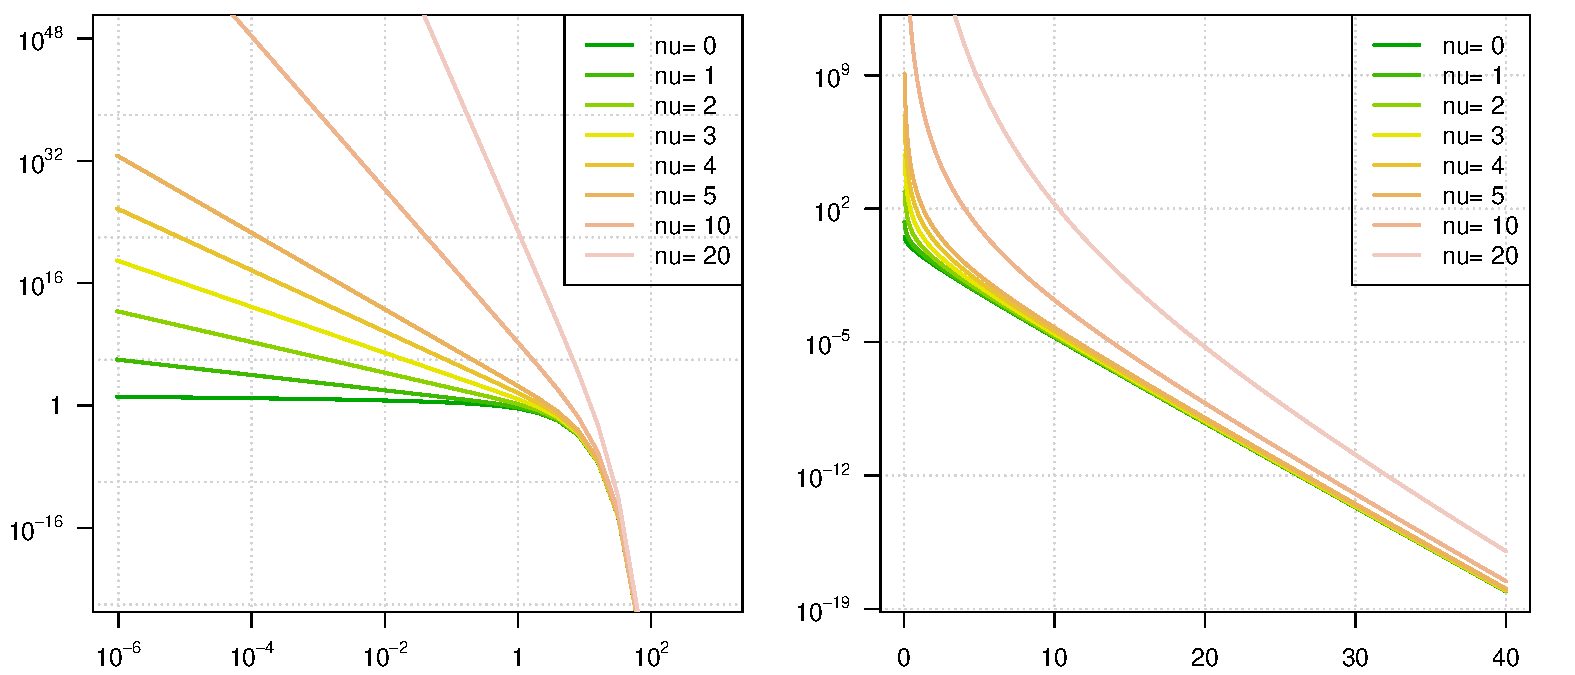
\includegraphics[width=0.7\linewidth]{figures/bessel} 

}

\caption{贝塞尔函数图像}\label{fig:Bessel-function}
\end{figure}

\hypertarget{Laplace-approximation}{%
\section{拉普拉斯近似}\label{Laplace-approximation}}

先回顾一下基本的泰勒展开,一个函数可以在点 \(a\)
处展开成和的形式,有时候是无穷多项,可以使用其中的有限项最为近似,通常会使用前三项,即到达二阶导的位置。

\[
f(x) = f(a) + \frac{f'(a)}{1!}(x-a) + \frac{f''(a)}{2!}(x-a)^2 + \frac{f'''(a)}{3!}(x-a)^3 + \ldots
\]

以基本的抛物线为例, \(f(x) = x^2\),在 \(a = 2\) 处展开

\[ f(x) = x^2, \quad f'(x) = 2x, \quad f''(x) = 2, \quad f'''(x) = 0 \]

因此,

\[ f(x) = x^2 = 2^2 + 2(2)(x-2) + \frac{2}{2}(x-2)^2 \]

拉普拉斯近似用正态分布来估计任意分布,它使用泰勒展开的前三项近似
\(\log g(x)\),展开的位置是 \(\hat{x}\),则

\[
\log g(x) \approx \log g(\hat{x}) + \frac{\partial \log g(\hat{x})}{\partial x} (x - \hat{x}) + \frac{\partial^2 \log g(\hat{x})}{2\partial x^2} (x - \hat{x})^2
\]

在函数 \(g(x)\) 的极值点 \(\hat{x}\) 展开, \(x = \hat{x}\) 一阶导是
0,用曲率去估计方差是
\(\hat{\sigma}^2 = -1/\frac{\partial^2 \log g(\hat{x})}{2\partial x^2}\),再重写上述近似

\[ \log g(x) \approx \log g(\hat{x}) - \frac{1}{2\hat{\sigma}^2} (x - \hat{x})^2 \]

现在,用这个结果做正态近似,将上式两端取指数和积分,移去常数项

\[
\int g(x) \mathrm{d}x = \int \exp[\log g(x)] \mathrm{d}x \approx \mathrm{constant} \int \exp[- \frac{(x - \hat{x})^2}{2\hat{\sigma}^2}] \mathrm{d}x
\]

拉普拉斯方法用正态分布近似分布 \(f(x)\), 其均值
\(\hat{x}\),可以通过求解 \(f'(x) = 0\) 获得,方差
\(\hat{\sigma}^2 = -1/f''(\hat{x})\)

以卡方分布 \(\chi^2\) 为例,

\begin{align*}
    f(x; k) & = \frac{ x^{k/2-1} \mathrm{e}^{-x/2} }{ 2^{k/2}\Gamma(k/2) }, x \geq 0 \\
  \log f(x) & = (k/2 - 1) \log x - x/2 \\
 \log f'(x) & = (k/2-1)/x - 1/2 = 0 \\
\log f''(x) & = -(k/2-1)/x^2
\end{align*}

所以

\[ \chi_{k}^2 \overset{LA}{\sim}  N(\hat{x} = k-2, \hat{\sigma}^2 = 2(k-2)) \]

自由度越大,近似效果越好,对于多元分布的情况不难推广,使用多元泰勒展开和黑塞矩阵即可表示。并且参数集
\(\theta\) 有唯一的极大值点 \(\hat{\theta}\) \citep{Tierney1986}

\hypertarget{Jeffreys-prior}{%
\section{Jeffreys 先验分布}\label{Jeffreys-prior}}

设 \(\mathbf{x} = (x_1,\ldots,x_n)\) 是来自密度函数 \(p(x|\theta)\)
的一个样本,其中 \(\boldsymbol{\theta} = (\theta_1,\ldots,\theta_p)\) 是
\(p\) 维参数向量。在对 \(\boldsymbol{\theta}\) 无任何先验信息可用时,
Jeffreys (1961年)利用变换群和 Harr 测度导出 \(\boldsymbol{\theta}\)
的无信息先验分布可用 Fisher
信息阵的行列式的平方根表示。这种无信息先验分布常称为 Jeffreys
先验分布。其求取步骤如下:

\begin{enumerate}
\def\labelenumi{\arabic{enumi}.}
\tightlist
\item
  写出样本的对数似然函数
  \(l(\boldsymbol{\theta}|x) = \sum_{i=1}^{n}\ln p(x_i | \theta)\);
\item
  算出参数 \(\boldsymbol{\theta}\) 的 Fisher 信息阵
  \[\mathbf{I}(\boldsymbol{\theta}) = \mathsf{E}_{x|\theta} \big( - \frac{\partial^2 l}{\partial \theta_i \partial \theta_j} \big)_{i,j=1,\ldots,p}\]
  在单参数场合,
  \(\mathbf{I}(\theta) = \mathsf{E}_{x|\theta} \big( - \frac{\partial^2 l}{\partial \theta^2} \big)\);
\item
  \(\boldsymbol{\theta}\) 的无信息先验密度函数为
  \(\pi(\boldsymbol{\theta}) = [\det \mathbf{I}(\theta) ]^{1/2}\),在单参数场合,
  \(\pi(\theta) = [\mathbf{I}(\theta) ]^{1/2}\)
\end{enumerate}

\hypertarget{bayes-methods}{%
\section{贝叶斯定理与先验分布}\label{bayes-methods}}

{非信息先验分布,扁平先验 flat prior,模糊先验}

以标准线性模型为例介绍贝叶斯分析及其基本概念
\citep{Rasmussen2006},为什么不用 RMSE 均方误差,WAIC pDIC 模型选择 loo
K-CV

贝叶斯定理 \ref{fig:bayes-theorem} 贝叶斯定理 \eqref{eq:bayes-theorem}

\begin{figure}

{\centering 
\includegraphics[width=0.7\linewidth]{figures/bayes-theorem} 

}

\caption{贝叶斯定理}\label{fig:bayes-theorem}
\end{figure}

作为铺垫,先结合 SGLMM
模型介绍一下贝叶斯定理,其中,\(\boldsymbol{\theta}\) 代表 SGLMM
模型中的参数,\(\mathbf{Y}\) 是响应变量对应的观察值。

\begin{align}
\begin{array}{rcll}
p(\boldsymbol{\theta}|\mathbf{Y})  & =  & \displaystyle \frac{p(\boldsymbol{\theta},\mathbf{Y})}{p(\mathbf{Y})}
& \mbox{ [条件概率定义]}
\\[16pt]
& = & \displaystyle \frac{p(\mathbf{Y}|\boldsymbol{\theta}) p(\boldsymbol{\theta})}{p(\mathbf{Y})}
& \mbox{ [链式法则]}
\\[16pt]
& = & \displaystyle \frac{p(\mathbf{Y}|\boldsymbol{\theta})p(\boldsymbol{\theta})}{\int_{\Theta}p(\mathbf{Y},\boldsymbol{\theta})d\boldsymbol{\theta}}
& \mbox{ [全概率公式]}
\\[16pt]
& = & \displaystyle \frac{p(\mathbf{Y}|\boldsymbol{\theta})p(\boldsymbol{\theta})}{\int_{\Theta}p(\mathbf{Y}|\boldsymbol{\theta})p(\boldsymbol{\theta})d\boldsymbol{\theta}}
& \mbox{ [链式法则]}
\\[16pt]
& \propto & \displaystyle p(\mathbf{Y}|\boldsymbol{\theta})p(\boldsymbol{\theta})
& \mbox{ [$\mathbf{Y}$ 已知]}
\end{array} \label{eq:bayes-theorem}
\end{align}

\hypertarget{Curse-of-Dimensionality}{%
\section{维数灾难与蒙特卡罗积分}\label{Curse-of-Dimensionality}}

一般地,混合效应模型的统计推断总是不可避免的要面对高维积分,处理高维积分的方法一个是寻找近似方法避免求积分,一个是寻找有效的随机模拟方法直接求积分。这里,介绍蒙特卡罗方法求积分,以计算
\(N\) 维超立方体的内切球的体积为例说明。

假设我们有一个 \(N\) 维超立方体,其中心在坐标
\(\mathbf{0} = (0,\ldots,0)\)。超立方体在点
\((\pm 1/2,\ldots,\pm 1/2)\),有 \(2^{N}\)
个角落,超立方体边长是1,\(1^{N}=1\),所以它的体积是1。

如果 \(N=1\),超立方体是一条从 \(-\frac{1}{2}\) 到 \(\frac{1}{2}\)
的单位长度的线,如果 \(N=2\),超立方体是一个单位正方形,对角是
\(\left( -\frac{1}{2}, -\frac{1}{2} \right)\) 和
\(\left( \frac{1}{2}, \frac{1}{2} \right)\),如果
\(N=3\),超立方体就是单位体积的立方体,对角是
\(\left( -\frac{1}{2}, -\frac{1}{2}, -\frac{1}{2} \right)\) 和
\(\left( \frac{1}{2}, \frac{1}{2}, \frac{1}{2} \right)\),依此类推,\(N\)
维超立方体体积是1,对角是
\(\left( -\frac{1}{2}, \ldots, -\frac{1}{2} \right)\) 和
\(\left( \frac{1}{2}, \ldots, \frac{1}{2} \right)\)

现在,考虑 \(N\) 维超立方体的内切球,我们把它称为 \(N\)
维超球,它的中心在原点,半径是 \(\frac{1}{2}\)。我们说点 \(y\)
在超球内,意味着它到原点的距离小于半径,即 \(\| y \| < \frac{1}{2}\)。

一维情形下,超球是从的线,包含了整个超立方体。二维情形下,超球是中心在原点,半径为
\(\frac{1}{2}\) 的圆。三维情形下,超球是立方体的内切球。

我们知道单位超立方体的体积是1,但是其内的内切球的体积是多少呢?我们已经学过如何去定义一个积分计算半径为
\(r\) 的二维球(即圆)的体积(即面积)是
\(\pi r^2\),三维情形下,内切球是
\(\frac{4}{3}\pi r^3\)。但是更高维的欧式空间里,内切球的体积是多少呢?

我们当然可以去计算越来越复杂的多重积分,但是这里我们介绍采样的方法去计算积分,即所谓的蒙特卡罗方法,由乌拉姆
(S. Ulam)、冯\(\cdot\)诺依曼(J. von Neumann) 和梅特罗波利斯 (N.
Metropolis) 等
在美国核武器研究实验室创立,当时正值二战期间,为了研制原子弹,出于保密的需要,与随机模拟相关的技术就代号蒙特卡罗。现在,蒙特卡罗方法占据现代统计计算的核心地位,特别是与贝叶斯相关的领域。

用蒙特卡罗方法去计算单位超立方体内的超球,首先我们需要在单位超立方体内产生随机点,然后计算落在超球内点的比例,即超球的体积。随着点的数目增加,估计的体积会收敛到真实的体积。因为这些点都独立同均匀分布,根据中心极限定理,误差下降的比率是
\(\mathcal{O}\left( 1 / \sqrt{n} \right)\),这也意味着每增加一个小数点的准确度,样本量要增加
100 倍。

表 \ref{tab:calculate-volume-of-hyperball}
列出了前10维超球的体积,随着维数的增加,超球的体积迅速变小,超立方体内随机点的个数是
100000。这里有一个反直观的现象,内切球的体积竟然随着维数的增加变小,并且在10维的情形下,内切球的体积已不到超立方体的
0.3\%。

\begin{longtable}[]{@{}lcccccccccc@{}}
\caption{\label{tab:calculate-volume-of-hyperball}
前10维单位超立方体内切球的体积(已经四舍五入保留小数点后三位)}\tabularnewline
\toprule
维数 & 1 & 2 & 3 & 4 & 5 & 6 & 7 & 8 & 9 & 10\tabularnewline
\midrule
\endfirsthead
\toprule
维数 & 1 & 2 & 3 & 4 & 5 & 6 & 7 & 8 & 9 & 10\tabularnewline
\midrule
\endhead
体积 & 1.000 & 0.784 & 0.525 & 0.307 & 0.166 & 0.081 & 0.037 & 0.016 &
0.006 & 0.0027\tabularnewline
\bottomrule
\end{longtable}

\hypertarget{Samplers}{%
\section{采样器与 Stan}\label{Samplers}}

随机模拟的基础是有高质量的伪随机数,如何生成和检验伪随机数的质量参见黄湘云的文章
\citep{Huang2017COS}。通过随机模拟的方式从总体中获取样本,需要一个抽样(也叫采样)的过程,不同的采样算法(也叫采样器)在适用范围和采样效率方面有不同。在贝叶斯计算中,常用的采样器有
Gibbs, Metropolis 和汉密尔顿蒙特卡罗 (Hamiltonian Monte Carlo,简称
HMC) 三类。

Matthew D. Hoffman 和 Andrew Gelman (2014年) \citep{hoffman2014} 提出的
No-U-Turn 采样器属于 HMC 方法 衍生的采样器。

Stan 是一门基于 C++
的高级编程语言,用户只需提供数据、模型和参数初值,目标后验分布的 Markov
链的模拟过程是自动实现的。除了可以完全在 Stan 脚本中写模型外,Stan
还提供其他编程语言的接口,如 R,Python 和 MATLAB
等,使得熟悉其他编程语言的用户也可以比较方便地调用。与 Python、R
这类解释型编程语言不同, Stan 代码需要先翻译成 C++ 代码,然后编译执行。

Donald B. Rubin (1981年) \citep{Rubin1981} 分析了 Donald L. Alderman 和
Donald E. Powers \citep{Alderman1980} 收集的原始数据,得出表
\ref{tab:eight-high-schools}, Andrew Gelman 和 John B. Carlin 等
(2003年) \citep{Gelman2003} 建立分层正态模型
\eqref{eq:hierarchical-normal-models} 分析 Eight Schools
数据集,这里再次以该数据集和模型为例介绍 Stan 的使用和算法实现。

\begin{equation}
\begin{aligned}
     \mu & \sim \mathcal{N}(0,5) \\
    \tau & \sim \text{Half-Cauchy}(0,5) \\
p(\mu,\tau) & \propto 1 \\
  \eta_i & \sim \mathcal{N}(0,1) \\
\theta_i &  =   \mu + \tau \cdot \eta_i \\
     y_i & \sim \mathcal{N}(\theta_i,\sigma^2_{i})
\end{aligned}
\label{eq:hierarchical-normal-models}
\end{equation}

由美国教育考试服务调查搜集,用以分析不同的辅导项目对学生考试分数的影响,调查结果用来帮助高校招生。分别随机调查了
8 所高中,输出变量是一个分数,培训效应的估计 \(y_j\),其样本方差
\(\sigma^2_j\),数据集见表 \ref{tab:eight-high-schools}。

\begin{longtable}[]{@{}ccccccccc@{}}
\caption{\label{tab:eight-high-schools} Eight Schools 数据集}\tabularnewline
\toprule
School & A & B & C & D & E & F & G & H\tabularnewline
\midrule
\endfirsthead
\toprule
School & A & B & C & D & E & F & G & H\tabularnewline
\midrule
\endhead
\(y_i\) & 28 & 8 & -3 & 7 & -1 & 1 & 18 & 12\tabularnewline
\(\sigma_i\) & 15 & 10 & 16 & 11 & 9 & 11 & 10 & 18\tabularnewline
\bottomrule
\end{longtable}

分层正态模型可以在 Stan 中写成如下形式,在工作目录下把它保存为
\texttt{8schools.stan}

\begin{verbatim}
// saved as 8schools.stan
data {
  int<lower=0> J; // number of schools 
  real y[J]; // estimated treatment effects
  real<lower=0> sigma[J]; // s.e. of effect estimates 
}
parameters {
  real mu; // population mean
  real<lower=0> tau; // population sd
  real eta[J]; // school-level errors
}
transformed parameters {
  real theta[J];  // schools effects
  for (j in 1:J)
    theta[j] = mu + tau * eta[j];
  // theta = mu + tau*eta;
}
model {
  // set prior for mu or uniform prior distribution default
  // target += normal_lpdf(mu  | 0, 10); 
  // target += cauchy_lpdf(tau | 0, 25); # the same as mu
  target += normal_lpdf(eta | 0, 1);
  target += normal_lpdf(y | theta, sigma); // target distribution
  // y ~ normal(theta, sigma);
}
\end{verbatim}

上述 Stan 代码的第一段提供数据:学校的数目 \(J\),估计值
\(y_1,\ldots,y_{J}\),标准差
\(\sigma_1,\ldots,\sigma_{J}\),数据类型可以是整数、实数,结构可以是向量,或更一般的数组,还可以带约束,如在这个模型中
\(J\) 限制为非负, \(\sigma_{J}\) 必须是正的,另外两个反斜杠 //
表示注释。

第二段代码声明参数:模型中的待估参数,学校总体的效应 \(\theta_j\),均值
\(\mu\),标准差 \(\tau\),学校水平上的误差 \(\eta\) 和效应
\(\theta\)。在这个模型中,用 \(\mu,\tau,\eta\) 表示 \(\theta\)
而不是直接声明 \(\theta\)
作一个参数,通过这种参数化,采样器的运行效率会提高,还应该尽量使用向量化操作代替
for 循环语句。

最后一段是模型:稍微注意的是,正文中正态分布 \(N(\cdot,\cdot)\)
中后一个位置是方差,而 Stan
代码中使用的是标准差。\texttt{target\ +=\ normal\_lpdf(y\ \textbar{}\ theta,\ sigma)}
和 \texttt{y\ \textasciitilde{}\ normal(theta,\ sigma)}
对模型的贡献是一样的,都使用正态分布的对数概率密度函数,只是后者扔掉了对数密度函数的常数项而已,这对于
Stan 的采样、近似或优化算法没有影响 \citep{Stan2017JSS}。

算法运行的硬件环境是 16 核 32 线程主频 2.8 GHz 英特尔至强 E5-2680
处理器,系统环境 CentOS 7,R 软件版本 3.5.1,RStan 版本 2.17.3。

HMC算法参数主要设置了4条链,每条链迭代 10000
次,为复现模型结果随机数种子设为 2018

\begin{longtable}[]{@{}lrrrrrrrrrr@{}}
\caption{\label{tab:eight-schools-output} 对 Eight Schools
数据集建立分层正态模型 \eqref{eq:hierarchical-normal-models},采用 HMC
算法估计模型参数值}\tabularnewline
\toprule
& mean & se\_mean & sd & 2.5\% & 25\% & 50\% & 75\% & 97.5\% & n\_eff &
Rhat\tabularnewline
\midrule
\endfirsthead
\toprule
& mean & se\_mean & sd & 2.5\% & 25\% & 50\% & 75\% & 97.5\% & n\_eff &
Rhat\tabularnewline
\midrule
\endhead
\(\mu\) & 7.99 & 0.05 & 5.02 & -1.65 & 4.75 & 7.92 & 11.15 & 18.10 &
8455 & 1\tabularnewline
\(\tau\) & 6.47 & 0.06 & 5.44 & 0.22 & 2.45 & 5.18 & 9.07 & 20.50 & 7375
& 1\tabularnewline
\(\eta_1\) & 0.40 & 0.01 & 0.93 & -1.49 & -0.21 & 0.42 & 1.02 & 2.19 &
16637 & 1\tabularnewline
\(\eta_2\) & 0.00 & 0.01 & 0.87 & -1.73 & -0.58 & 0.00 & 0.57 & 1.70 &
16486 & 1\tabularnewline
\(\eta_3\) & -0.20 & 0.01 & 0.93 & -1.99 & -0.82 & -0.20 & 0.41 & 1.66 &
20000 & 1\tabularnewline
\(\eta_4\) & -0.04 & 0.01 & 0.88 & -1.80 & -0.60 & -0.04 & 0.53 & 1.74 &
20000 & 1\tabularnewline
\(\eta_5\) & -0.36 & 0.01 & 0.88 & -2.06 & -0.94 & -0.38 & 0.20 & 1.42 &
15489 & 1\tabularnewline
\(\eta_6\) & -0.22 & 0.01 & 0.90 & -1.96 & -0.82 & -0.23 & 0.37 & 1.57 &
20000 & 1\tabularnewline
\(\eta_7\) & 0.34 & 0.01 & 0.89 & -1.49 & -0.24 & 0.36 & 0.93 & 2.04 &
16262 & 1\tabularnewline
\(\eta_8\) & 0.05 & 0.01 & 0.94 & -1.81 & -0.57 & 0.06 & 0.69 & 1.91 &
20000 & 1\tabularnewline
\(\theta_1\) & 11.45 & 0.08 & 8.27 & -1.86 & 6.07 & 10.27 & 15.50 &
31.68 & 11788 & 1\tabularnewline
\(\theta_2\) & 7.93 & 0.04 & 6.15 & -4.45 & 3.99 & 7.90 & 11.74 & 20.44
& 20000 & 1\tabularnewline
\(\theta_3\) & 6.17 & 0.06 & 7.67 & -11.17 & 2.07 & 6.74 & 10.89 & 19.94
& 16041 & 1\tabularnewline
\(\theta_4\) & 7.66 & 0.05 & 6.51 & -5.63 & 3.75 & 7.72 & 11.62 & 20.78
& 20000 & 1\tabularnewline
\(\theta_5\) & 5.13 & 0.05 & 6.41 & -9.51 & 1.37 & 5.66 & 9.43 & 16.41 &
20000 & 1\tabularnewline
\(\theta_6\) & 6.14 & 0.05 & 6.66 & -8.63 & 2.35 & 6.58 & 10.40 & 18.47
& 20000 & 1\tabularnewline
\(\theta_7\) & 10.64 & 0.05 & 6.76 & -1.14 & 6.11 & 10.11 & 14.52 &
25.88 & 20000 & 1\tabularnewline
\(\theta_8\) & 8.42 & 0.06 & 7.86 & -7.24 & 3.91 & 8.26 & 12.60 & 25.24
& 16598 & 1\tabularnewline
lp\_\_ & -39.55 & 0.03 & 2.64 & -45.41 & -41.15 & -39.31 & -37.67 &
-35.12 & 6325 & 1\tabularnewline
\bottomrule
\end{longtable}

表 \ref{tab:eight-schools-output} 的列为后验量的估计值:依次是均值
\(\mathsf{E}(\mu|Y)\)、 标准误(standard error)
\(\mathsf{Var}(\mu|Y)\)、标准差 (standard deviation)
\(\mathsf{E}(\sigma|Y)\) 、后验分布的 5 个分位点、有效样本数 \(n_{eff}\)
和潜在尺度缩减因子 (potential scale reduction factor),最后两个量
用来分析采样效率;最后一行表示每次迭代的未正则的对数后验密度
(unnormalized log-posterior density)
\(\hat{R}\),当链条都收敛到同一平稳分布的时候,\(\hat{R}\) 接近 1。

这里我们对 \(\tau\) 采用的非信息先验分布是均匀先验,参数 \(\tau\) 的
95\% 的置信区间是 (0.22,20.5), 数据支持 \(\tau\) 的范围低于

\begin{figure}

{\centering 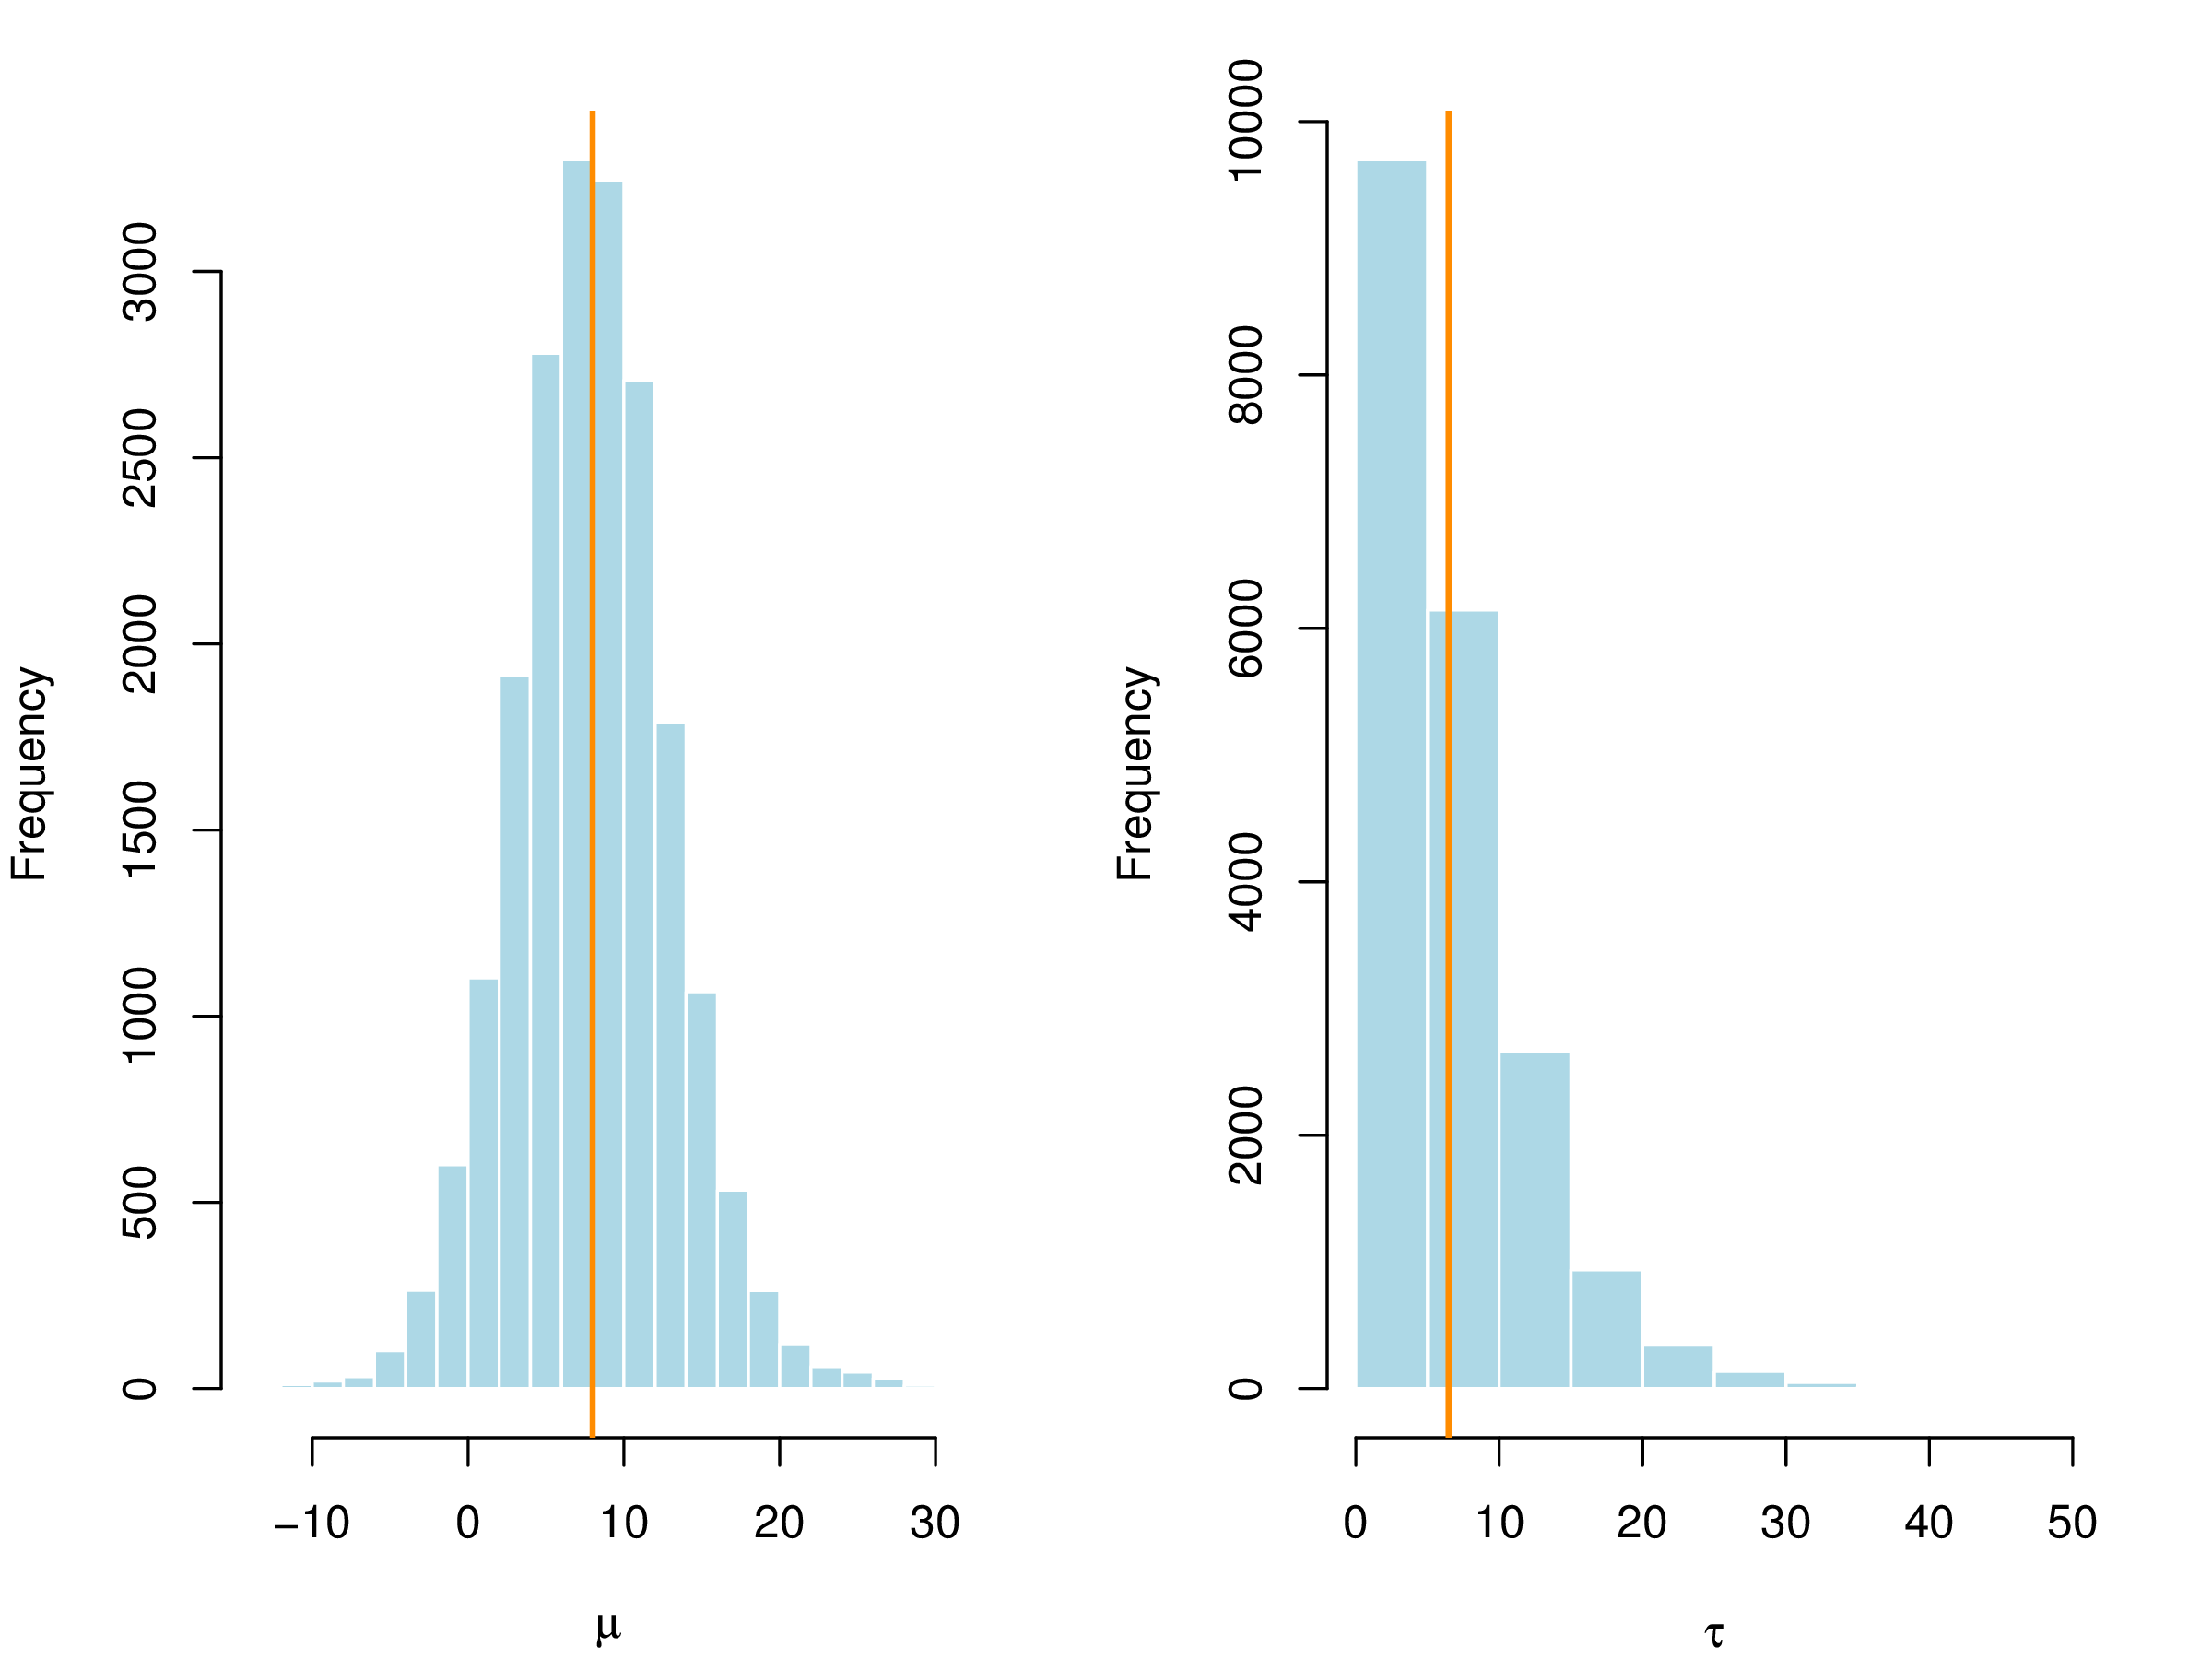
\includegraphics[width=0.7\linewidth]{figures/posterior_mu_tau} 

}

\caption{对 $\mu,\tau$ 给定均匀先验,后验均值 $\mu$ 和标准差 $\tau$ 的直方图}\label{fig:posterior-mu-tau}
\end{figure}

为了得到可靠的后验估计,做出合理的推断,诊断序列的平稳性是必不可少的部分

\begin{figure}

{\centering \subfloat[诊断序列的平稳性\label{fig:diagnostic1}]{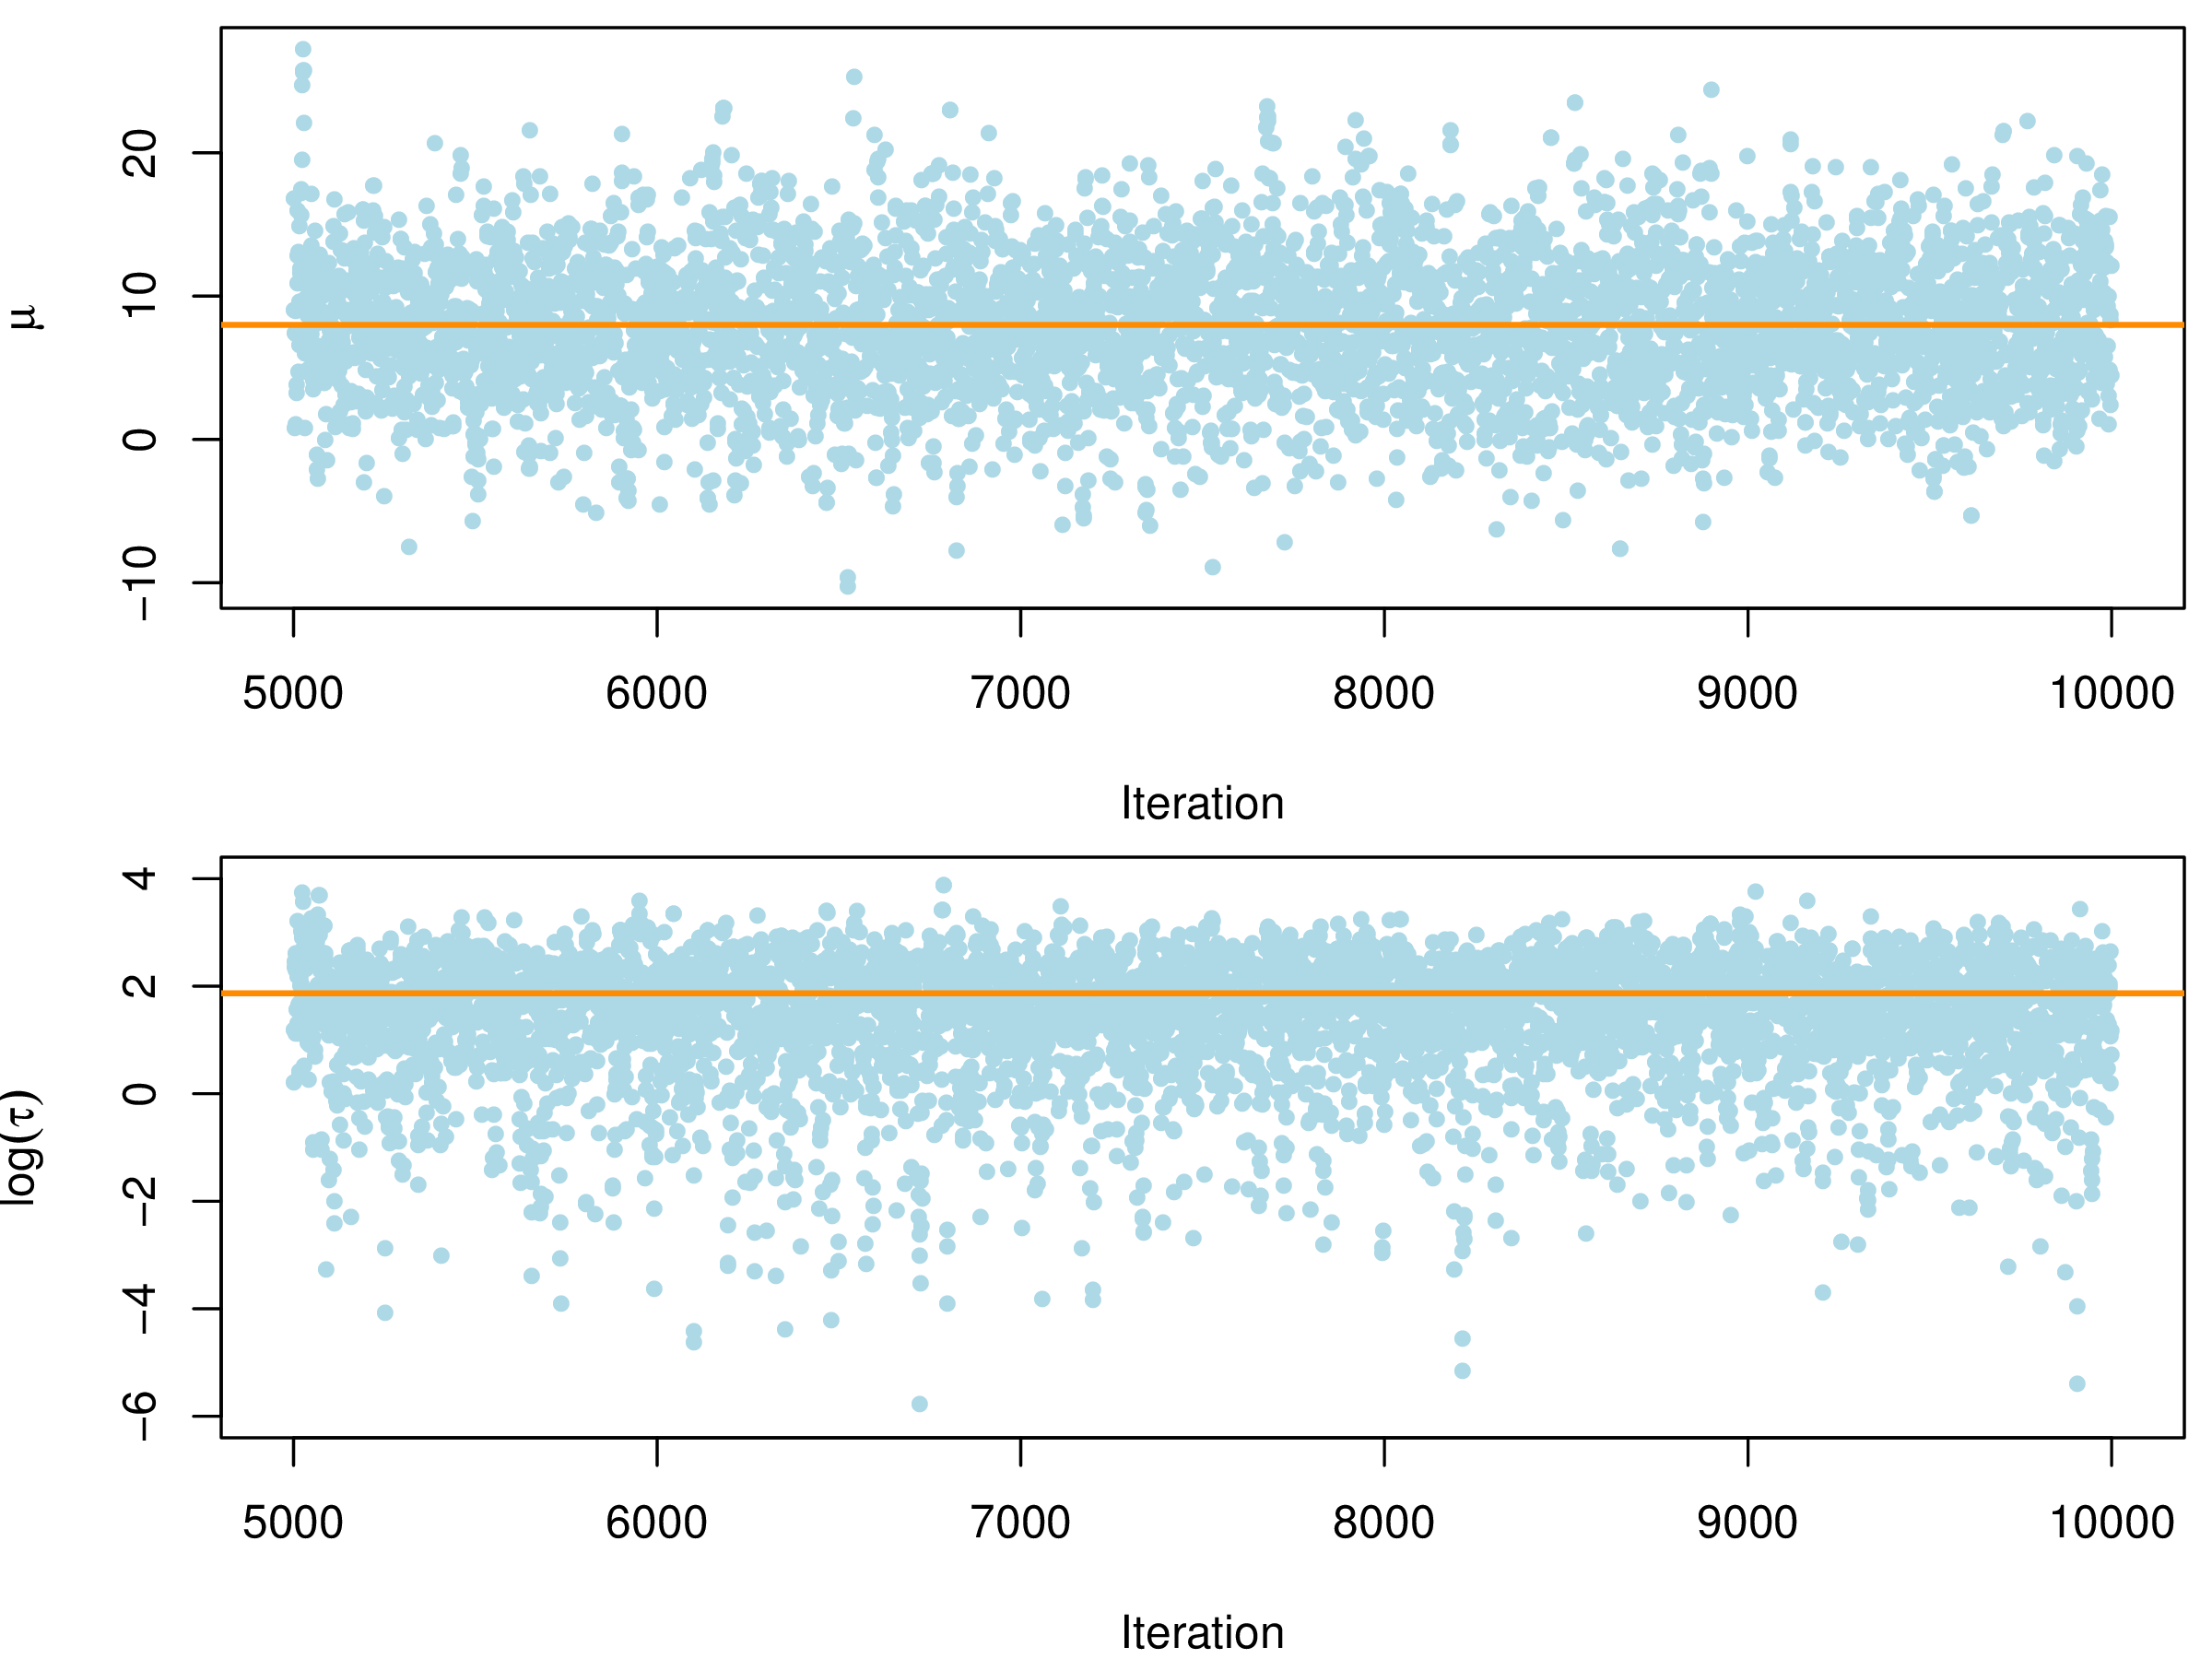
\includegraphics[width=0.7\linewidth]{figures/trace_mu_log_tau} }\\\subfloat[蒙特卡罗均值误差和发散点\label{fig:diagnostic2}]{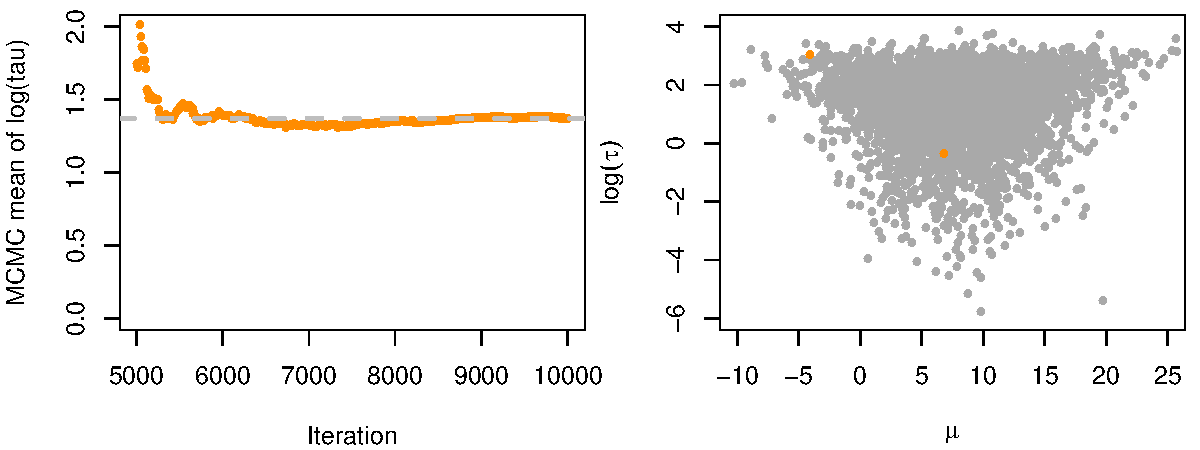
\includegraphics[width=0.7\linewidth]{figures/mcmc_mean_tau_div} }

}

\caption{诊断图}\label{fig:diagnostic}
\end{figure}

\section{方差缩减因子}

为了评估链条之间和内部的混合效果,我们引入潜在尺度缩减因子
\(\hat{R}\),对每个待估的量 \(\omega\),模拟产生 \(m\) 条链,每条链有
\(n\) 次迭代值 \(\omega_{ij} (i = 1,\ldots,n;j=1,\ldots,m)\),用 \(B\)
和 \(W\) 分别表示链条之间(不妨看作组间方差)和内部的方差(组内方差)

\begin{equation}
\begin{aligned}
& B = \frac{n}{m-1}\sum_{j=1}^{m}(\bar{\omega}_{.j} - \bar{\omega}_{..} ), \quad \bar{\omega}_{.j} = \frac{1}{n}\sum_{i=1}^{n}\omega_{ij}, \quad \bar{\omega}_{..} = \frac{1}{m}\sum_{j=1}^{m} \bar{\omega}_{.j}\\
& W = \frac{1}{m}\sum_{j=1}^{m}s^{2}_{j}, \quad s^{2}_{j} = \frac{1}{n-1}\sum_{i=1}^{n}(\omega_{ij} - \bar{\omega}_{.j})^2
\end{aligned} \label{eq:potential-scale-reduction}
\end{equation}

\(\omega\) 的边际后验方差 \(\mathsf{\omega|Y}\) 是 \(W\) 和 \(B\)
的加权平均

\begin{equation}
\widehat{\mathsf{Var}}^{+}(\omega|Y) = \frac{n-1}{n} W + \frac{1}{n} B 
\end{equation}

当初始分布发散 (overdispersed)
时,这个量会高估边际后验方差,但在链条平稳或 \(n \to \infty\)
时,它是无偏的。同时,对任意有限的 \(n\),组内方差 \(W\) 应该会低估
\(\mathsf{Var}(\omega|Y)\),因为单个链条没有时间覆盖目标分布;在
\(n \to \infty\), \(W\) 的期望会是 \(\mathsf{Var}(\omega|Y)\)。

我们通过估计潜在尺度缩减因子 \(\hat{R}\) 检测链条的收敛性

\begin{equation}
\hat{R} = \sqrt{\frac{\widehat{\mathsf{Var}}^{+}(\omega|Y)}{W}}
\end{equation}

随着 \(n \to \infty\), \(\hat{R}\) 下降到 1。如果 \(\hat{R}\)
比较大,我们有理由认为需要增加模拟次数以改进待估参数 \(\omega\)
的后验分布 \citep{Gelman2013R}。

\hypertarget{models}{%
\chapter{统计模型}\label{models}}

第 \ref{Linear-Models} 节,第 \ref{Generalized-Linear-Models} 节和第
\ref{Generalized-Linear-Mixed-Effects-Models} 节简略介绍了线性模型,
广义线性模型和广义线性混合效应模型及其数学表示,
并随同模型给出了模型求解的 R 包或函数,
为空间广义线性混合效应模型的介绍做铺垫。第
\ref{Spatial-Generalized-linear-mixed-effects-models}
节重点介绍了空间广义线性混合效应模型(以下简称为 SGLMM 模型),
并分三小节介绍模型中的重要成分, 第 小节介绍 SGLMM 模型中的空间效应,
即平稳空间高斯过程, 第 \ref{covariance-function}
小节介绍影响空间效应结构的关键部分 ---
自协方差函数和平稳空间高斯过程的核函数或自相关函数, 第 \ref{identify}
小节介绍非空间的随机效应,在地质统计中常称为块金效应,以及它带来的 SGLMM
模型可识别问题与相应处理方式。

\hypertarget{Linear-Models}{%
\section{线性模型}\label{Linear-Models}}

线性模型的一般形式为

\begin{equation}
Y = X^{\top}\beta + \epsilon, \mathrm{E}(\epsilon) = 0, \mathrm{Cov}(\epsilon) = \sigma^2\mathbf{I}  \label{eq:LM}
\end{equation}

\noindent 其中,\(Y = (y_1,y_2,\ldots,y_n)^{\top}\) 是 \(n\)
维列向量,代表对响应变量 \(Y\) 的 \(n\) 次观测;
\(\beta = (\beta_0,\beta_1,\ldots,\beta_{p-1})^{\top}\) 是 \(p\)
维列向量, 代表模型 \eqref{eq:LM} 的协变量 \(X\) 的系数,\(\beta_0\)
是截距项;
\(X^{\top} = (1_{(1\times n)}^{\top},X_{(1)}^{\top},X_{(2)}^{\top},\ldots,X_{(p-1)}^{\top})\),
\(1_{(1\times n)}^{\top}\) 是全 1 的 \(n\) 维列向量,而
\(X_{(i)}^{\top} = (x_{1i},x_{2i},\ldots,x_{ni})^{\top}\) 代表对第 \(i\)
个自变量的 \(n\) 次观测;
\(\epsilon = (\epsilon_1,\epsilon_2,\ldots,\epsilon_n)^{\top}\) 是 \(n\)
维列向量,代表模型的随机误差,并且假定
\(\mathrm{E}(\epsilon_i \epsilon_j) = 0, i \ne j\),
即模型误差项之间线性无关,且方差齐性,都是 \(\sigma^2(>0)\)。 估计模型
\eqref{eq:LM} 的参数常用最小二乘和最大似然方法, 求解线性模型 \eqref{eq:LM}
的参数可以用 R 函数
\texttt{lm},近年来,高维乃至超高维稀疏线性模型成为热门的研究方向,相关的
R 包也越来越多,比较流行的有 \textbf{glmnet} \citep{glmnet2011JSS} 和
\textbf{SIS} \citep{SIS2016JSS}。

\hypertarget{Generalized-Linear-Models}{%
\section{广义线性模型}\label{Generalized-Linear-Models}}

广义线性模型的一般形式

\begin{equation}
g(\mu) = X^{\top}\beta  \label{eq:GLM}
\end{equation}

\noindent 其中,\(\mu \equiv \mathrm{E}(Y)\), \(g\)
代表联系函数,特别地,当 \(Y \sim N(\mu,\sigma^2)\) 时,联系函数
\(g(x) = x\),模型 \eqref{eq:GLM} 变为一般线性模型 \eqref{eq:LM}。当
\(Y \sim \mathrm{Binomial}(n,p)\) 时,响应变量 \(Y\) 的期望
\(\mu =\mathrm{E}(Y) = np\), 联系函数 \(g(x)=\ln(\frac{x}{1-x})\),模型
\eqref{eq:GLM} 变为\(\log(\frac{p}{1-p})=X^{\top}\beta\)。 当
\(Y \sim \mathrm{Possion}(\lambda)\) 时,响应变量 \(Y\) 的期望
\(\mu =\mathrm{E}(Y) = \lambda\), 联系函数\(g(x) = \ln(x)\), 模型
\eqref{eq:GLM} 变为 \(\log(\lambda) = X^{\top}\beta\)。
指数族下其余分布对应的联系函数此处不一一列举, 完整列表可以参看 1989 年
McCullagh 和 Nelder 所著的《广义线性模型》 \citep{McCullagh1989}。 模型
\eqref{eq:GLM} 最早由 Nelder 和 Wedderburn
在1972年提出\citep{Nelder1972},它弥补了模型 \eqref{eq:LM}
的两个重要缺点: 一是因变量只能取连续值的情况,
二是期望与自变量只能用线性关系联系 \citep{Chen2011}。 求解广义线性模型
\eqref{eq:GLM} 的 R 函数是 \texttt{glm}, 常用拟似然法去估计模型
\eqref{eq:GLM} 的参数。

\hypertarget{Generalized-Linear-Mixed-Effects-Models}{%
\section{广义线性混合效应模型}\label{Generalized-Linear-Mixed-Effects-Models}}

广义线性混合模型的一般形式

\begin{equation}
g(\mu) = X^{\top}\boldsymbol{\beta} + Z^{\top}\mathbf{b}  \label{eq:GLMM}
\end{equation}

\noindent 其中, \(Z^{\top}\) 是 \(q\) 维随机效应 \(\mathbf{b}\) 的
\(n \times q\)
的数据矩阵,其它符号含义如前所述。广义线性混合效应模型中既包含固定效应
\(\boldsymbol{\beta}\) 又包含随机效应 \(\mathbf{b}\) 。 线性模型
\eqref{eq:LM} 和广义线性模型 \eqref{eq:GLM} 中的协变量都是固定效应,
而随机效应是那些不能直接观察到的潜效应, 但是对响应变量却产生显著影响。
特别是在基因变异位点与表现型的关系研究中,
除了用最新科技做全基因组扫描获取显著的基因位点,
还应该把那些看似不显著, 联合在一起却显著的位点作为随机效应去考虑
\citep{Yang2010Common}。求解模型 \eqref{eq:GLMM}的 R 包有 \textbf{nlme}
,\textbf{mgcv} 和 \textbf{lme4}, 参数估计的方法一般有限制极大似然法。
除了求解模型 \eqref{eq:GLMM} 外, \textbf{nlme}
可以拟合一些非线性混合效应模型, \textbf{mgcv}
可以拟合广义可加混合效应模型, \textbf{lme4} 使用了高性能的 Eigen
数值代数库,可以加快模型的求解过程。

\hypertarget{Spatial-Generalized-linear-mixed-effects-models}{%
\section{空间广义线性混合效应模型}\label{Spatial-Generalized-linear-mixed-effects-models}}

在提出 SGLMM
模型之前,先介绍空间高斯过程,然后是平稳空间高斯过程和SGLMM模型结构,以步步推进的方式引入各成分的假设条件,其后着重阐述了空间效应的自相关函数,它决定空间效应,包含模型中的待估参数。

\hypertarget{intro-sglmm}{%
\subsection{模型结构}\label{intro-sglmm}}

空间广义线性混合效应模型是对模型 \eqref{eq:GLMM}
的进一步延伸,其一般形式为

\begin{equation}
g(\mu_i) = d(x_i)^{\top}\beta + S(x_i) + Z_i \label{eq:SGLMM}
\end{equation}

\noindent 其中,\(d^{\top}(x_i)\) 表示协变量对应的观测数据向量,即 \(p\)
个协变量在第 \(i\) 个位置 \(x_i\) 的观察值。 此外, 假定
\(\mathcal{S} = \{S(x): x \in \mathbb{R}^2\}\) 是均值为0, 方差为
\(\sigma^2\),平稳且各向同性的空间高斯过程,
\(\rho(x,x') = \mathrm{Corr}\{S(x),S(x')\} \equiv \rho(\|x,x'\|)\),
\(\|\cdot\|\) 表示距离, 样本之间的位置间隔不大就用欧氏距离,
间隔很大可以考虑用球面距离; \(S(x_i)\) 代表了与空间位置 \(x_i\)
相关的随机效应, 简称空间效应; 这里,
\(Z_i \stackrel{i.i.d}{\sim} N(0,\tau^2)\) 的非空间随机效应,
也称块金效应 (nugget effect), 一般解释为测量误差 (measurement error)
或微观变化 (micro-scale variation) \citep{Christensen2004}, 即
\(\tau^2=\mathrm{Var}(Y_{i}|S(x_{i})),\forall i = 1,2, \ldots, N\),
\(N\) 是采样点的数目, 其它符号含义不变。

\hypertarget{covariance-function}{%
\subsection{协方差函数}\label{covariance-function}}

随机过程的协方差函数,也称核函数,如无特殊说明,文中所指都是自协方差函数,模型
\eqref{eq:SGLMM} 的空间效应结构由相关函数决定, 在给出相关函数之前,
先计算一下空间效应的理论变差 \(V(x,x')\),
即空间过程的协方差函数的一半, 变差源于采矿术语, 和线性预测 \(T_{i}\)
的变差 \(V_{T}(u_{ij})\)。 为方便起见,记
\(T_{i} = d(x_i)^{\top}\beta + S(x_i) + Z_i\)

\begin{equation}
\begin{aligned}
V(x,x') 
&= \frac{1}{2}\mathrm{Var}\{S(x)-S(x')\}\\
&= \frac{1}{2}\mathrm{Cov}(S(x)-S(x'),S(x)-S(x'))\\
&= \frac{1}{2}\{E[S(x)-S(x')][S(x)-S(x')]-[E(S(x)-S(x'))]^2\}\\
&= \sigma^2-\mathrm{Cov}(S(x),S(x'))=\sigma^2\{1-\rho(u)\}\\
V_{T}(u_{ij})
&= \frac{1}{2}\mathrm{Var}\{T_{i}(x)-T_{j}(x)\} \\
&= \frac{1}{2}\mathrm{E}[(T_{i}-T_{j})^2]=\tau^2+\sigma^2(1-\rho(u_{ij})) 
\end{aligned} \label{eq:variograms}
\end{equation}

\noindent 从方程 \eqref{eq:variograms} 不难看出系数 \(\frac{1}{2}\)
的化简作用,类似地,根据协方差定义可推知随机向量
\(T = (T_1,T_2,\ldots,T_n)\) 的协方差矩阵如下:

\begin{equation}
\begin{aligned}
\mathrm{Cov}(T_{i}(x),T_{i}(x)) &= \mathrm{E}[S(x_i)]^2 + \mathrm{E}Z_{i}^{2}= \sigma^2+\tau^2 \\
\mathrm{Cov}(T_{i}(x),T_{j}(x)) &= \mathrm{E}[S(x_i)S(x_j)]  = \sigma^2\rho(u_{ij})
\end{aligned}
\end{equation}

\noindent 相关函数 \(\rho(u)\)
的作用和地位就显而易见了,它是既决定理论变差又决定协方差矩阵的结构。

\begin{figure}

{\centering 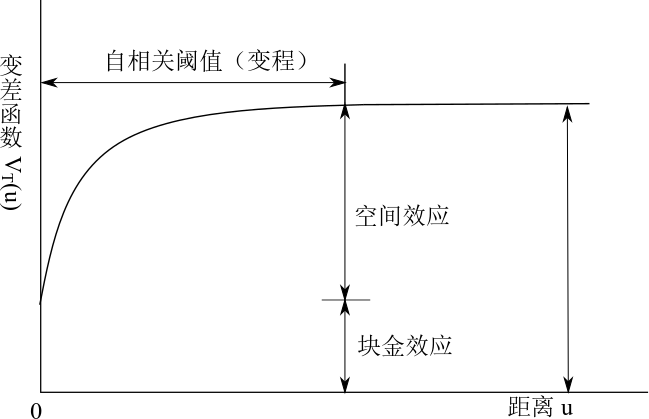
\includegraphics[width=0.7\linewidth]{figures/semi-variance} 

}

\caption{变差函数 $V_{T}(u)$ 示意图}\label{fig:semi-variance}
\end{figure}

常见的自相关函数族有高斯协方差函数、球面协方差函数和 Matérn 协方差函数:

\begin{equation}
\rho(u)=\{2^{\kappa -1}\Gamma(\kappa)\}^{-1}(u/\phi)^{\kappa}\mathcal{K}_{\kappa}(u/\phi),u > 0 \label{eq:matern1}
\end{equation}

\noindent 一般地,假定 \(\rho(u)\)
单调不增,即任何两样本之间的相关性应该随距离变大而减弱,尺度参数
\(\phi\) 控制函数 \(\rho(u)\) 递减到0的速率。方便起见,记
\(\rho(u) = \rho_{0}(u/\phi)\),则方程 \eqref{eq:matern1} 可简记为

\begin{equation}
\rho_{0}(u)=\{2^{\kappa -1}\Gamma(\kappa)\}^{-1}(u)^{\kappa}\mathcal{K}_{\kappa}(u),u > 0 \label{eq:matern2}
\end{equation}

\noindent 其中,\(\mathcal{K}_{\kappa}(\cdot)\) 是阶数为 \(\kappa\)
的第二类修正的贝塞尔函数, \(\kappa(>0)\)
是平滑参数,满足这些条件的空间过程 \(\mathcal{S}\) 是
\(\lceil\kappa\rceil-1\) 次均方可微的。

值得注意的是 Matérn 族其实包含幂指数族 \noindent 当
\(\kappa = 0.5\)时,\(\rho_{0}(u) = \exp(-u)\), \(S(x)\)
均方连续但是不可微,当 \(\kappa \to \infty\) 时,
\(\rho_{0}(u) = \exp(-u^2)\), \(S(x)\) 无限次均方可微。

实际操作中,估计 \(\kappa\),
为了节省计算,又不失一般性,经验做法是取离散的 \(\kappa\) 先验,如
\(\kappa = 0.5, 1.5, 2.5\), 分别对应 \(S(x)\)
均方连续、一次可微和二次可微。实际上,\(\rho(u)\) 的可微性表示了空间过程
\(\mathcal{S}\) 的曲面平滑程度。为更加直观地描述 \(\rho(u)\),作图
\ref{fig:matern-2d}

\begin{figure}

{\centering 
\includegraphics[width=0.7\linewidth]{figures/matern} 

}

\caption{固定尺度参数,相关函数随距离的变化(左);固定贝塞尔函数的阶,相关函数随距离的变化(右)}\label{fig:matern-2d}
\end{figure}

从图上可以看出,相比于贝塞尔函数的阶 \(\kappa\), 尺度参数 \(\phi\)
对相关函数的影响大些,所以在实际应用中,先固定下 \(\kappa\)
是可以接受的。

为简化编程和描述,在1998年 Diggle 等人在数据分析中使用幂指数族
\(\rho_{0}(u) = \exp(-(\alpha u)^{\delta}), \alpha > 0, 0 < \delta \leq 2\)
作为相关函数 \citep{Diggle1998}。 虽然其形式大大简化,
函数图像和性质却与梅隆族相似, 即当 \(0 < \delta < 2\) 时, \(S(x)\)
均方连续但不可微,当 \(\delta = 2\) 时, \(S(x)\) 无限次可微。

\hypertarget{identify}{%
\subsection{模型识别}\label{identify}}

在 SGLMM 模型的实际应用当中,一般先不添加非空间的随机效应,而是基于模型
\eqref{eq:no-nugget-SGLMM} 估计参数,估计完参数,代入模型,观察线性预测
\(\hat{T(x_{i})}\) 和真实的 \(T(x_i)\)
之间的残差,如残差表现不平稳,说明还有非空间的随机效应没有提取,因此添加块金效应是合理的,此时在模型
\eqref{eq:SGLMM} 中有两个来源不同的随机效应 \(Z_{i}\) 与 \(S(x_i)\)。

\begin{equation}
g(\mu_i) = d(x_i)^{\top}\beta + S(x_i) \label{eq:no-nugget-SGLMM}
\end{equation}

如何区分开 \(Z_{i}\) 与
\(S(x_i)\),或者更直接地说,如何估计这两个随机效应的参数
\(\tau^2, \sigma^2, \phi\), 即为可识别问题。 向量
\(T = (T_1,T_2,\ldots,T_n)^{\top}\) 是协方差为矩阵
\(\tau^2I + \sigma^2R\) 的多元高斯分布, 其中, 自相关函数
\(R_{ij} = \rho(u_{ij}; \phi)\), \(u_{ij}\) 是 \(x_i\) 与 \(x_j\)
之间的距离,由线性预测 \(T_{i}\) 的变差公式 \eqref{eq:variograms}
知,随机过程 \(T(x)\) 的变差 \(\tau^2 + \sigma^2(1-\rho(u_{ij}))\)
和自相关函数 \eqref{eq:corr-nugget-function}

\begin{equation}
\rho^{\star}(u) =
\begin{cases}
                                     1 & : x_{i} = x_{j}  \\
\sigma^2\rho(u_{ij})/(\sigma^2+\tau^2) & : x_{i} \neq x_{j}
\end{cases} \label{eq:corr-nugget-function}
\end{equation}

\noindent 在原点不连续,只有当 \(\tau^2 = \mathrm{Var}(Y_i|S(x_i))\)
已知或者在同一位置可以用重复测量 的方法直接估计时,参数
\(\tau^2, \sigma^2, \phi\) 是可识别的
\citep{Diggle2002Childhood, Diggle2007}。

\hypertarget{algorithms}{%
\chapter{参数估计}\label{algorithms}}

模型的参数估计是建模分析的重要步骤,鉴于空间广义线性混合效应模型(以下简称
SGLMM
模型)的复杂性,文献综述中用的参数估计方法,比如最小二乘估计(简称LSE)和极大似然估计(简称MLE),其参数估计没有显式的表达式,必须发展有效的算法。目前,文献中的常用算法有低秩近似算法、蒙特卡罗极大似然算法和马尔科夫链蒙特卡罗算法,但这些尚未应用到SGLMM模型的参数估计中,我们应用这些算法去估计模型参数,特别提出了新的算法。本章具体结构如下:
第 \ref{algrithms} 节介绍求解 SGLMM 模型 \eqref{eq:again-SGLMM}
参数的三类算法, 分别是第 \ref{MCML}
小节介绍的蒙特卡罗极大似然算法(以下简称为 MCML 算法), 第
\ref{LowRank} 小节介绍的低秩近似算法(以下简称为 Low-Rank 算法), 第
\ref{MCMC}
小节介绍的贝叶斯框架下的马尔科夫链蒙特卡罗算法(以下简称为贝叶斯 MCMC
算法)。在贝叶斯 MCMC 算法的基础上,改进算法实现形式,提出 STAN-MCMC
算法,在第 \ref{STAN-MCMC} 节予以详细介绍。

\begin{equation}
g(\mu_i) =T_{i} =d(x_i)'\beta + S(x_i) + Z_i \label{eq:again-SGLMM}
\end{equation}

\noindent 其中,设置 \(d_{i} = d'(x_i)\),\(d'(x_i)\)
主要是强调协变量的空间内容, 这里表示采样点的观测数据向量, 即 \(p\)
个协变量在第 \(i\) 个位置 \(x_i\) 的观察值。
\(\mathcal{S} = \{S(x): x \in \mathbb{R}^2\}\) 是均值为0,方差为
\(\sigma^2\),平稳且各向同性的空间高斯过程,自相关函数是
\(\rho(u;\phi)\),\(S(x_i)\)
是空间效应,\(Z_i \stackrel{i.i.d}{\sim} N(0,\tau^2)\) 的块金效应,\(g\)
是联系函数,\(x_i \in \mathbb{R}^2\)是采样点的位置。 综上,模型
\eqref{eq:again-SGLMM} 待估计的参数有 \(\beta\) 和
\(\boldsymbol{\theta}' = (\sigma^2,\phi,\tau^2)\)。
特别地,当响应变量分别服从二项分布和泊松分布时, 模型
\eqref{eq:again-SGLMM} 分别变为模型 \eqref{eq:BL-SGLMM} 和模型
\eqref{eq:Poss-SGLMM}。

\begin{align}
\log\{\frac{p_i}{1-p_i}\} & = T_{i} = d(x_i)'\beta + S(x_i) + Z_i  \label{eq:BL-SGLMM}\\
\log(\lambda_i)           & = T_{i} = d(x_i)'\beta + S(x_i) + Z_i  \label{eq:Poss-SGLMM}
\end{align}

\noindent 模型 \eqref{eq:BL-SGLMM} 中,响应变量 \(Y_i\) 服从二项分布
\(Y_i \sim \mathrm{Binomial}(m_i,p_i)\), 均值
\(\mathrm{E}(Y_i|S(x_i),Z_i)=m_{i}p_{i}\), \(m_i\) 表示在 \(x_i\)
的位置抽取的样本量,总的样本量就是 \(M=\sum_{i=1}^{N}m_i\),\(N\)
表示采样点的个数。模型 \eqref{eq:Poss-SGLMM} 中, 响应变量 \(Y_i\)
服从泊松分布 \(Y_i \sim \mathrm{Possion}(\lambda_i)\)。 在获取响应变量
\(Y\) 的观测的过程中,与广义线性或广义线性混合效应模型 \eqref{eq:GLM} 和
\eqref{eq:GLMM} 不同的在于:在每个采样点 \(x_i\),\(Y_i\)
都服从参数不同但同类的分布。 下面如无特殊说明, 算法描述对象都是模型
\eqref{eq:BL-SGLMM}。

\hypertarget{mle}{%
\section{极大似然估计}\label{mle}}

研究区域 \(D \subseteq \mathbb{R}^d\), 对于第 \(i\) 次观测,让 \(s_i\)
表示区域 \(D\) 内特定的位置,\(Y(s_i)\)
表示响应变量,\(\mathbf{x}(s_i)\) 是一个 \(p\) 维的固定效应,这里
\(i = 1, \ldots, n\) 我们如下定义 SGLMM 模型:

\[
\mathrm{E}[Y(s_i)|u(s_i)] = g^{-1}[\mathbf{x}(s_i)'\boldsymbol{\beta} + \mathbf{u}(s_i)], \quad i = 1,\ldots,n
\]

\noindent 其中

\begin{itemize}
\tightlist
\item
  \(g(\cdot)\) 是实值可微的逆联系函数, \(\beta\) 是 \(p\)
  维的回归参数。
\item
  \(\{U(\mathbf{s}): \mathbf{s} \in D\}\)
  是二阶平稳的高斯随机场,其均值为 0, 空间自协方差函数
  \(\mathsf{COV}(U(\mathbf{s}),U(\mathbf{s}')) = C(\mathbf{s} - \mathbf{s}'; \boldsymbol{\theta})\),
  \(\boldsymbol{\theta}\) 是相关参数向量。
  \(\mathbf{u} = (u(s_1),u(s_2),\ldots,u(s_n))'\) 是 \(U(\cdot)\)
  的一个实例。
\item
  \(Y(\cdot)|U(\cdot)\) 是独立随机过程,如给定 \(\mathbf{u}\),观察值
  \(\mathbf{y} = (y(s_1),y(s_2),\ldots,y(s_n))'\) 是相互独立的。
\item
  给定 \(u_i = u(s_i), i = 1, \ldots, n\), \(y_i = y(s_i)\)
  的条件概率密度函数是
  \[f(y_i|u_i;\boldsymbol{\beta}) = \exp[a(\mu_i)y_i - b(\mu_i)]c(y_i)\]
  其中 \(\mu_i = Y_i|u_i\), \(a(\cdot),b(\cdot)\) 和 \(c(\cdot)\)
  是特定的函数。具体举例 \citep{McCullagh1989}
\end{itemize}

\noindent 那么, SGLMM 模型的边际似然函数为

\begin{equation}
L(\boldsymbol{\psi};\mathbf{y}) = \int \prod_{i=1}^{n} f(y_i|u_i;\boldsymbol{\beta})\phi_{n}(\mathbf{u};0,\Sigma_{\boldsymbol{\theta}})\mathrm{d}\mathbf{u} \label{eq:likelihood-function-1}
\end{equation}

\noindent 其中
\(\boldsymbol{\psi} = (\boldsymbol{\beta},\boldsymbol{\theta})\) 是
SGLMM 模型的参数, \(\phi_{n}(\cdot;0,\Sigma_{\boldsymbol{\theta}})\) 是
\(n\) 元正态密度函数,其均值为 0, 协方差矩阵为
\(\Sigma_{\boldsymbol{\theta}} = (c_{ij}) = (C(s_i - s_j; \boldsymbol{\theta})), i,j = 1,\ldots,n\)。
此边际似然函数中几乎总是卷入一个难以处理的积分,这是主要面临的问题,并且计算量随观测
\(y_i\) 的数量增加,因为随机场的维数等于观测的个数。

令 \(\mathbf{y} = (y(s_1),\ldots,y(s_n))'\) 表示观测值,
\(\pi(\boldsymbol{\psi})\)
表示模型参数的联合先验密度,那么联合后验密度为

\[
\pi(\boldsymbol{\psi},\mathbf{u}|\mathbf{y}) = \frac{f(\mathbf{y|\mathbf{u}, \boldsymbol{\psi}})\phi_{n}(\mathbf{u};0,\Sigma_{\boldsymbol{\theta}})\pi(\boldsymbol{\psi})}{m(\mathbf{y})}
\]

\noindent 其中

\[
m(\mathbf{y}) = \int f(\mathbf{y|\mathbf{u}, \boldsymbol{\psi}})\phi_{n}(\mathbf{u};0,\Sigma_{\boldsymbol{\theta}})\pi(\boldsymbol{\psi})\mathrm{d} \mathbf{u} \mathrm{d} \boldsymbol{\psi}
\]

\noindent 遭遇同样难以处理的高维积分问题,所以 \(m(\mathbf{y})\)
亦不会有显式表达式。若取 \(\pi(\boldsymbol{\psi})\) 为扁平先验 (flat
priors) ,特别地,如 \(\pi(\boldsymbol{\psi}) \propto 1\),
后验分布将简化为似然函数 \eqref{eq:likelihood-function-1} 的常数倍。
如果导出的后验是合适的, MCMC 算法可以用来研究似然函数, 但是对很多 GLMM
模型扁平先验 (flat priors) 会导出不合适的后验 (improper posteriors)
\citep{Natarajan1995}, 所以选用 diffuse prior 来导出合适的后验 (proper
posteriors),并且导出的后验接近似然函数,但它的使用不要求 posterior mode
是 MLE \citep{Robert1996JASA}。

一般地,我们假定在给定 \(\beta\) 和 \(S(x_i)\) 的条件下,响应变量
\(Y_i\)
服从指数族,这里不失一般性地讨论空间广义线性混合效应模型的极大似然估计。条件概率密度函数
\(Y_i|\beta,\mu_i\) 为
\[f(y_i|\beta,S(x_i))=\exp\{ [y_{i}\mu_i-b(\mu_i)] + c(y_i) \}\]
其中,\(\mu_i = \mathrm{E}\big[Y_i|\beta,S(x_i)\big]\)
是典则参数,\(Y_i \sim N(\mu,\sigma^2)\) 时,

\(T = (T_1,T_2,\ldots,T_n)'\) 是多元正态分布
\(N(D\beta,\Sigma(\boldsymbol{\theta}))\),参数\(\beta,\boldsymbol{\theta}\)
的似然函数

\begin{equation}
L(\beta',\boldsymbol{\theta}';y) = \int \prod_{i=1}^{n}f(y_i|t_i)f(T|\beta',\boldsymbol{\theta}')dt \label{eq:likelihood-function}
\end{equation}

\hypertarget{profile-likelihood}{%
\section{剖面似然估计}\label{profile-likelihood}}

极大似然估计是一种被广泛接受的统计方法,因其优良的大样本性质。在宽松的正则条件下,极大似然估计服从渐进正态分布,满足无偏性,而且是有效的估计。在空间线性混合效应模型下,响应变量服从高斯分布

\begin{equation}
\mathbf{y} \sim N(D\beta,\sigma^2 R(\phi) + \tau^2\mathbf{I})
\label{eq:gaussian-model}
\end{equation}

其中 \(D\) 是 \(n \times p\) 的观测数据矩阵,\(\beta\)
是相应的回归参数向量,\(R\) 依赖于标量或向量 \(\phi\)。模型
\eqref{eq:gaussian-model} 的对数似然函数

\begin{equation}
\begin{aligned}
L(\boldsymbol{\beta},\tau^2,\sigma^2,\phi) = {} 
 & - 0.5\{ n\log(2\pi) + \log\{|(\sigma^2\mathbf{R}(\phi)+\tau^2\mathbf{I})|\} \\
 & + (\mathbf{y} - D\boldsymbol{\beta})^{\top}(\sigma^2\mathbf{R}(\phi)+\tau^2\mathbf{I})^{-1}(\mathbf{y} - D\boldsymbol{\beta}) \}  
\end{aligned} \label{eq:gauss-log-lik}
\end{equation}

极大化 \eqref{eq:gauss-log-lik} 式就是求模型 \eqref{eq:gaussian-model}
参数的极大似然估计。极大化对数似然的过程如下:

\begin{enumerate}
\def\labelenumi{\arabic{enumi}.}
\item
  重参数化 \(\nu^2 = \tau^2/\sigma^2\),则
  \(V = R(\phi) + \nu^2 \mathbf{I}\);
\item
  给定 \(V\),对数似然函数 \eqref{eq:gauss-log-lik} 在
\end{enumerate}

\begin{equation}
  \begin{aligned}
  \hat{\boldsymbol{\beta}}(V) & =  (D^{\top} V^{-1} D)^{-1} D^{\top} V^{-1}\mathbf{y} \\
  \hat{\sigma}^2(V)           & =  n^{-1} \{\mathbf{y} - D\hat{\boldsymbol{\beta}}(V)\}^{\top} V^{-1} \{\mathbf{y} - D\hat{\boldsymbol{\beta}}(V)\}
  \end{aligned} \label{eq:beta-sigma}
  \end{equation} 取得极大值;

\begin{enumerate}
\def\labelenumi{\arabic{enumi}.}
\setcounter{enumi}{2}
\tightlist
\item
  将 \eqref{eq:beta-sigma} 式代入对数似然函数 \eqref{eq:gauss-log-lik}
  式,可获得一个简化的对数似然
\end{enumerate}

\begin{equation}
L_{0}(\nu^2,\phi) = - 0.5\{ n\log(2\pi) + n\log \hat{\sigma}^2(V) + \log |V| + n \}
\label{eq:reduced-gauss-log-lik}
\end{equation}

关于参数 \(\nu^2,\phi\) 极大化 \eqref{eq:reduced-gauss-log-lik} 式,获得
\(\nu^2,\phi\) 的估计值,然后将其回代 \eqref{eq:beta-sigma} 式,获得
\(\hat{\boldsymbol{\beta}}\) 和 \(\hat{\sigma}^2\)。

上述优化过程可能依赖协方差函数族,如在使用 Matérn
协方差函数的时候,形状参数 \(\kappa\) (shape parameter)
常常很难识别。因此,让 \(\kappa\) 分别取 \(0.5,1.5,2.5\),使得空间过程
\(\mathcal{S}\) 覆盖到不同自由度的均方可微性 \citep{Warnes1987}。

原则上,极大似然估计的可变性可以通过观察对数似然曲面来分析,但是,通常地,似然曲面的维数不允许直接观察。在这种情形下,另一个基于似然的想法是剖面似然
(profile likelihood)。一般地,假定我们有一个模型,其含有参数
\((\alpha,\phi)\),似然表示为 \(L(\alpha,\phi)\)。则关于 \(\alpha\)
的剖面对数似然 (profile log-likelihood) 定义为

\begin{equation}
L_{p}(\alpha) = L(\alpha,\hat{\psi}(\alpha)) = \max_{\psi} (L(\alpha,\psi))
\label{eq:profile-log-lik}
\end{equation}

即我们考虑似然随 \(\alpha\) 的变化情况,对每一个 \(\alpha\) (保持
\(\alpha\) 不变),我们指定 \(\psi\)
的值使得对数似然取得最大值。剖面似然就是让我们可以观察到关于 \(\alpha\)
的似然曲面,显然,其维数比完全似然面要低,与只有一个参数的对数似然一样,它也可以用来计算单个参数的置信区间。现在,我们注意到简化的对数似然
\eqref{eq:reduced-gauss-log-lik} 其实可以看作模型 \eqref{eq:gaussian-model}
关于 \((\nu^2,\phi)\) 的剖面对数似然 \citep{Diggle2007}。

\hypertarget{algrithms}{%
\section{参数估计的算法}\label{algrithms}}

贝叶斯方法构造马尔科夫链,需要很多次反复迭代,收敛速度慢,求解模型
\eqref{eq:SGLMM} 需要花费很多时间,
极大似然和重要性采样相结合的方法出现了,称之为蒙特卡罗极大似然法,简称
MCML。 1994年 Charles J. Geyer 首先从理论证明 MCML
方法的收敛性及相关似然估计的正态性,
为后续算法的开发、改进以及应用提供了理论支持 \citep{Geyer1994On}。 2002
年 Hao Zhang 在做模型的估计和预测的时候提出蒙特卡罗期望极大梯度 (Monte
Carlo EM Gradient) 算法 \citep{Zhang2002On}。2016 年 Fatemeh Hosseini 在
MCEMG 的基础上提出近似蒙特卡罗期望极大梯度 (Approximate Monte Carlo EM
Gradient) 算法\citep{Hosseini2016}。2004 年 Ole F Christensen 将 MCML
方法用于 SGLMM 模型 \citep{Christensen2004},2016 年 Peter J. Diggle 和
Emanuele Giorgi 将 MCML 方法应用于分析西非流行病调查数据。

\hypertarget{LA}{%
\subsection{拉普拉斯近似算法}\label{LA}}

主要参考文献
\citep{Bonat2016Practical},空间广义线性混合效应模型的结构表述如下

\begin{equation}
\begin{aligned}
\mathbf{Y(x)} | S(\mathbf{x}) & \sim  f(\cdot;\boldsymbol{\mu(x)},\psi) \\
g(\boldsymbol{\mu(x)}) & =  D\boldsymbol{\beta} + S(\mathbf{x}) 
                         = D\boldsymbol{\beta} + \sigma R(\mathbf{x};\phi) + \tau z \\
S(\mathbf{x}) & \sim  N(\mathbf{0},\Sigma)
\end{aligned} \label{eq:sglmm}
\end{equation}

SGLMM 模型假定在给定高斯空间过程 \(S(\mathbf{x})\) 的条件下,
\(Y_1,Y_2,\ldots,Y_n\) 是独立的,并且服从分布
\(f(\cdot;\boldsymbol{\mu(x)},\psi)\)。此分布有两个参数集,其一来自与联系函数
\(g\) 关联的线性预测
\(\boldsymbol{\mu(x)}\),其二是来自密度或概率分布函数 \(f\) 的发散参数
(precision or dispersion parameter)
\(\psi\),可以看作是似然函数中的附加参数。空间过程分解为空间相关
\(R(\mathbf{x};\phi)\) 和独立过程 \(Z\),二者分别被参数 \(\sigma\) 和
\(\tau\) 归一化而具有单位方差。

线性预测包含一组固定效应 \(D\boldsymbol{\beta}\),空间相关的随机效应
\(R(\mathbf{x};\phi)\),不相关的随机效应
\(\tau z \sim N(\mathbf{0},\tau^2\mathbf{I})\)。\(D\)
是观测协变量得到的数据矩阵,\(\boldsymbol{\beta}\) 是 \(p \times 1\)
维的回归参数向量。

\(R(\mathbf{x};\phi)\) 是具有单位方差的高斯随机场 (Gaussian Random
Field,简称 GRF),其自相关函数为 \(\rho(u,\phi)\),这里 \(u\)
表示一对空间位置之间的距离,\(\phi\) 是刻画空间相关性的参数。自相关函数
\(\rho(u,\phi) (\in \mathbb{R}^d)\) 是 \(d\)
维空间到一维空间的映射函数,特别地,假定这里的空间过程的自相关函数仅仅依赖成对点之间的欧氏距离,即
\(u =\|x_i - x_j\|\)。常见的自相关函数有指数族、梅隆族和球族。线性预测的随机效应部分协方差矩阵
\(\Sigma = \sigma^2 R(\mathbf{x};\phi) + \tau^2\mathbf{I}\)。

估计 SGLMM 模型 \eqref{eq:sglmm} 的参数
\(\boldsymbol{\theta} = (\boldsymbol{\beta},\sigma^2,\tau^2,\phi,\psi)\)
需要极大化边际似然函数

\begin{equation}
L(\boldsymbol{\theta};\mathbf{y}) = \int_{\mathbb{R}^n} [\mathbf{Y(x)}|S(\mathbf{x})][S(\mathbf{x})]\mathrm{d}S(\mathbf{x}) \label{eq:marginal-likelihood}
\end{equation}

一般地,边际似然函数包含两个分布的乘积和随机效应的积分,并且这个积分无法显式的表示,第一个分布是观测变量
\(\mathbf{Y}\)
的抽样分布,第二个分布典型的假设是多元高斯分布。一个特殊的情况是
\(\mathbf{Y}\) 也假设为高斯分布,这时积分有显式表达式。注意到参数
\(\tau\) 和 \(\psi\) 是不可识别的。

边际似然函数 \eqref{eq:marginal-likelihood}
卷入的数值积分是充满挑战的,因为积分的维数 \(n\)
是观测值的数目,所以像二次、高斯--埃尔米特或适应性高斯--埃尔米特数值积分方式都是不可用的。1986
年 Luke Tierney 和 Joseph B. Kadane 提出拉普拉斯近似方法
\citep{Tierney1986},它在纵向数据分析中被大量采用
\citep{Diggle2002Analysis}。总之,对空间广义线性混合效应模型而言,拉普拉斯近似还可以继续采用,想法是近似边际似然函数中的高维
(\(n > 3\))
积分,获得一个易于处理的表达式,有了积分的显式表达式,就可以用数值的方法求边际似然函数的极大值。拉普拉斯方法即用如下方式近似
\eqref{eq:marginal-likelihood} 中的积分

\begin{equation}
I   =  \int_{\mathbb{R}^n} \exp\{Q(\mathbf{s})\}\mathrm{d}\mathbf{s} 
  \approx  (2\pi)^{n/2} |-Q''(\hat{\mathbf{s}})|^{-1/2}\exp\{Q(\hat{\mathbf{s}})\} \label{eq:laplace-approximate}
\end{equation}

其中,\(Q(\mathbf{s})\) 为已知的 \(n\) 元函数,\(\hat{\mathbf{s}}\)
是其极大值点,\(Q''(\hat{\mathbf{s}})\) 是黑塞矩阵。

这种近似方法可以用于一般的广义线性混合效应模型的似然推断,特别地,空间广义线性混合效应模型也一样。假定条件分布
\(f\) 可以表示成如下单参数指数族的形式

\begin{equation}
f(\mathbf{y};\boldsymbol{\beta})  = \exp\{\mathbf{y}^{\top} (D\boldsymbol{\beta} + S(\mathbf{x})) - \mathbf{1}^{\top} b( D\boldsymbol{\beta} + S(\mathbf{x})) + \mathbf{1}^{\top} c(\mathbf{y}) \}  \label{eq:exponential-family}
\end{equation}

其中 \(b\)
是特定的函数。常用的分布有泊松分布和二项伯努利分布。多元高斯密度函数

\begin{align}
f(S(\mathbf{x});\Sigma) & = (2\pi)^{-n/2}|\Sigma|^{-1/2} \exp\{ -\frac{1}{2}S(\mathbf{x})^{\top} \Sigma^{-1} S(\mathbf{x}) \} \\
                      & = \exp\{ - \frac{n}{2}\log (2\pi) -\frac{1}{2}\log |\Sigma|  -\frac{1}{2}S(\mathbf{x})^{\top} \Sigma^{-1} S(\mathbf{x}) \} \label{eq:multi-gaussian-dist}
\end{align}

将边际似然函数 \eqref{eq:marginal-likelihood}
写成适合使用拉普拉斯近似的格式

\begin{equation}
L(\boldsymbol{\theta};\mathbf{y}) = \int_{\mathbb{R}^n} \exp\{Q(S(\mathbf{x}))\} \mathrm{d}S(\mathbf{x}) 
\end{equation}

其中

\begin{equation}
\begin{aligned}
Q(S(\mathbf{x})) ={} &  \mathbf{y}^{\top} (D \boldsymbol{\beta} + S(\mathbf{x})) - \mathbf{1}^{\top} b(D \boldsymbol{\beta} + S(\mathbf{x})) + \mathbf{1}^{\top}c(\mathbf{y}) \\
                   & - \frac{n}{2}\log (2\pi) -\frac{1}{2}\log |\Sigma| -\frac{1}{2}S(\mathbf{x})^{\top} \Sigma^{-1} S(\mathbf{x})
\end{aligned} \label{eq:log-lik}
\end{equation}

方程 \eqref{eq:log-lik}
凸显了采纳拉普拉斯近似方法拟合空间广义线性混合效应模型的方便性,可以把
\eqref{eq:log-lik}
当成两部分来看,前一部分是广义线性模型下样本的对数似然的和的形式,后一部分是多元高斯分布的对数似然,表示潜变量
(latent variable,又称随机效应,random effect)。要使用
\eqref{eq:laplace-approximate} 式,我们需要函数 \(Q(S(\mathbf{x}))\)
的极大值点 \(\hat{\mathbf{s}}\),这里我们采用牛顿-拉夫森算法
(Newton-Raphson,简称 NR) 寻找 \(n\) 元函数的极大值点,NR
算法需要重复计算

\begin{equation}
\mathbf{s}_{i+1} = \mathbf{s}_{i} - Q''(\mathbf{s}_{i})^{-1}Q'(\mathbf{s}_{i}) 
\end{equation}

直到收敛
\(\hat{\mathbf{s}}\)。在这个阶段(内迭代过程),我们将所有的参数
\(\boldsymbol{\theta}\) 都当作已知的。\(Q\) 函数的一阶和二阶导数如下

\begin{equation}
Q'(\mathbf{s}) = \{\mathbf{y} - b'(D\boldsymbol{\beta} + \mathbf{s}) \}^{\top} - \mathbf{s}^{\top}\Sigma^{-1} \label{eq:first-deriv}
\end{equation}

\begin{equation}
Q''(\mathbf{s}) =  -\mathrm{diag} \{b''(D\boldsymbol{\beta} + \mathbf{s}) \} - \Sigma^{-1} \label{eq:second-deriv}
\end{equation}

用拉普拉斯方法近似的对数似然如下

\begin{equation}
\begin{aligned}
\ell(\boldsymbol{\theta};\mathbf{y}) = {} & \frac{n}{2}\log (2\pi) -\frac{1}{2}\log | -\mathrm{diag} \{b''(D\boldsymbol{\beta} + \mathbf{s}) \} - \Sigma^{-1} |  \\
& + \mathbf{y}^{\top} (D\boldsymbol{\beta} + \hat{\mathbf{s}}) - \mathbf{1}^{\top} b( D\boldsymbol{\beta} + \hat{\mathbf{s}}) + \mathbf{1}^{\top} c(\mathbf{y}) \\
& - \frac{n}{2}\log (2\pi) -\frac{1}{2}\log |\Sigma| -\frac{1}{2}\hat{\mathbf{s}}^{\top} \Sigma^{-1} \hat{\mathbf{s}}
\end{aligned} \label{eq:approx-log-lik}
\end{equation}

现在,我们需要极大化近似对数似然 \eqref{eq:approx-log-lik}
式,此时是求模型参数,可谓之外迭代过程,常用的算法是
Broyden-Fletcher-Goldfarb-Shanno (BFGS) 算法,它内置在 R 函数
\texttt{optim()} 中。方便起见,模型参数记为
\(\boldsymbol{\theta} = (\boldsymbol{\beta},\log(\sigma^2),\log(\tau^2),\log(\phi),\log(\psi))\),且
\(\hat{\boldsymbol{\theta}}\) 表示 \(\boldsymbol{\theta}\)
的最大似然估计,则 \(\hat{\boldsymbol{\theta}}\) 的渐进分布为

\[
\hat{\boldsymbol{\theta}} \sim N(\boldsymbol{\theta}, \mathbf{I}_{o}^{-1}(\hat{\boldsymbol{\theta}}))
\]

其中 \(\mathbf{I}_{o}(\hat{\boldsymbol{\theta}})\)
观察到的样本信息矩阵,注意到在空间广义线性混合效应模型下,我们不能计算
Fisher 信息阵,因为对数似然函数没有显式表达式,只有数值迭代获得在
\(\hat{\boldsymbol{\theta}}\)
处的观测信息矩阵。通常,这类渐进近似对协方差参数的估计效果不好,而我们感兴趣的恰恰是协方差参数
\(\sigma^2,\tau^2,\phi\),在数据集不太大的情形下,我们使用剖面似然
(Profile likelihood)
方法计算协方差参数的置信区间。剖面似然的详细实现过程见 \textbf{bbmle} 包
\citep{R-bbmle}。下面给出计算的细节步骤:

\begin{enumerate}
\def\labelenumi{\arabic{enumi}.}
\tightlist
\item
  选择模型参数 \(\boldsymbol{\theta}\) 的初始值
  \(\boldsymbol{\theta}_{i}\);
\item
  计算协方差矩阵 \(\Sigma\) 及其逆 \(\Sigma^{-1}\);
\item
  通过如下步骤极大,估计 \(\hat{\mathbf{s}}\);

  \begin{enumerate}
  \def\labelenumii{(\alph{enumii})}
  \tightlist
  \item
    为 \(\mathbf{s}\) 选择初始值;
  \item
    按 \eqref{eq:first-deriv} 式计算 \(Q'(\mathbf{s})\),按
    \eqref{eq:second-deriv} 式计算
    \(Q''(\mathbf{s})\),其中导数的计算可以参见黄湘云的文章\citep{Huang2016COS};
  \item
    解线性方程组
    \(Q''(\mathbf{s})\mathbf{s}^{\star} = Q'(\mathbf{s})\);
  \item
    更新 \(\mathbf{s = s + s^{\star}}\);
  \item
    迭代直到收敛以获得 \(\hat{\mathbf{s}}\)。
  \end{enumerate}
\item
  用 \(\hat{\mathbf{s}}\) 替换 \(S(\mathbf{x})\),在 \eqref{eq:log-lik}
  式中计算 \(Q(\hat{\mathbf{s}})\);
\item
  用 \eqref{eq:laplace-approximate} 式计算积分的近似值,以获得边际似然
  \eqref{eq:approx-log-lik} 式的值;
\item
  用 BFGS 算法获得下一个值 \(\boldsymbol{\theta}_{i+1}\);
\item
  重复上述过程直到收敛,获得参数的估计值 \(\hat{\boldsymbol{\theta}}\)。
\end{enumerate}

牛顿-拉夫森算法收敛速度是很快的,但是必须提供一个很好的初值。合理的初值对于快速收敛到近似似然函数
\(\ell(\boldsymbol{\theta};\mathbf{y})\)
的极大值点很重要。我们给出一个简单的策略指定外迭代中的初值
\(\boldsymbol{\theta}_{0}\),首先拟合一个简单的广义线性模型,获得回归系数
\(\boldsymbol{\beta}\) 的初值,基于这些值计算线性预测值
\(\hat{\boldsymbol{\mu}}\);然后计算残差
\(\hat{\boldsymbol{r}} = (\hat{\boldsymbol{\mu}} - \mathbf{y})\),
\(\hat{\boldsymbol{r}}\) 的方差作为 \(\sigma^2\) 的初值,如果 SGLMM
带有块金效应(非空间相关的随机效应),就用 \(\sigma^2\)
的初值的一定比例(如 10\%)作为 \(\tau^2\) 的初值;最后,\(\phi\)
的初值选择两个距离最大的观测点之间的距离的10\%,比较保险的办法是选择不同的
\(\phi\) 作为初值。

\hypertarget{MCML}{%
\subsection{蒙特卡罗极大似然算法}\label{MCML}}

模型 \eqref{eq:BL-SGLMM} 中参数 \(\beta\) 和
\(\boldsymbol{\theta}' = (\sigma^2,\phi,\tau^2)\) 的似然函数是通过对
\(T_i\) 内的随机效应积分获得的。 用大写 \(D\) 表示 \(n\times p\)
的数据矩阵, \(y' = (y_1,y_2,\cdots,y_n)\) 表示各空间位置 \(x_i\)
处响应变量的观测值,对应模型 \eqref{eq:BL-SGLMM} 中的
\(Y_i \sim \mathrm{Binomial}(m_i,p_i)\), \(T = (T_1,T_2,\ldots,T_n)\)
的边际分布是 \(N(D\beta, \Sigma(\boldsymbol{\theta}))\),
其中,协方差矩阵 \(\Sigma(\boldsymbol{\theta})\) 的对角元是
\(\sigma^2+\tau^2\), 非对角元是 \(\sigma^2\rho(u_{ij})\), \(u_{ij}\)
是位置 \(x_i\) 与 \(x_j\) 之间的距离。在给定
\(T'=t'=(t_1,t_2,\cdots,t_n)\) 下, \(Y'=(Y_1,\cdots,Y_n)\)
的条件分布是独立二项概率分布函数的乘积
\(f(y|t)=\prod_{i=1}^{n}f(y_{i}|t_{i})\), 因此, \(\beta\) 和
\(\boldsymbol{\theta}\) 的似然函数可以写成

\begin{equation}
L(\beta,\boldsymbol{\theta}) = f(y;\beta,\boldsymbol{\theta}) = \int_{\mathbb{R}^{n}}N(t;D\beta,\Sigma(\boldsymbol{\theta}))f(y|t)dt \label{eq:likelihood}
\end{equation}

\noindent 其中,\(N(\cdot;\mu,\Sigma)\) 表示均值为\(\mu\),协方差矩阵为
\(\Sigma\) 的多元高斯分布的密度函数。 1994 年 Charles J. Geyer 在给定
\(Y=y\) 的情况下,使用 \(T\) 的条件分布 \(f(T|Y=y)\) 模拟近似方程
\eqref{eq:likelihood} 中的高维积分 \citep{Geyer1994On},则似然函数
\(L(\beta,\boldsymbol{\theta})\) 可以重写为

\begin{equation}
\begin{aligned}
L(\beta,\boldsymbol{\theta})
& = \int_{\mathbb{R}^{n}} \frac{N(t;D\beta,\Sigma(\boldsymbol{\theta}))f(y|t)}{N(t;D\beta_{0},\Sigma(\boldsymbol{\theta}_{0}))f(y|t)}f(y,t)dt \\
& \varpropto \int_{\mathbb{R}^{n}} \frac{N(t;D\beta, \Sigma(\boldsymbol{\theta}))}{N(t;D\beta_{0}, \Sigma(\boldsymbol{\theta}_{0}))}f(t|y)dt \\
&= E_{T|y}\left[\frac{N(t; D\beta, \Sigma(\boldsymbol{\theta}))}{N(t; D\beta_{0}, \Sigma(\boldsymbol{\theta}_{0}))}\right] 
\end{aligned} \label{eq:likelihood2}
\end{equation}

\noindent 其中,\(\beta_{0},\boldsymbol{\theta}_{0}\)
作为迭代初始值预先给定,则 \(Y\) 和 \(T\) 的联合分布可以表示成
\(f(y,t)=N(t;D\beta_{0},\Sigma(\boldsymbol{\theta}_{0}))f(y|t)\)。
再通过蒙特卡罗方法,用求和代替积分,去近似期望, 做法是从条件分布
\(f(T|Y=y;\beta_0,\boldsymbol{\theta}_0)\) 抽取 \(m\) 个样本
\(t_{(i)}\), 那么,可以用方程 \eqref{eq:likelihood-approx} 近似方程
\eqref{eq:likelihood2} \begin{equation}
L_{m}(\beta,\boldsymbol{\theta})=\frac{1}{m}\sum_{i=1}^{n}\frac{N(t_{i};D\beta,\Sigma(\boldsymbol{\theta}))}{N(t_{i};D\beta_{0},\Sigma(\boldsymbol{\theta}_{0}))} \label{eq:likelihood-approx}
\end{equation}

\noindent 这样做的依据是不管样本序列 \(t_{(i)}\) 是否相关,
\(L_{m}(\beta,\boldsymbol{\theta})\) 都是 \(L_{m}(\beta,\theta)\)
的一致估计 (consistent estimator)。 最优的
\(\beta_0,\boldsymbol{\theta}_0\) 是 \(\beta,\boldsymbol{\theta}\)
的极大似然估计,即 \[
\max_{\beta,\boldsymbol{\theta}}L_{m}(\beta,\boldsymbol{\theta}) \rightarrow 1, m \rightarrow\infty
\]

\noindent 既然给定的初始值 \(\beta_{0},\boldsymbol{\theta}_{0}\)
必定与真实的极大似然估计值不同,第 \(m\) 步迭代获得的似然函数值
\(L_{m}(\hat{\beta}_{m}, \hat{\boldsymbol{\theta})}_{m}\) 与 1
的距离可以用来刻画蒙特卡罗近似的准确度。实际操作中,用
\(\hat{\beta}_{m}\) 和 \(\hat{\boldsymbol{\theta}}_{m}\) 表示最大化
\(L_{m}(\beta, \boldsymbol{\theta})\) 获得的 MCML 估计,重复迭代
\(\beta_{0} = \hat{\beta}_{m}\) 和
\(\boldsymbol{\theta}_{0} = \hat{\boldsymbol{\theta}}_{m}\) 直到收敛。
求蒙特卡罗近似的对数似然
\(l_{m}(\beta, \boldsymbol{\theta}) = \log L_{m}(\beta, \boldsymbol{\theta})\)
的极值,可以使用 \textbf{PrevMap} 包,迭代
\(L_{m}(\beta, \boldsymbol{\theta})\) 的过程中,可以选择 BFGS 算法。
MCML 估计 \(\boldsymbol{\theta}_{m}\) 的标准误差 (standard errors)
取似然函数 \(l_{m}(\beta,\boldsymbol{\theta})\)
的负黑塞矩阵的逆的对角线元素的平方根。迭代次数足够多时( \(m\)
充分大,一般取到 10000 及以上),此时蒙特卡罗误差可忽略,即方程
\eqref{eq:likelihood-approx} 近似 \eqref{eq:likelihood2} 的误差可忽略。

\hypertarget{MCMC}{%
\subsection{贝叶斯 MCMC 算法}\label{MCMC}}

在贝叶斯框架里,\(\beta, \boldsymbol{\theta}\) 的后验分布由贝叶斯定理和
\(\beta, \boldsymbol{\theta}\) 的联合先验分布确定。假定
\(\beta, \boldsymbol{\theta}\) 的先验分布如下:

\[
\theta \sim  g(\cdot), \quad \beta | \sigma^2 \sim  N(\cdot; \xi, \sigma^2 \Omega)
\]

\noindent 其中 \(g(\cdot)\) 可以是 \(\theta\) 的任意分布,\(\xi\) 和
\(\Omega\) 分别是 \(\beta\)
的高斯先验的均值向量和协方差矩阵。\(\beta, \theta\) 和 \(T\)
的后验分布是

\begin{equation}
\pi(\beta, \theta, t | y) \propto g(\theta)N(\beta; \xi, \sigma^2 \Omega)N(t; D\beta, \Sigma(\theta))f(y|t) \label{eq:posterior}
\end{equation}

\textbf{PrevMap} 包内的函数 \texttt{binomial.logistic.Bayes}
可以从上述后验分布中抽得样本,这个抽样的过程使用了 MCMC算法,
\(\theta, \beta\) 和 \(T\) 迭代的过程如下:

\begin{enumerate}
\def\labelenumi{\arabic{enumi}.}
\tightlist
\item
  初始化\(\beta, \theta\) 和\(T\)
\item
  对协方差\(\Sigma(\theta)\)中的参数做如下变换\citep{Christensen2006}
  \[(\tilde{\theta}_{1}, \tilde{\theta}_{2}, \tilde{\theta}_{3}) = (\log \sigma, \log (\sigma^2/\phi^{2\kappa}), \log \tau^2)\]
  使用随机游走 Metropolis-Hastings 轮流更新上述三个参数,在第 \(i\)
  次迭代时,候选高斯分布的标准差 \(h\) 是
  \(h_{i} = h_{i-1} + c_{1}i^{-c_{2}}(\alpha_{i}-0.45)\),其中,\(c_{1} > 0\)
  和 \(c_{2} \in (0,1]\) 是预先给定的常数,\(\alpha_i\) 是第 \(i\)
  次迭代时的接受概率,0.45 是一元高斯分布的最优接受概率。
\item
  使用吉布斯步骤更新 \(\beta\), 所需条件分布 \(\beta|\theta,T\)
  是高斯分布,均值 \(\tilde{\xi}\),协方差矩阵
  \(\sigma^2\tilde{\Omega}\),且与 \(y\) 不相关,
\end{enumerate}

\begin{eqnarray*}
\tilde{\xi} & = & \tilde{\Omega}(\Omega^{-1}\xi+D' R(\theta)^{-1} T) \\
\sigma^2 \tilde{\Omega} & = & \sigma^2(\Omega^{-1} + D' R(\theta)^{-1} D)^{-1}
\end{eqnarray*}

\noindent 其中,\(\sigma^2 R(\theta) = \Sigma(\theta)\)。

\begin{enumerate}
\def\labelenumi{\arabic{enumi}.}
\setcounter{enumi}{3}
\tightlist
\item
  使用汉密尔顿蒙特卡罗算法 \citep{Brooks2011} 更新条件分布
  \(T|\beta,\theta,y\),用 \(H(t,u)\) 表示汉密尔顿函数
  \[H(t, u) = u' u/2 - \log f(t | y, \beta, \theta)\]
  \noindent 其中,\(u\in\mathbb{R}^2\), \(f(t | y, \beta, \theta)\)
  表示给定 \(\beta\), \(\theta\) 和 \(y\)下,\(T\)
  的条件分布。根据汉密尔顿方程,函数 \(H(u, t)\) 的偏导决定 \(u,t\)
  随时间 \(v\) 的变化过程,
\end{enumerate}

\begin{eqnarray*}
\frac{d t_{i}}{d v} & = & \frac{\partial H}{\partial u_{i}} \\
\frac{d u_{i}}{d v} & = & -\frac{\partial H}{\partial t_{i}}
\end{eqnarray*}

\noindent 其中,\(i = 1,\ldots, n\), 上述动态汉密尔顿微分方程根据
leapfrog 方法离散 \citep{Brooks2011},
然后求解离散后的方程组获得近似解。

\hypertarget{LowRank}{%
\subsection{低秩近似算法}\label{LowRank}}

低秩近似算法分两部分来阐述,第一部分讲空间高斯过程的近似,第二部分将该近似方法应用于SGLMM模型。

\hypertarget{low-rank-gp}{%
\subsubsection{空间高斯过程的近似}\label{low-rank-gp}}

空间高斯过程 \(\mathcal{S}\),
\(\mathcal{S} = \{S(x),x\in\mathbb{R}^2\}\),对任意给定一组空间位置
\(x_1,x_2,\ldots,x_n, \forall x_{i} \in \mathbb{R}^2\),随机变量
\(S(x_i),i = 1,2,\ldots,n\) 的联合分布
\(\mathcal{S}=\{S(x_1),S(x_2),\ldots,S(x_n)\}\) 是多元高斯分布,其由均值
\(\mu(x) = \mathrm{E}[S(x)]\) 和协方差
\(G_{ij} =\gamma(x_i,x_j)= \mathrm{Cov}\{S(x_i),S(x_j)\}\) 完全确定,即
\(\mathcal{S} \sim \mathrm{MVN}(\mu_{S},G)\)。

低秩近似算法使用奇异值分解协方差矩阵 \(G\) \citep{Diggle2007},
将协方差矩阵 \(G\) 分解,也意味着将空间高斯过程 \(\mathcal{S}\)
分解,分解过程如下

\begin{equation}
\mathcal{S} = AZ \label{eq:svd-S1}
\end{equation}

\noindent 其中,\(A = U\Lambda^{1/2}\),对角矩阵 \(\Lambda\) 包含 \(G\)
的所有特征值,\(U\)
是特征值对应的特征向量。将特征值按从大到小的顺序排列,取 \(A\) 的前
\(m(<n)\) 列,即可获得 \(\mathcal{S}\) 的近似 \(\mathcal{S}^{\star}\),

\begin{equation}
\mathcal{S}^{\star} = A_{m}Z \label{eq:svd-S2}
\end{equation}

\noindent 现在,\(Z\) 只包含 \(m\) 个相互独立的标准正态随机变量。方程
\eqref{eq:svd-S2} 可以表示成

\begin{equation}
\mathcal{S}^{\star} = \sum_{j=1}^{m}Z_{j}f_{j}(x_{i}), i = 1,2,\ldots,n \label{eq:svd-S3}
\end{equation}

\noindent 不难看出,方程\eqref{eq:svd-S3}不仅是 \(\mathcal{S}\)
的低秩近似,还可用作为空间高斯过程 \(\mathcal{S}\) 的定义。
更一般地,空间连续的随机过程 \(S(x)\) 都可以表示成函数 \(f_{j}(x)\)
和随机系数 \(A_{j}\) 的线性组合。

\begin{equation}
S(x) = \sum_{j=1}^{m}A_{j}f_{j}(x), \forall x \in \mathbb{R}^2 \label{eq:svd-S4}
\end{equation}

\noindent 若 \(A_j\) 服从零均值,协方差为
\(\mathrm{Cov}(A_{j},A_{k})=\gamma_{jk}\) 的多元高斯分布,则
\(\mathcal{S}\) 均值为0,协方差为

\begin{equation}
\mathrm{Cov}(S(x),S(x')) =  \sum_{j=1}^{m}\sum_{k=1}^{m}\gamma_{jk}f_{j}(x)f_{k}(x') \label{eq:svd-S5}
\end{equation}

\noindent 一般情况下,协方差结构 \eqref{eq:svd-S5}
不是平稳的,其中,\(f_{k}(\cdot)\) 来自一组正交基

\begin{equation*}
\int f_{j}(x)f_{k}(x)dx = 
\begin{cases}
1, & i \neq j \\
0, & i = j
\end{cases}
\end{equation*}

\noindent  随机系数 \(A_{j}\) 满足相互独立。

\subsubsection{低秩近似算法}

为方便叙述起见,低秩近似算法以模型 \eqref{eq:lowrank-SGLMM}
为描述对象,它是模型 \eqref{eq:again-SGLMM} 的特殊形式,主要区别是模型
\eqref{eq:lowrank-SGLMM} 中,联系函数
\(g(\mu) = \log\big(\frac{\mu}{1-\mu}\big)\)

\begin{equation}
\log\{\frac{p_i}{1-p_i}\}  = T_{i} = d(x_i)'\beta + S(x_i) + Z_{i} \label{eq:lowrank-SGLMM}
\end{equation}

\noindent 模型 \eqref{eq:lowrank-SGLMM} 中的高斯过程
\(\mathcal{S} = S(x)\) 可以表示成高斯噪声的卷积形式

\begin{equation}
S(x) = \int_{\mathbb{R}^2} K(\|x-t\|; \phi, \kappa) \: d B(t) \label{eq:convolution}
\end{equation}

\noindent 其中,\(B\) 表示布朗运动,\(\|\cdot\|\)
表示欧氏距离,\(K(\cdot)\) 表示自相关函数,其形如

\begin{equation}
K(u; \phi, \kappa) = \frac{\Gamma(\kappa + 1)^{1/2}\kappa^{(\kappa+1)/4}u^{(\kappa-1)/2}}{\pi^{1/2}\Gamma((\kappa+1)/2)\Gamma(\kappa)^{1/2}(2\kappa^{1/2}\phi)^{(\kappa+1)/2}}\mathcal{K}_{\kappa}(u/\phi), u > 0 \label{eq:matern-kernel}
\end{equation}

\noindent 将方程 \eqref{eq:convolution}离散化,且让 \(r\)
充分大,以获得低秩近似 \citep{PrevMap2017JSS}

\begin{equation}
S(x) \approx \sum_{i = 1}^r K(\|x-\tilde{x}_{i}\|; \phi, \kappa) U_{i} \label{eq:lr-approx}
\end{equation}

\noindent 式\eqref{eq:lr-approx}中,
\((\tilde{x}_{1},\ldots,\tilde{x}_{r})\) 表示空间网格的格点,\(U_{i}\)
是独立同分布的高斯变量,均值为0, 方差\(\sigma^2\)。 特别地,
尺度参数\(\phi\)越大时,空间曲面越平缓,如图
\ref{fig:matern-2d}所示,在格点数 \(r\) 比较少时也能得到不错的近似效果。
此外, 空间格点数 \(r\) 与样本量 \(n\) 是独立的, 因此,
低秩近似算法在样本量比较大时, 计算效率还比较高。

注意到平稳空间高斯过程 \(S(x)\) 经过方程 \eqref{eq:lr-approx}
的近似已不再平稳。通过乘以
\[\frac{1}{n}\sum_{i = 1}^n \sum_{j = 1}^m K(\|\tilde{x}_{j}-\tilde{x}_{i}\|; \phi, \kappa)^2\]
来调整 \(\sigma^2\)。 事实上,调整后的 \(\sigma^2\) 会更接近于高斯过程
\(S(x)\) 的实际方差。

低秩近似的关键是对高斯过程 \(\mathcal{S}\) 的协方差矩阵
\(\Sigma(\theta)\) 做降维分解, 这对 \(\Sigma(\theta)\)
的逆和行列式运算是非常重要的,在计算之前,将 \(K(\theta)\) 表示为
\(n\times r\)
的核矩阵,它是由自相关函数(或称核函数)决定的空间距离矩阵,协方差矩阵
\(\Sigma(\theta) = \sigma^2K(\theta)K(\theta)'+\tau^2 I_{n}\),\(I_{n}\)
是 \(n\times n\) 的单位矩阵。根据 Woodbury 公式可得
\[\Sigma(\theta)^{-1} = \sigma^2\nu^{-2}(I_{n}-\nu^{-2}K(\theta)(\nu^{-2}K(\theta)' K(\theta)+I_{r})^{-1}K(\theta)')\]
其中, \(\nu^2 = \tau^2/\sigma^2\),求 \(n\) 阶方阵 \(\Sigma(\theta)\)
的逆变成求 \(r\) 阶方阵的逆, 从而达到了降维的目的。 下面再根据
Sylvester 行列式定理计算 \(\Sigma(\theta)\) 的行列式
\(|\Sigma(\theta)|\)

\begin{eqnarray*}
|\Sigma(\theta)| & = & |\sigma^2K(\theta)K(\theta)'+\tau^2 I_{n}| \\ 
                 & = & \tau^{2n}|\nu^{-2}K(\theta)' K(\theta)+I_{r}|
\end{eqnarray*}

\noindent 类似地,行列式运算的维数从 \(n\times n\) 降到了
\(r\times r\)。

\hypertarget{STAN-MCMC}{%
\section{贝叶斯 STAN-MCMC 算法}\label{STAN-MCMC}}

介绍先验分布 \citep{SAS2017}

\subsection{算法提出的背景和意义}

贝叶斯 MCMC
算法是一个计算密集型的算法,高效的实现对理论和应用都有非常重要的意义。因此,早在
1989 年剑桥大学研究人员开发出了 Windows 上的应用程序
WinBUGS,并被广泛使用。随着个人电脑的普及、Linux 和 MacOS
系统的蓬勃发展, 只能运行于 Windows 系统上的 WinBUGS
逐渐落后于时代,并在 2008 年宣布停止开发。 随后, OpenBUGS
以开源的开发方式重现了 WinBUGS 的功能,还可跨平台运行,弥补了 WinBUGS
的不足,而后又出现了同类的开源软件 JAGS。 无论是 OpenBUGS 还是 JAGS
都无法适应当代计算机硬件的迅猛发展, 它们的设计由于历史局限性,
已经无法满足在兼容性、 扩展性和高效性方面的要求。 因此,
哥伦比亚大学的统计系以开源的方式开发了新一代贝叶斯推断子程序库 Stan,
它与前辈们最明显的最直观的不同在于,它不是一个像 WinBUGS/OpenBUGS/JAGS
那样的软件有菜单窗口, \href{http://mc-stan.org/}{Stan}
是一种概率编程语言 \citep{Stan2017JSS}, 可以替代 BUGS (
\textbf{B}ayesian inference \textbf{U}sing \textbf{G}ibbs
\textbf{S}ampling ) \citep{BUGS2009} 作为 MCMC
算法的高效实现。相比较于同类软件,Stan 的优势有:底层完全基于 C++
实现;拥有活跃和快速发展的社区;支持在CPU/GPU上大规模并行计算;独立于系统和硬件平台;提供多种编程语言的接口,如
PyStan、 RStan 等等。 在大数据的背景下,
拥有数千台服务器的企业越来越多, 计算机资源达到前所未有的规模,
这为Stan的广泛应用打下了基础, 我们基于 R 语言编程接口实现求解 SGLMM
模型的贝叶斯 MCMC 算法(以下简称 STAN-MCMC 算法)。

\hypertarget{STANMCMC}{%
\subsection{STAN-MCMC 算法实现过程}\label{STANMCMC}}

为了与本章第 \ref{MCMC} 节提出的贝叶斯 MCMC
算法比较,我们基于它编写了程序。目前,我与 Paul Bürkner 一起开发了
\textbf{brms} 包 \citep{brms2017JSS},
主要工作是修复程序调用和文档书写错误, 特别是与求解 SGLMM
模型相关的\texttt{gp}函数,相关细节见 \textbf{brms} 的 Github 开发仓库。

在 SGLMM 模型下,STAN-MCMC 算法,先从条件分布 \([S|\theta,\beta,Y]\)
抽样,然后是 \([\theta|S]\) ,最后是 \([\beta|S,Y]\),具体步骤如下:

\begin{enumerate}
\def\labelenumi{\arabic{enumi}.}
\tightlist
\item
  选择初始值 \(\theta,\beta,S\),如 \(\beta\)
  的初始值来自正态分布,\(\theta\) 的初始值来自对数正态分布;
\item
  更新参数向量 \(\theta\) :(i) 从指定的先验分布中均匀抽取新的
  \(\theta'\) ;(ii) 以概率
  \(\Delta(\theta,\theta') = \min \big\{\frac{p(S|\theta')}{p(S|\theta)},1\big\}\),否则不改变
  \(\theta\);
\item
  更新高斯过程 \(S\) 的取值:(i) 抽取新的值 \(S_{i}'\), 向量 \(S\) 的第
  \(i\) 值来自一元条件高斯密度 \(p(S_{i}'|S_{-i},\theta)\),\(S_{-i}'\)
  表示移除 \(S\) 中的第 \(i\) 个值;(ii) 以概率
  \(\Delta(S_{i},S_{i}') = \min\big\{ \frac{p(y_{i}|s_{i}',\beta)}{p(y_{i}s_{i},\beta)},1 \big\}\)
  接受 \(S_{i}'\),否则不改变\(S_i\);(iii) 重复 (i) 和 (ii)
  \(\forall i = 1,2,\ldots,n\);
\item
  更新模型系数 \(\beta\) :从条件密度 \(p(\beta'|\beta)\) 以概率
  \[\Delta = \min \big\{ \frac{\prod_{j=1}^{n}p(y_i|s_{i},\beta')p(\beta|\beta')}{\prod_{j=1}^{n}p(y_i|s_{i},\beta)p(\beta'|\beta)},1  \big\}\]
  接受 \(\beta'\),否则不改变\(\beta\)。
\item
  重复步骤2,3,4既定的次数。获得参数 \(\beta,\theta\) 的迭代序列。
\end{enumerate}

即到达平稳的初始位置,然后根据后续的平稳序列采样,获得各参数的后验分布的样本及对应估计值。程序实现的主要步骤(以
R 语言接口 \textbf{rstan} 和 \textbf{brms} 为例说明):

\begin{enumerate}
\def\labelenumi{\arabic{enumi}.}
\item
  安装 C++ 编译工具,如果在 Windows 平台上,就从 R 官网下载安装 RTools,
  它包含一套完整的 C++ 开发工具。 然后添加 gcc/g++
  编译器的路径到系统环境变量。 如果在Linux系统上, 这些工具都是自带的,
  环境变量也不用配置, 减少了很多麻烦。其它配置细节见 Stan 开发官网
  \footnote{\url{https://github.com/stan-dev/rstan/wiki}}。
\item
  在 R 软件控制台,安装 \textbf{rstan} 和 \textbf{brms}
  包以及相关依赖包。
\item
  加载 \textbf{rstan} 和 \textbf{brms} 包,配置参数如下:

\begin{verbatim}
# 加载程序包
library(rstan)
library(brms)
# 以并行方式运行STAN-MCMC算法,指定 CPU 的核心数
options(mc.cores = parallel::detectCores())
# 将编译后的模型写入磁盘,可防止重新编译
rstan_options(auto_write = TRUE)
\end{verbatim}
\item
  调用 brms 包的 brm 函数

\begin{verbatim}
fit.binomal <- brm(formula = y | trials(units.m) ~ 
  0 + intercept + x1 + x2 + gp(d1, d2), 
  data = sim_binom_data,
  prior = set_prior("normal(0,10)", class = "b"),
  chains = 4, thin = 5, iter = 15000, family = binomial()
)    
\end{verbatim}
\end{enumerate}

\noindent \texttt{brm} 函数可设置的参数有几十个,下面仅列出部分

\begin{enumerate}
\def\labelenumi{\arabic{enumi}.}
\tightlist
\item
  \emph{formula} :设置 SGLMM
  模型的结构,其中波浪号左侧是响应变量,\texttt{trials}
  表示在每个采样点抽取的样本量;波浪号右侧 \texttt{0\ +\ intercept}
  表示截距项, \texttt{x1} 和 \texttt{x2}
  表示协变量,\texttt{gp(d1,\ d2)} 表示采样坐标为 \texttt{(d1,d2)}
  自相关函数为幂指数族的平稳高斯过程
\item
  \emph{data} : SGLMM 模型拟合的数据\texttt{sim\_binom\_data}
\item
  \emph{prior} : 设置SGLMM模型参数的先验分布
\item
  \emph{chains} : 指定同时生成马尔科夫链的数目
\item
  \emph{iter} : STAN-MCMC 算法总迭代次数
\item
  \emph{thin} : burn-in 位置之后,每隔 thin 的间距就采一个样本
\item
  \emph{family} : 指定响应变量服从的分布,如二项分布,泊松分布等
\end{enumerate}

\hypertarget{-r-}{%
\subsection{求解模型的 R 包}\label{-r-}}

R语言作为免费自由的统计计算和绘图环境,因其更新快,社区庞大,扩展包更是超过了
13000 个,提供了大量前沿统计方法的代码实现。如 \textbf{spBayes}
包使用贝叶斯 MCMC 算法估计 SGLMM 模型的参数 \citep{spBayes2015};
\textbf{coda} 包诊断马尔科夫链的平稳性
\citep{coda2006};\textbf{MCMCvis} 包分析和可视化贝叶斯 MCMC
算法的输出, 提取模型参数, 转化 JAGS、Stan 和 BUGS
软件的输出结果到R对象,以利后续分析;\textbf{geoR} 包
在空间线性混合效应模型上实现了贝叶斯 MCMC 算法
\citep{geoR2001};\textbf{geoRglm} 包在 \textbf{geoR}
包的基础上将模型范围扩展到 SGLMM 模型
\citep{geoRglm2002};\textbf{glmmBUGS} 包提供了 WinBUGS、 OpenBUGS 和
JAGS 软件的统一接口 \citep{glmmBUGS2010MCMC};\textbf{gstat}
包迁移自S语言,提供了克里金插值方法 \citep{gstat2016}。 目前,R
语言社区提供的求解 SGLMM 模型的 R 包和功能实现,见表
\ref{tab:sglmm-packages}。

\begin{longtable}[]{@{}ccccccc@{}}
\caption{\label{tab:sglmm-packages} 求解空间广义线性混合效应模型的 R
包功能比较:加号 + 表示可用,减号 - 表示不可用,星号 *
标记的只在空间线性混合效应模型下可用}\tabularnewline
\toprule
& PrevMap & geoR & geoRglm & geostatsp & geoBayes &
spBayes\tabularnewline
\midrule
\endfirsthead
\toprule
& PrevMap & geoR & geoRglm & geostatsp & geoBayes &
spBayes\tabularnewline
\midrule
\endhead
二项模型 & + & - & + & + & + & +\tabularnewline
似然推断 & + & - & + & - & - & -\tabularnewline
贝叶斯推断 & + & - & + & + & + & +\tabularnewline
块金效应 & + & - & + & + & + & -\tabularnewline
低秩近似 & + & - & - & - & - & +\tabularnewline
分层模型 & + & - & - & + & - & -\tabularnewline
非线性预测 & + & +* & + & - & + & +\tabularnewline
多元预测 & + & +* & + & - & + & +\tabularnewline
各向异性 & - & +* & + & +* & - & -\tabularnewline
非梅隆核 & - & +* & + & - & + & +\tabularnewline
\bottomrule
\end{longtable}

\hypertarget{simulations}{%
\chapter{数值模拟}\label{simulations}}

空间广义线性混合效应模型在广义线性混合效应模型基础上添加了与空间位置相关的随机效应,这种随机效应在文献中常称为空间效应
\citep{Diggle1998}。 它与采样点的位置、数量都有关系,
其中采样点的位置决定空间过程的协方差结构,
而采样点的数量决定空间效应的维度,从而导致空间广义线性混合效应模型比普通的广义线性混合效应模型复杂。作为过渡,我们在第
\ref{sim-one-gp} 和 \ref{sim-two-gp} 节模拟了一维和二维平稳高斯过程。 第
\ref{sim-sglmm} 节模拟 SGLMM 模型, 分两个小节展开叙述,第
\ref{sim-binomal-sglmm} 小节模拟响应变量服从二项分布的情形, 第
\ref{possion-sglmm} 小节模拟响应变量服从泊松分布的情形,在这两个小节里,
比较了蒙特卡罗极大似然算法,低秩近似算法,贝叶斯马尔科夫链蒙特卡罗算法和贝叶斯
STAN-MCMC 算法的性能差异。

模拟空间广义线性混合效应模型 \eqref{eq:sim-sglmm}
分三节进行,第一节模拟空间高斯过程 \(S(x)\),第二节模拟响应变量 \(Y\)
服从二项分布 ,第三节模拟响应变量 \(Y\) 服从正态分布。空间高斯过程在模型
\eqref{eq:sim-sglmm}
中作为随机效应存在,不同于一般随机效应的地方在于它与样本的空间位置有关,一般地,假定
\(S(x)\) 服从 \(N\) 元高斯分布
\(N(\mu_{S},G)\),\(x = (d_1,d_2) \in \mathbb{R}^2\),
\(\mu_{S} = \mathbf{0}_{N\times1}\),
\(G_{(ij)} = \mathrm{Cov}(S(x_i),S(x_j))=\sigma^2*\rho(u_{ij})\),
\(S(x)\) 的相关函数
\(\rho(u_{ij}) = \exp(-u_{ij}/\phi), u_{ij} \equiv \|x_{i}-x_{j}\|_2\),其中
\(\phi\) 和 \(\sigma^2\) 都是未知待估参数。可见采样点的位置
\((d_1,d_2)\) 和相关函数 \(\rho(u)\) 一起决定空间高斯过程的形式,并且
\(S(x)\) 的维度就是采样点的数目
\(N\)。这样通常导致空间效应的维度比协变量的数目大很多,模型
\eqref{eq:sim-sglmm} 的估计问题也比一般的广义线性混合效应模型困难。

\begin{equation}
g(\mu_i) = d(x_i)'\beta + S(x_i) + Z_i \label{eq:sim-sglmm}
\end{equation}

\hypertarget{spatial-gaussian-processes}{%
\section{平稳空间高斯过程}\label{spatial-gaussian-processes}}

\hypertarget{sim-one-gp}{%
\subsection{一维平稳空间高斯过程}\label{sim-one-gp}}

一维情形下,平稳高斯过程 \(S(x)\) 的协方差函数采用幂指数型,见公式
\eqref{eq:cov-exp-quad},当 \(\kappa =1\) 时,为指数型,见公式
\eqref{eq:cov-exp-quad}。分 \(\kappa =1\) 和
\(\kappa =1\),模拟两个一维平稳空间高斯过程,协方差参数均为
\(\sigma^2 = 1\),\(\phi = 0.15\),均值向量都是 \(\mathbf{0}\),在
\([-2,2]\) 的区间上,产生 2000
个服从均匀分布的随机数,由这些随机数的未知和协方差函数公式
\eqref{eq:cov-exp} 或 \eqref{eq:cov-exp-quad} 计算得到 2000
维的高斯分布的协方差矩阵
\(G\),为保证协方差矩阵的正定性,在矩阵对角线上添加扰动
\(1 \times 10^{-12}\),然后即可根据 Cholesky
分解该对称正定矩阵,得到下三角块 \(L\),使得
\(G = L \times L^{\top}\),再产生 2000 个服从标准正态分布的随机向量
\(\eta\),而 \(L\eta\) 即为所需的服从平稳高斯过程的一组随机数。

\begin{align}
\mathsf{Cov}(S(x_i), S(x_j)) & = \sigma^2 \exp\big\{ - \frac{|x_{i} - x_{j}|}{ \phi } \big\}  \label{eq:cov-exp} \\
\mathsf{Cov}(S(x_i), S(x_j)) & = \sigma^2 \exp\big\{ -\big( \frac{ |x_{i} - x_{j}| }{ \phi } \big) ^ {\kappa} \big\}, 0 < \kappa \leq 2  \label{eq:cov-exp-quad} 
\end{align}

\begin{figure}

{\centering \subfloat[平稳空间高斯过程 $S(x)$ 的协方差函数是指数型,均值向量为 $\mathbf{0}$,协方差参数 $\sigma^2 = 1$,$\phi = 0.15$\label{fig:one-dim-gp1}]{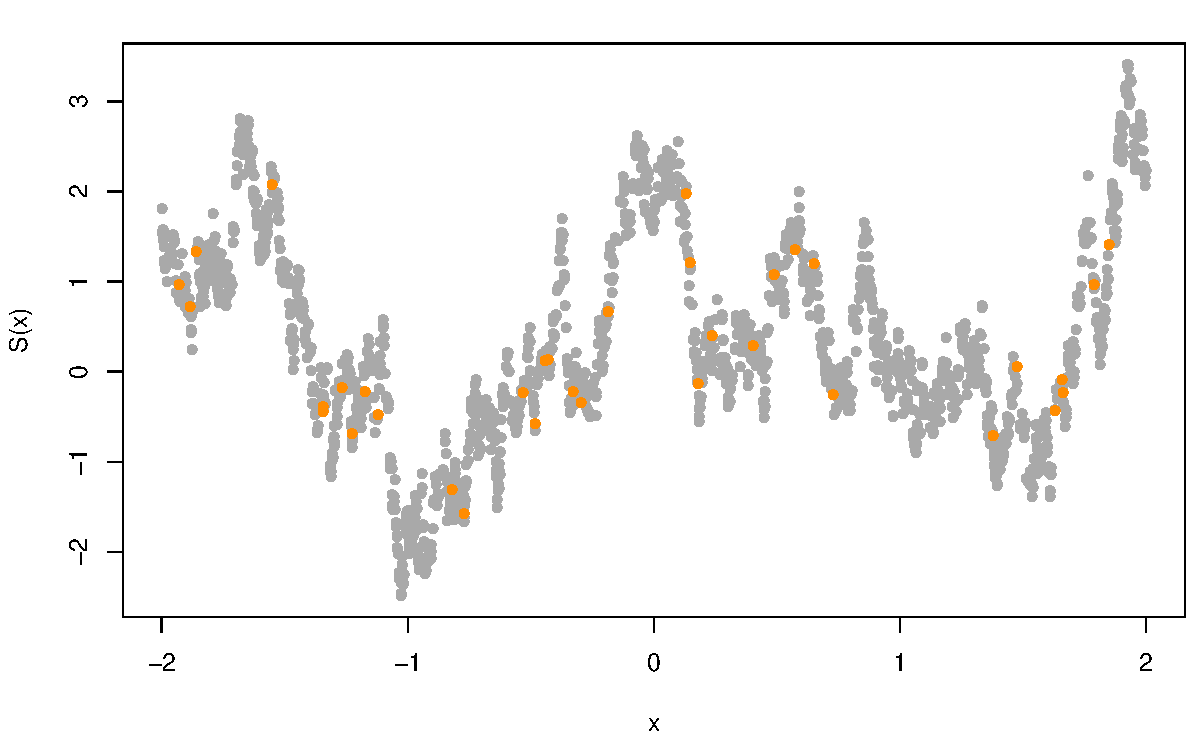
\includegraphics[width=0.7\linewidth]{figures/one-dim-gp-exp} }\\\subfloat[平稳空间高斯过程 $S(x)$ 的协方差函数是幂二次指数型,均值向量为 $\mathbf{0}$,协方差参数 $\sigma^2 = 1$,$\phi = 0.15$,$\kappa=2$\label{fig:one-dim-gp2}]{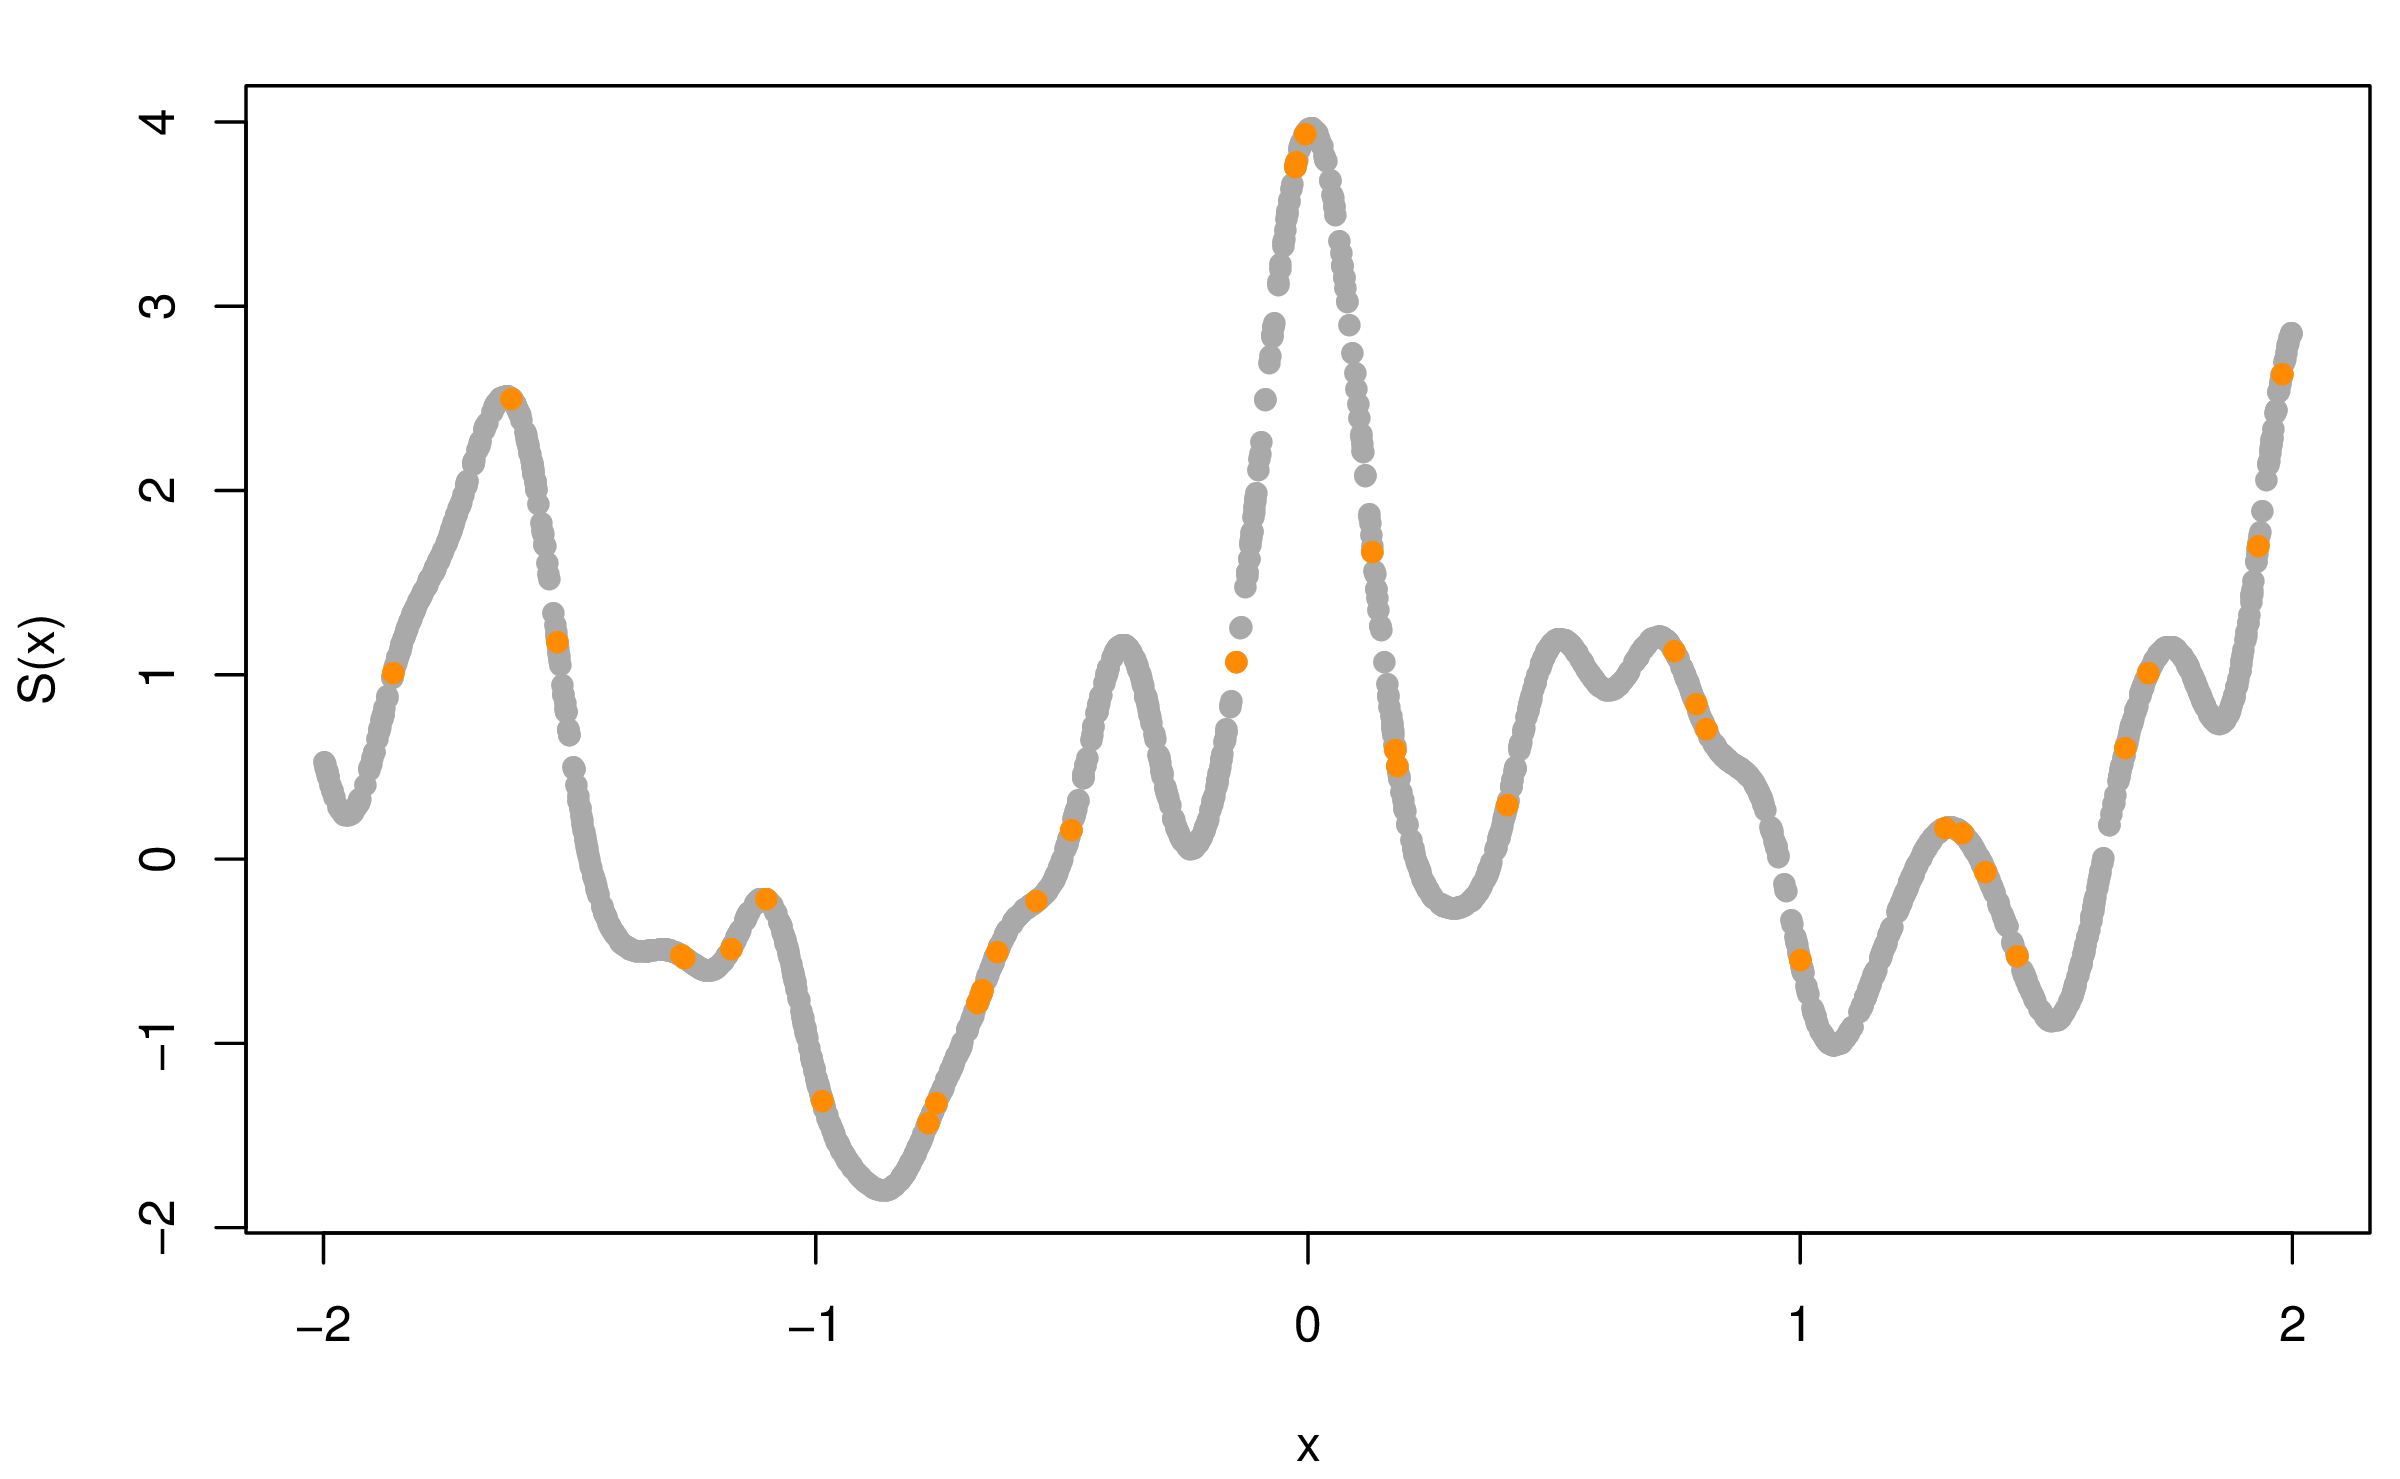
\includegraphics[width=0.7\linewidth]{figures/one-dim-gp-exp-quad} }

}

\caption{模拟一维平稳空间高斯过程,协方差函数分别为指数型
\eqref{eq:cov-exp} 和幂二次指数型 \eqref{eq:cov-exp-quad},均值为
\(\mathbf{0}\),协方差参数
\(\sigma^2 = 1\),\(\phi = 0.15\),横坐标表示采样的位置,纵坐标是目标值
\(S(x)\),图中 2000
个灰色点表示服从相应随机过程的随机数,橘黄色点是从中随机选择的 36 个点。}\label{fig:one-dim-gp}
\end{figure}








根据定理
\ref{thm:stationary-mean-square-properties},指数型协方差函数的平稳高斯过程在原点连续但是不可微,而幂二次指数型协方差函数在原点无穷可微,可微性越好图像上表现越光滑,对比图
\ref{fig:one-dim-gp} 的两个子图, 可以看出,在协方差参数
\(\sigma^2 = 1\),\(\phi = 0.15\) 相同的情况下,\(\kappa\) 越大越光滑。

\hypertarget{sim-two-gp}{%
\subsection{二维平稳空间高斯过程}\label{sim-two-gp}}

二维情形下,在规则平面上模拟平稳高斯过程
\(\mathcal{S} = S(x), x \in \mathbb{R}^2\), 其均值向量为零向量
\(\mathbf{0}\), 协方差函数为指数型 (见公式 \eqref{eq:cov-exp})
,协方差参数 \(\phi = 1, \sigma^2 = 1\)。在单位平面区域为
\([0,1] \times [0,1]\)
模拟服从上述二维空间平稳高斯过程,不妨将此区域划分为 \(6 \times 6\)
的小网格,而每个格点作为采样的位置,共计
36个采样点,在这些采样点上的观察值即为目标值 \(S(x)\)。

类似本章第 \ref{sim-one-gp} 节模拟一维平稳空间过程的步骤,
首先根据采样点位置坐标和协方差函数 \eqref{eq:cov-exp-quad}
计算得目标空间过程的 \(\mathcal{S}\) 协方差矩阵 \(G\),然后使用 R 包
\textbf{MASS} 提供的 \texttt{mvrnorm} 函数产生多元正态分布随机数,与
\ref{sim-one-gp} 节不同的是这里采用特征值分解,即
\(G = L\Lambda L^{\top}\),与 Cholesky
分解相比,特征值分解更稳定些,但是 Cholesky 分解更快,Stan
即采用此法,后续过程与一维模拟一致。模拟获得的随机数用图
\ref{fig:sim-two-gp} 表示, 格点上的值即为平稳空间高斯过程在该点的取值
(为方便显示,已四舍五入保留两位小数)。

\begin{figure}

{\centering \subfloat[在单位区域的网格点上采样\label{fig:sim-two-gp1}]{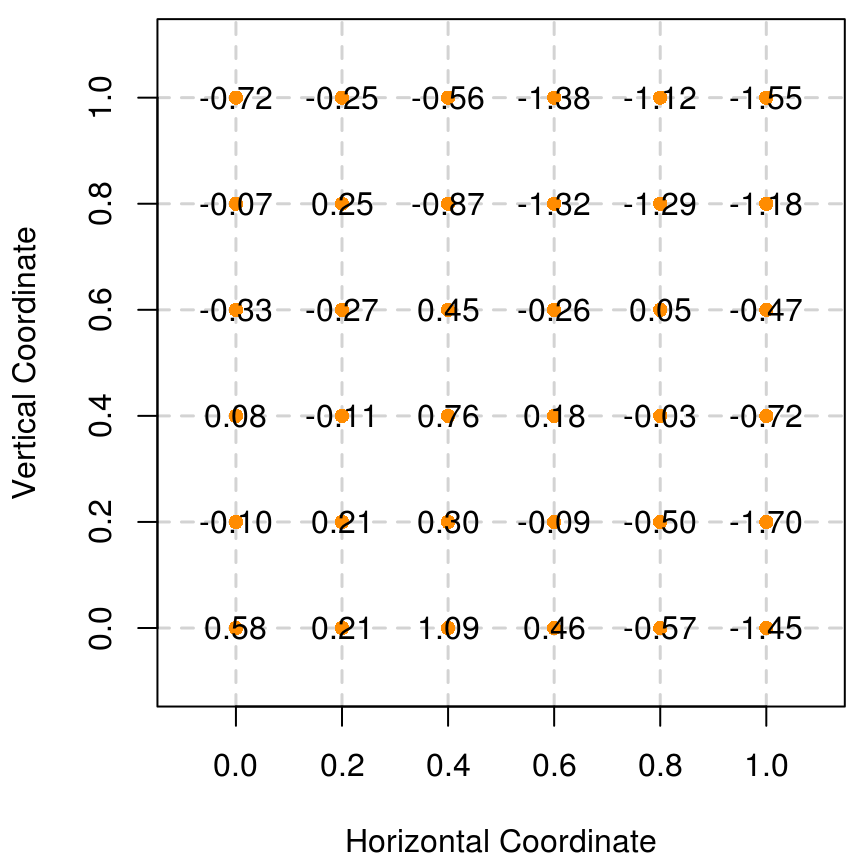
\includegraphics[width=0.45\linewidth]{04-simulations_files/figure-latex/sim-two-gp-1} }\subfloat[在单位区域上随机采样\label{fig:sim-two-gp2}]{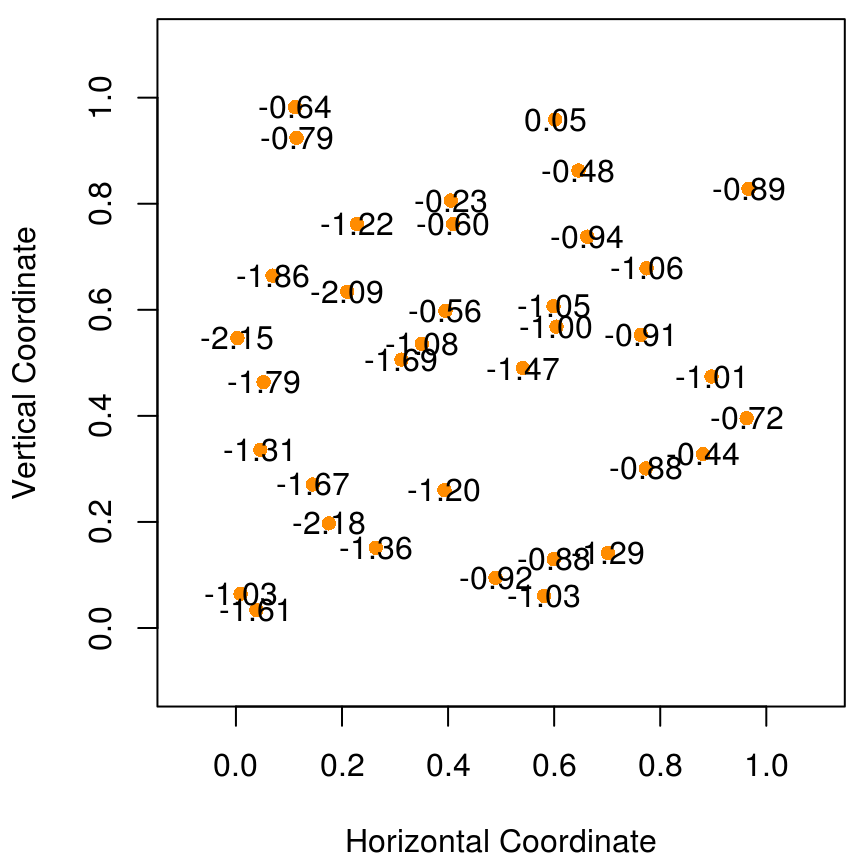
\includegraphics[width=0.45\linewidth]{04-simulations_files/figure-latex/sim-two-gp-2} }

}

\caption{模拟二维平稳空间高斯过程,自相关函数为指数形式,水平方向为横坐标,垂直方向为纵坐标,图中的橘黄色点是采样的位置,其上的数字是目标值 $S(x)$}\label{fig:sim-two-gp}
\end{figure}

同 \ref{sim-one-gp} 节,二维平稳空间高斯过程 \(S(x)\)
的协方差函数也可以为更一般的梅隆型,如公式 \eqref{eq:exp-matern} 所示。

\begin{equation}
\rho(u) = \sigma^2 \{ 2^{\kappa -1} \Gamma(\kappa) \}^{-1}( u/\phi )^{\kappa} \mathcal{K}_{\kappa}( u / \phi ) \label{eq:exp-matern}
\end{equation}

\noindent 且在区域 \([0,1] \times [0,1]\) 上也可以随机采点,如图
\ref{fig:sim-two-gp} 的右子图所示。

模拟平稳空间高斯过程的其它 R 包实现方法: Paulo J. Ribeiro Jr.~和 Peter
J. Diggle 开发了 \textbf{geoR} 包 \citep{geoR2001},提供的 \texttt{grf}
函数除了实现 Cholesky
分解,还实现了奇异值分解,特征值分解协方差矩阵的算法。当采样点不太多时,Cholesky
分解已经足够好,下面的第 \ref{sim-sglmm}
节对平稳空间高斯过程的数值模拟即采用此法,当采样点很多,为了加快模拟的速度,可以选用
Martin Schlather 等开发的 \textbf{RandomFields} 包
\citep{RandomFields2015},内置的 \texttt{GaussRF}
函数实现了用高斯马尔科夫随机场近似平稳空间高斯过程的算法,此外,Håvard
Rue 等 (2009年) \citep{Rue2009}
也实现了从平稳高斯过程到高斯马尔科夫随机场的近似算法,开发了更为高效的
INLA 程序库 \citep{INLA2015},其内置的近似程序得到了广泛的应用
\citep{Virgilio2018, Blangiardo2015, Faraway2018}。

\hypertarget{sim-sglmm}{%
\section{空间广义线性混合效应模型}\label{sim-sglmm}}

\hypertarget{sim-binomal-sglmm}{%
\subsection{响应变量服从二项分布}\label{sim-binomal-sglmm}}

响应变量服从二项分布
\(Y_{i} \sim \mathrm{Binomal}(m_{i},p(x_{i}))\),在位置 \(x_i\)
处,以概率 \(p(x_i)\) 重复抽取了 \(m_i\) 个样本,总样本数
\(M=\sum_{i=1}^{N}m_i\),\(N\)
是采样点的个数,二项空间广义线性混合效应模型为
\eqref{eq:binom-SGLMM},联系函数为
\(g(\mu_i) = \log\{\frac{p(x_i)}{1-p(x_i)}\}\),\(S(x)\) 是均值为
\(\mathbf{0}\),协方差函数为
\(\mathrm{Cov}(S(x_i),S(x_j)) = \sigma^2 \big\{2^{\kappa-1}\Gamma(\kappa)\big\}^{-1}(u/\phi)^{\kappa}K_{\kappa}(u/\phi), \kappa = 0.5\)
的平稳空间高斯过程。

\begin{equation}
g(\mu_i) = \log\{\frac{p(x_i)}{1-p(x_i)}\} = \alpha + S(x_i) \label{eq:binom-SGLMM}
\end{equation}

固定效应参数 \(\alpha = 0\),协方差参数记为
\(\boldsymbol{\theta} = (\sigma^2, \phi) = (0.5, 0.2)\),采样点数目为
\(N = 64\),每个采样点抽取的样本数
\(m_i = 4, i = 1, 2, \ldots, 64\)。首先模拟平稳空间高斯过程
\(S(x)\),在单位区域 \([0,1] \times [0,1]\) 划分为 \(8 \times 8\)
的网格,格点选为采样位置,用 \textbf{geoR} 包提供的 \texttt{grf}
函数产生协方差参数为
\(\boldsymbol{\theta} = (\sigma^2,\phi) = (0.5, 0.2)\)
的平稳空间高斯过程,由公式 \eqref{eq:binom-SGLMM} 可知
\(p(x_i) = \exp(S(x_i))/(1 + \exp(S(x_i)))\),
即每个格点处二项分布的概率值,然后依此概率,由 \texttt{rbinom}
函数产生服从二项分布的观察值 \(Y_i\),\(Y_i\) 的取值范围为
\(0, 1, 2, 3, 4\),模拟的数据集可以用图
\ref{fig:binom-without-nugget-geoRglm} 直观表示。

\begin{figure}

{\centering 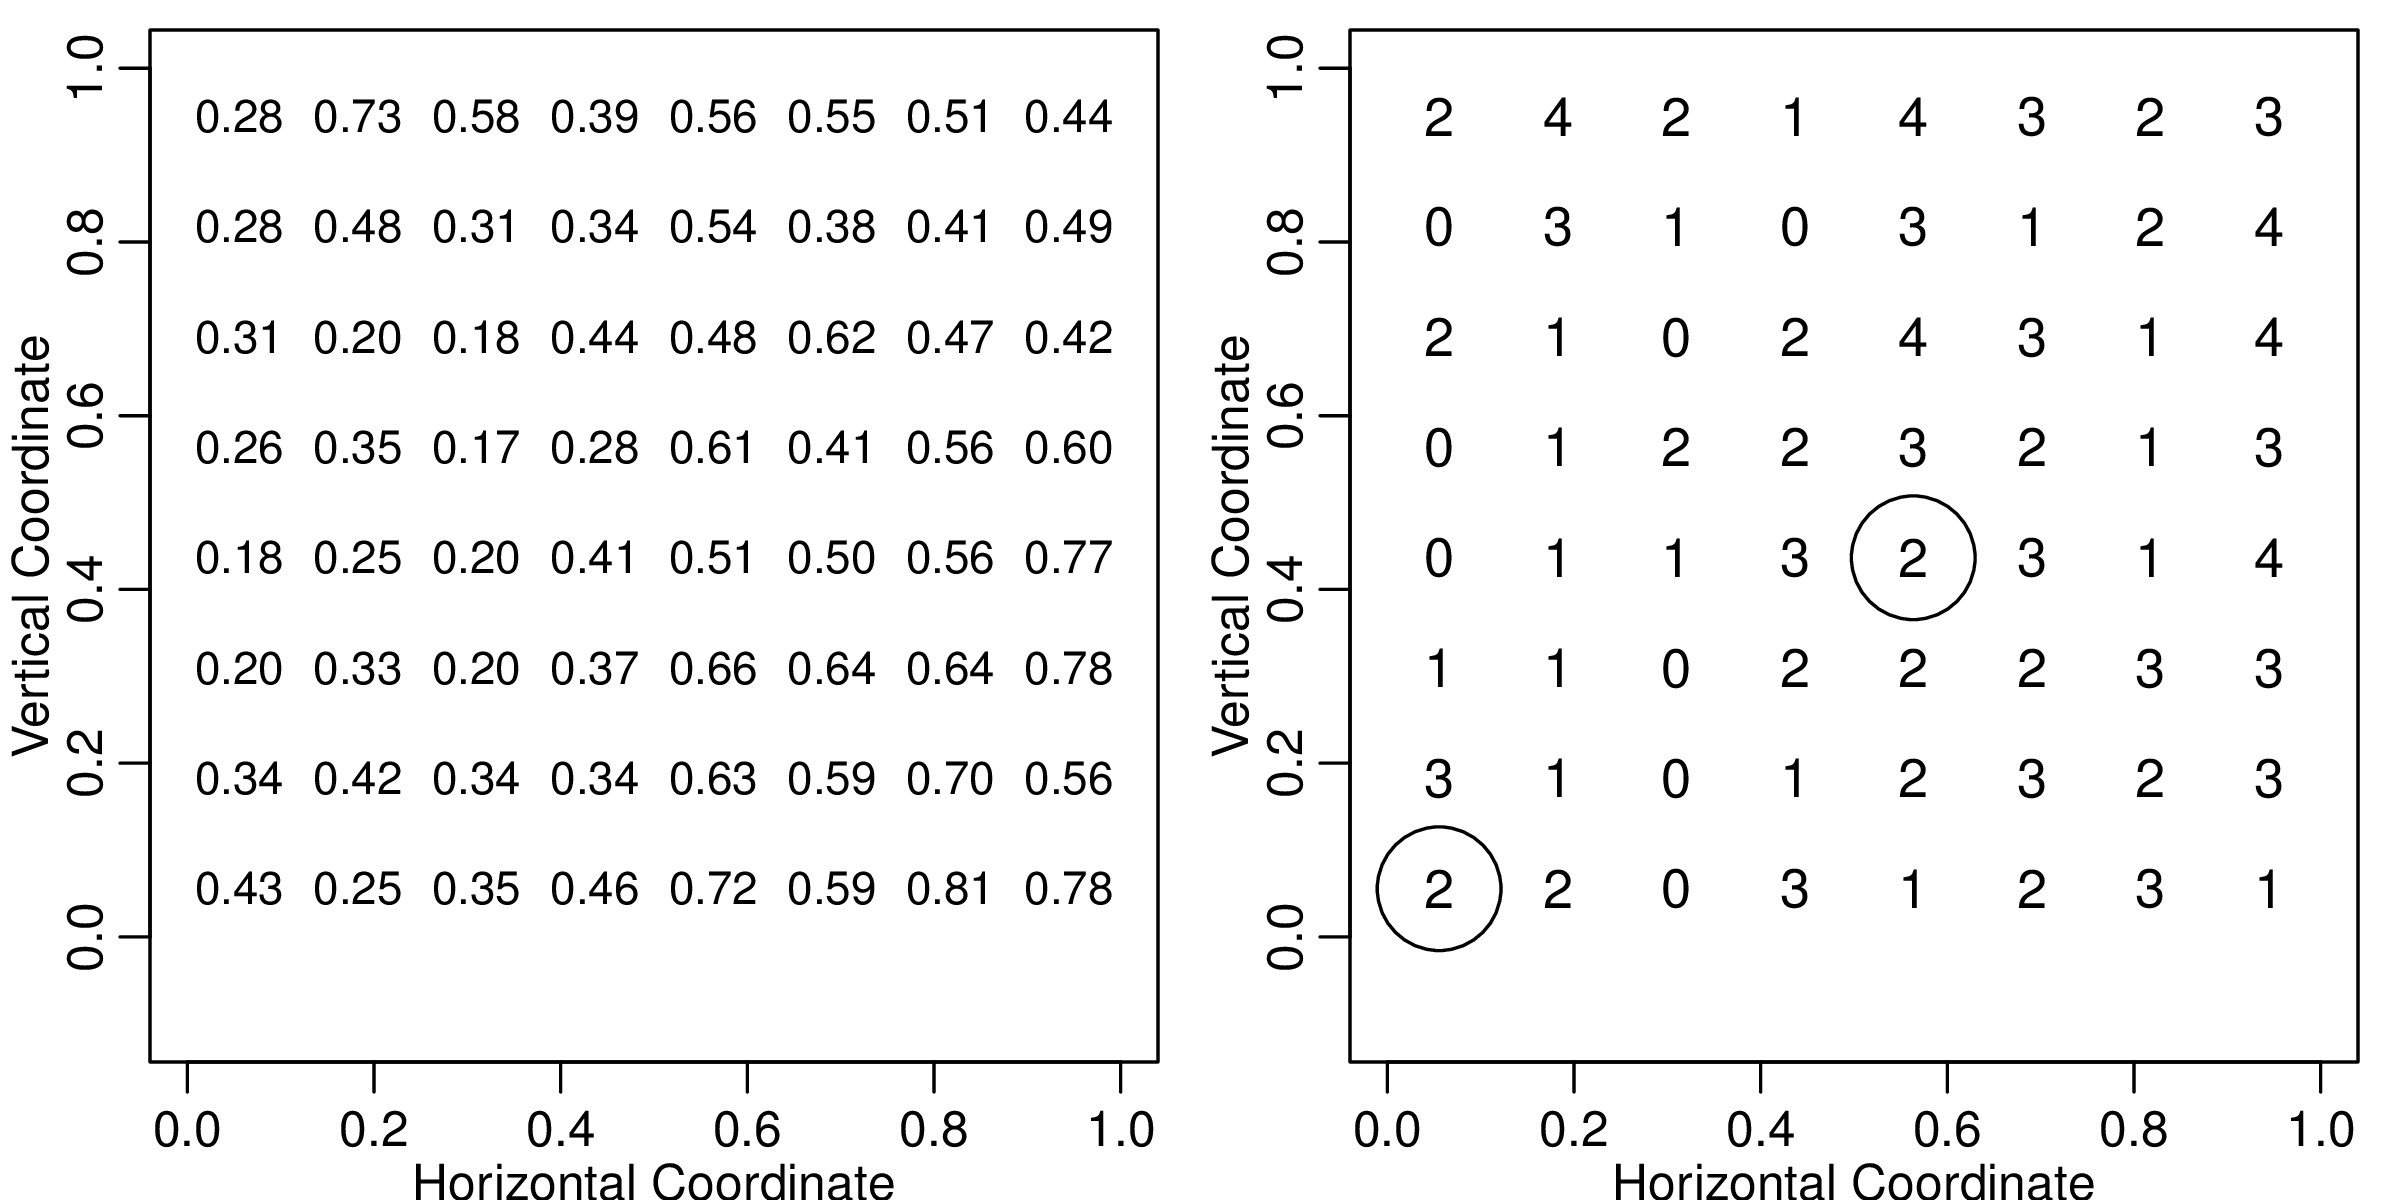
\includegraphics[width=0.9\linewidth]{figures/binom-without-nugget-geoRglm} 

}

\caption{左图表示二维规则平面上的平稳空间高斯过程,格点是采样点的位置,其上的数字是 $p(x)$ 的值,已经四舍五入保留两位小数,右图表示观察值 $Y$ 随空间位置的变化,格点上的值即为观察值 $Y$,图中的两个圈分别是第1个(左下)和第29个(右上)采样点}\label{fig:binom-without-nugget-geoRglm}
\end{figure}

基于 Langevin-Hastings 采样器实现的马尔科夫链蒙特卡罗算法,参数
\(\alpha\) 的先验分布选均值为 0,方差为 1 的标准正态分布,参数 \(\phi\)
的先验分布选期望为 0.2 的指数分布,参数 \(\sigma^2\)
的先验分布是非中心的逆卡方分布,其非中心化参数为 0.5,自由度为
5,各参数的先验选择来自 Ole F. Christensen 和 Peter J. Ribeiro Jr.
(2002年) \citep{geoRglm2002}。Langevin-Hastings 算法运行 110000
次迭代,前 10000 次迭代用作热身 (warm-up),后 10 万次迭代里间隔 100
次迭代采样,获得关于参数 \(\alpha,\phi,\sigma^2\)
的后验分布的样本,样本量是1000。

\begin{align}
\alpha   & \sim \mathcal{N}(0,1) \\
\phi     & \sim \mathrm{Exp}(0.2) \\
\sigma^2 & \sim \mathrm{Inv-}\chi^2(5,0.5)
\end{align}

\begin{longtable}[]{@{}lrrrrrrrr@{}}
\caption{\label{tab:MCLH-vs-NUTS} Langevin-Hastings 算法与 NUTS
算法的数值模拟比较,模型参数 \(\alpha,\phi,\sigma^2\)
的估计值(后验分布的均值)、方差(后验分布的方差)和 5
个分位点(后验分布的 5 个分位点),采样点数目分别考虑了
\(N = 36, 64, 81, 100\) 的情况,括号内为相应参数的真值}\tabularnewline
\toprule
& mean & var & 2.5\% & 25\% & 50\% & 75\% & 97.5\% & N\tabularnewline
\midrule
\endfirsthead
\toprule
& mean & var & 2.5\% & 25\% & 50\% & 75\% & 97.5\% & N\tabularnewline
\midrule
\endhead
\(\alpha\) & -0.354(0) & 0.079 & -0.938 & -0.524 & -0.361 & -0.173 &
0.215 & 36\tabularnewline
\(\phi\) & 0.121(0.2) & 0.006 & 0.005 & 0.055 & 0.110 & 0.180 & 0.285 &
36\tabularnewline
\(\sigma^2\) & 0.683(0.5) & 0.147 & 0.215 & 0.408 & 0.596 & 0.850 &
1.667 & 36\tabularnewline
\(\alpha\) & 0.003(0) & 0.089 & -0.596 & -0.169 & 0.013 & 0.179 & 0.609
& 64\tabularnewline
\(\phi\) & 0.194(0.2) & 0.004 & 0.070 & 0.145 & 0.195 & 0.250 & 0.295 &
64\tabularnewline
\(\sigma^2\) & 0.656(0.5) & 0.096 & 0.254 & 0.449 & 0.592 & 0.781 &
1.453 & 64\tabularnewline
\(\beta\) & -0.155(0) & 0.044 & -0.565 & -0.284 & -0.156 & -0.03 & 0.273
& 81\tabularnewline
\(\phi\) & 0.116(0.2) & 0.006 & 0.005 & 0.055 & 0.105 & 0.17 & 0.280 &
81\tabularnewline
\(\sigma^2\) & 0.468(0.5) & 0.057 & 0.180 & 0.311 & 0.414 & 0.56 & 1.129
& 81\tabularnewline
\bottomrule
\end{longtable}

参数 \(\alpha,\phi,\sigma^2\)
的贝叶斯估计没有显式表达式,通常用后验分布的均值作为参数的估计,
估计的精度或者说好坏用后验分布的方差衡量,而均方误差在参数估计取后验均值时,就是后验方差,所以表
\ref{tab:MCLH-vs-NUTS} 不再提供估计的均方误差值,而是提供了 5
个后验分布的分位点,在 95\% 的置信水平下,样本分位点 0.025 和 0.975
的值组成了置信区间的上下界。64 个采样点处 \(p(x_i), i = 1, \ldots, 64\)
的后验分布的均值、方差、标准差和 5个分位点见附表
\ref{tab:LH-binom-SGLMM}

\hypertarget{possion-sglmm}{%
\subsection{响应变量服从泊松分布}\label{possion-sglmm}}

响应变量 \(Y\) 服从泊松分布,即
\(Y_i \sim \mathrm{Possion}(\lambda(x_{i}))\),泊松空间广义线性混合效应模型
\eqref{eq:pois-SGLMM}

\begin{equation}
g(\mu_i) = \log(\lambda(x_i)) = \alpha + S(x_i) \label{eq:pois-SGLMM}
\end{equation}

\noindent 其中,\(S(x)\) 是平稳空间高斯过程,其均值为
\(\mathbf{0}\),协方差函数为
\(\mathrm{Cov}(S(x_i),S(x_j)) = \sigma^2 \big\{2^{\kappa-1}\Gamma(\kappa)\big\}^{-1}(u/\phi)^{\kappa}K_{\kappa}(u/\phi)\),联系函数
\(g(\mu_i) = \log\{\lambda(x_{i})\}\)。

类似 \ref{sim-binomal-sglmm} 小节产生随机数的过程,

\begin{longtable}[]{@{}lrrrrrrrrr@{}}
\caption{\label{tab:Pois-MCLV-vs-NUTS} 模型参数真值设置为
\(\alpha = 0.5, \phi = 0.2, \sigma^2 = 2.0, \kappa = 1.5\),采样点数目分别为
\(N=36,64,100\)}\tabularnewline
\toprule
& true & mean & var & 2.5\% & 25\% & 50\% & 75\% & 97.5\% &
N\tabularnewline
\midrule
\endfirsthead
\toprule
& true & mean & var & 2.5\% & 25\% & 50\% & 75\% & 97.5\% &
N\tabularnewline
\midrule
\endhead
\(\alpha\) & 0.5 & 0.527 & 0.418 & -0.759 & 0.189 & 0.514 & 0.855 &
1.864 & 36\tabularnewline
\(\phi\) & 0.2 & 0.401 & 0.052 & 0.100 & 0.240 & 0.360 & 0.520 & 0.960 &
36\tabularnewline
\(\sigma^2\) & 2.0 & 1.311 & 0.660 & 0.365 & 0.766 & 1.081 & 1.584 &
3.562 & 36\tabularnewline
\(\alpha\) & 0.5 & 0.866 & 1.517 & -1.610 & 0.059 & 0.870 & 1.666 &
3.159 & 64\tabularnewline
\(\phi\) & 0.2 & 0.682 & 0.073 & 0.300 & 0.480 & 0.640 & 0.820 & 1.380 &
64\tabularnewline
\(\sigma^2\) & 2.0 & 3.932 & 2.594 & 1.667 & 2.800 & 3.642 & 4.744 &
7.740 & 64\tabularnewline
\(\alpha\) & 0.5 & 0.323 & 0.657 & -1.449 & -0.124 & 0.416 & 0.812 &
1.831 & 100\tabularnewline
\(\phi\) & 0.2 & 0.617 & 0.085 & 0.220 & 0.400 & 0.560 & 0.785 & 1.320 &
100\tabularnewline
\(\sigma^2\) & 2.0 & 1.479 & 0.498 & 0.545 & 0.941 & 1.352 & 1.822 &
3.195 & 100\tabularnewline
\bottomrule
\end{longtable}

\hypertarget{applications}{%
\chapter{数据分析}\label{applications}}

loaloa 和 rongelap 两个真实数据集分别来自 R 包 \textbf{geoRglm} 和
\textbf{PrevMap}, 且被 Peter J. Diggle 等 (2007年)
\citep{Diggle2007ATMP} 和 Ole F Christensen (2004年)
\citep{Christensen2004} 分析过,第 \ref{case-loaloa} 节和第
\ref{case-rongelap}
节给出分析这两个数据集的模型和结果。其中,响应变量服从二项分布的空间广义线性混合效应模型拟合数据集
loaloa, 而响应变量服从泊松分布的空间广义线性混合效应模型拟合数据集
rongelap。

\hypertarget{sptial-random-effects}{%
\section{空间线性混合效应模型}\label{sptial-random-effects}}

Walter W. Stroup 和 P. Stephen Baenziger (1994年) \citep{Stroup1994}
采用完全随机的区组设计研究小麦产量与品种等因素的关系,在 4
块肥力不同的地里都随机种植了 56 种不同的小麦,
实验记录了小麦产量、品种、位置以及土地肥力等数据, José Pinheiro 和
Douglas Bates (2000年) \citep{Pinheiro2000} 将该数据集命名为 Wheat2
,整理后放在 \textbf{nlme} 包里。
这里利用该真实的农业生产数据构建带空间效应的线性混合效应模型,展示诊断和添加空间效应的过程。

图 \ref{fig:yields-block}
按土壤肥力不同分块展示每种小麦的产量,图中暗示数据中有 block
效应,块之间也呈现异方差性,为了更好的表达这种依赖效应,可以基于经纬度信息添加与空间相关的结构
(spatial correlation structures),相应的线性模型

\begin{equation}
y_{ij} = \tau_i + \epsilon_{ij}, \quad \boldsymbol{\epsilon} \sim \mathcal{N}(\mathbf{0},\sigma^2 \boldsymbol{\Lambda}) \label{eq:extended-linear-model}
\end{equation}

其中,\(y_{ij}\) 表示第 \(i\) 种小麦在第 \(j\)
块试验田里的产量,\(i = 1,\ldots,56\),\(j = 1,\ldots,4\)。 \(\tau_i\)
表示第 \(i\) 种小麦的平均产量,\(\epsilon_{ij}\)
是随机误差,假定服从均值为 0,协差阵为 \(\sigma^2 \boldsymbol{\Lambda}\)
的正态分布

\begin{figure}

{\centering 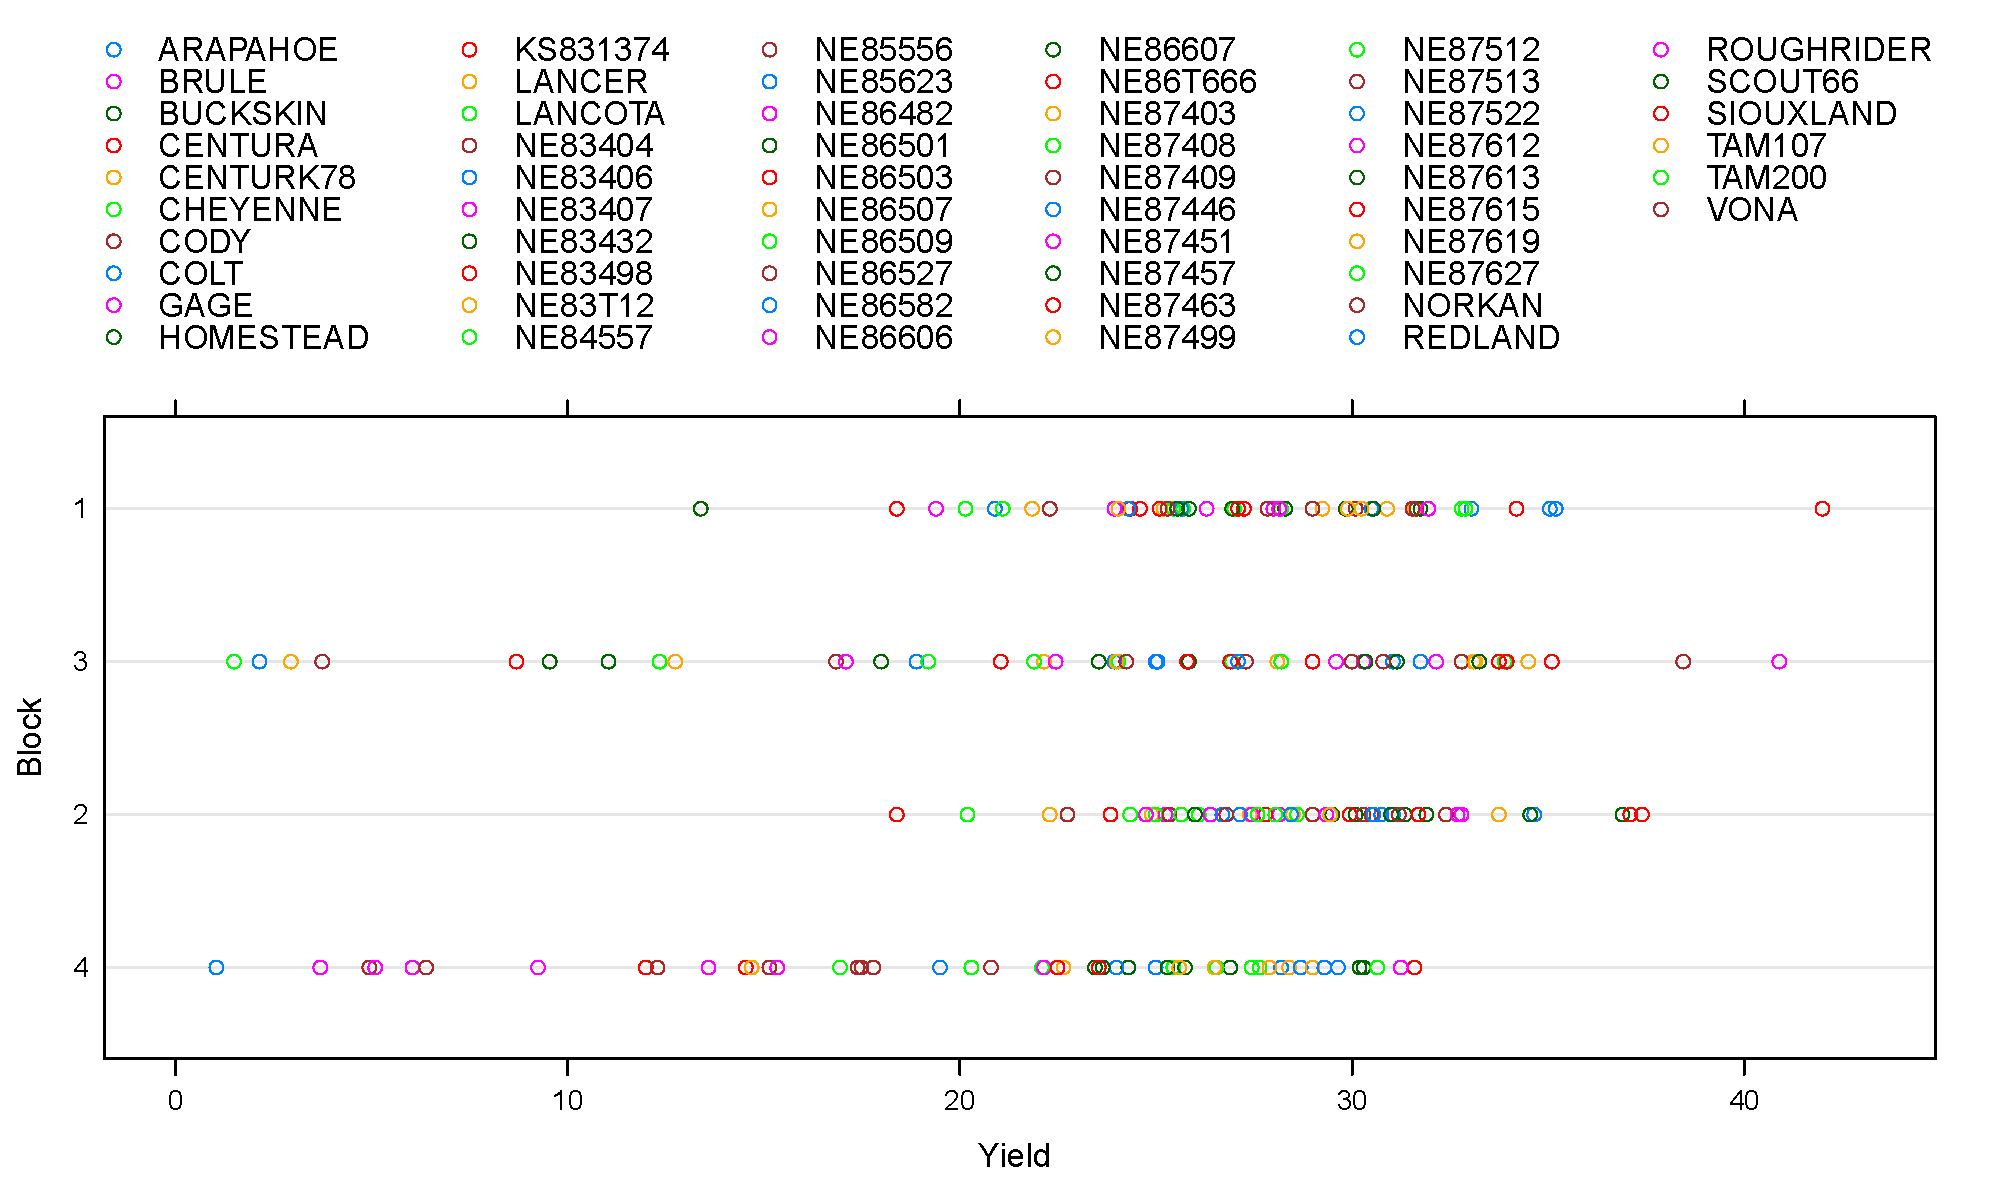
\includegraphics[width=0.9\linewidth]{figures/Yields-Block} 

}

\caption{小麦产量与土壤肥力的关系,图中纵轴表示试验田的4种类型,且土壤肥力强弱顺序是 1 > 2 > 3 > 4,横轴表示小麦产量,每块试验田都种植了 56 种小麦,图中分别以不同的颜色标识,图上方是小麦类型的编号}\label{fig:yields-block}
\end{figure}

探索 \(\boldsymbol{\Lambda}\) 的结构,先假定模型
\eqref{eq:extended-linear-model} 的随机误差是独立且方差齐性的,即
\(\boldsymbol{\Lambda} = \boldsymbol{I}\) 。用如下一行命令拟合模型

\begin{verbatim}
m1 <- gls(yield ~ variety - 1, Wheat2)
\end{verbatim}

拟合残差的样本变差是探索误差中的空间相关性的主要工具,\texttt{Variogram}
方法可以获得 gls 类中的样本变差,即

\begin{verbatim}
Variogram(m1, form = ~latitude + longitude)
\end{verbatim}

图 \ref{fig:yields-variogram}
显示样本变差随空间距离有明显的增长趋势,可见空间相关的结构明显,且块金效应大约是
0.2,样本变差为 1 对应的空间距离是 31
左右。用局部多项式回归方法拟合散点,获得平滑曲线,也可以用局部加权回归散点平滑法来确定初值
\citep{Xie2008COS}。

\begin{figure}

{\centering 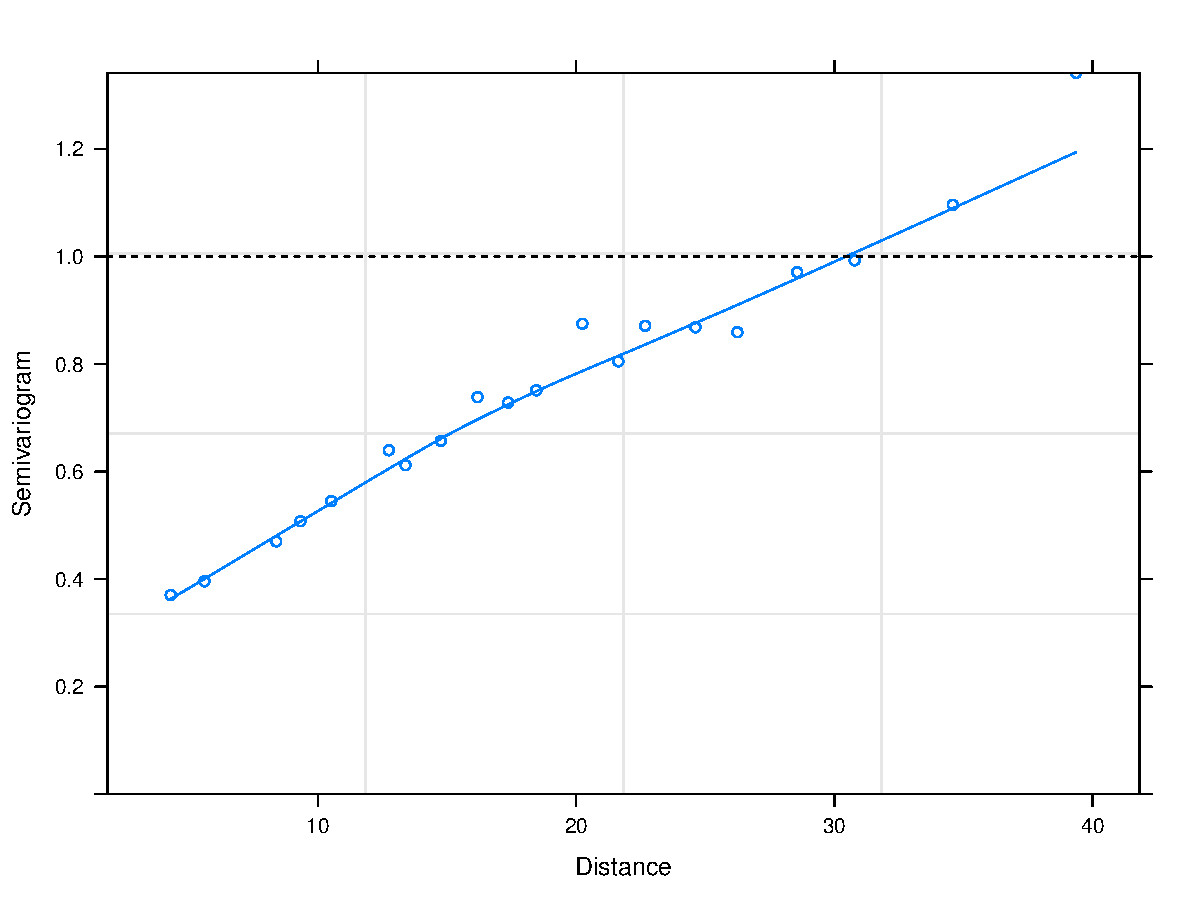
\includegraphics[width=0.7\linewidth]{figures/Yields-Variogram} 

}

\caption{样本变差散点图及局部多项式拟合的变化趋势,横坐标是小麦之间的欧氏距离,纵坐标是样本变差}\label{fig:yields-variogram}
\end{figure}

我们使用球形结构拟合这组数据中的空间结构,位置参数 \(\phi\)
和块金效应的初始值可以从图 \ref{fig:yields-variogram} 获取,其中
\(\phi\) 是样本变差等于 1 时对应的空间距离。拟合模型
\eqref{eq:extended-linear-model}

\begin{verbatim}
m2 <- update(m1, corr = corSpher(
  c(31, 0.2), form = ~latitude + longitude, nugget = TRUE
))
\end{verbatim}

用限制极大似然法做广义最小二乘拟合,空间自相关函数采用球型和二次有理型函数。似然函数对初始值很敏感,去掉样本变差中距离比较远的

\begin{longtable}[]{@{}lrrrrc@{}}
\caption{\label{tab:yields-model-compare} 小麦模型比较}\tabularnewline
\toprule
\begin{minipage}[b]{0.08\columnwidth}\raggedright
\strut
\end{minipage} & \begin{minipage}[b]{0.08\columnwidth}\raggedleft
自相关函数\strut
\end{minipage} & \begin{minipage}[b]{0.18\columnwidth}\raggedleft
\(\hat{\phi}(\phi_0)\)\strut
\end{minipage} & \begin{minipage}[b]{0.20\columnwidth}\raggedleft
\(\hat{\tau}^2(\tau^2_{0})\)\strut
\end{minipage} & \begin{minipage}[b]{0.19\columnwidth}\raggedleft
\(\hat{\sigma}^2(\sigma^2_{0})\)\strut
\end{minipage} & \begin{minipage}[b]{0.09\columnwidth}\centering
log-REML\strut
\end{minipage}\tabularnewline
\midrule
\endfirsthead
\toprule
\begin{minipage}[b]{0.08\columnwidth}\raggedright
\strut
\end{minipage} & \begin{minipage}[b]{0.08\columnwidth}\raggedleft
自相关函数\strut
\end{minipage} & \begin{minipage}[b]{0.18\columnwidth}\raggedleft
\(\hat{\phi}(\phi_0)\)\strut
\end{minipage} & \begin{minipage}[b]{0.20\columnwidth}\raggedleft
\(\hat{\tau}^2(\tau^2_{0})\)\strut
\end{minipage} & \begin{minipage}[b]{0.19\columnwidth}\raggedleft
\(\hat{\sigma}^2(\sigma^2_{0})\)\strut
\end{minipage} & \begin{minipage}[b]{0.09\columnwidth}\centering
log-REML\strut
\end{minipage}\tabularnewline
\midrule
\endhead
\begin{minipage}[t]{0.08\columnwidth}\raggedright
模型 I\strut
\end{minipage} & \begin{minipage}[t]{0.08\columnwidth}\raggedleft
球型\strut
\end{minipage} & \begin{minipage}[t]{0.18\columnwidth}\raggedleft
\(1.515\times 10^{5}(31)\)\strut
\end{minipage} & \begin{minipage}[t]{0.20\columnwidth}\raggedleft
\(5.471\times 10^{-5}(0.2)\)\strut
\end{minipage} & \begin{minipage}[t]{0.19\columnwidth}\raggedleft
466.785\strut
\end{minipage} & \begin{minipage}[t]{0.09\columnwidth}\centering
-533.418\strut
\end{minipage}\tabularnewline
\begin{minipage}[t]{0.08\columnwidth}\raggedright
模型 II\strut
\end{minipage} & \begin{minipage}[t]{0.08\columnwidth}\raggedleft
二次有理型\strut
\end{minipage} & \begin{minipage}[t]{0.18\columnwidth}\raggedleft
\(13.461(13)\)\strut
\end{minipage} & \begin{minipage}[t]{0.20\columnwidth}\raggedleft
\(0.193(0.2)\)\strut
\end{minipage} & \begin{minipage}[t]{0.19\columnwidth}\raggedleft
8.847\strut
\end{minipage} & \begin{minipage}[t]{0.09\columnwidth}\centering
-532.639\strut
\end{minipage}\tabularnewline
\begin{minipage}[t]{0.08\columnwidth}\raggedright
模型 III\strut
\end{minipage} & \begin{minipage}[t]{0.08\columnwidth}\raggedleft
球型\strut
\end{minipage} & \begin{minipage}[t]{0.18\columnwidth}\raggedleft
\(27.457(28)\)\strut
\end{minipage} & \begin{minipage}[t]{0.20\columnwidth}\raggedleft
\(0.209(0.2)\)\strut
\end{minipage} & \begin{minipage}[t]{0.19\columnwidth}\raggedleft
7.410\strut
\end{minipage} & \begin{minipage}[t]{0.09\columnwidth}\centering
-533.931\strut
\end{minipage}\tabularnewline
\bottomrule
\end{longtable}

说明两件事,其一选择合适的自相关函数可以取得好的拟合效果,其二算法对初值很敏感,选择合适的初值很重要。

标准化残差拟合图

\begin{figure}

{\centering \subfloat[检查异方差性\label{fig:model-check1}]{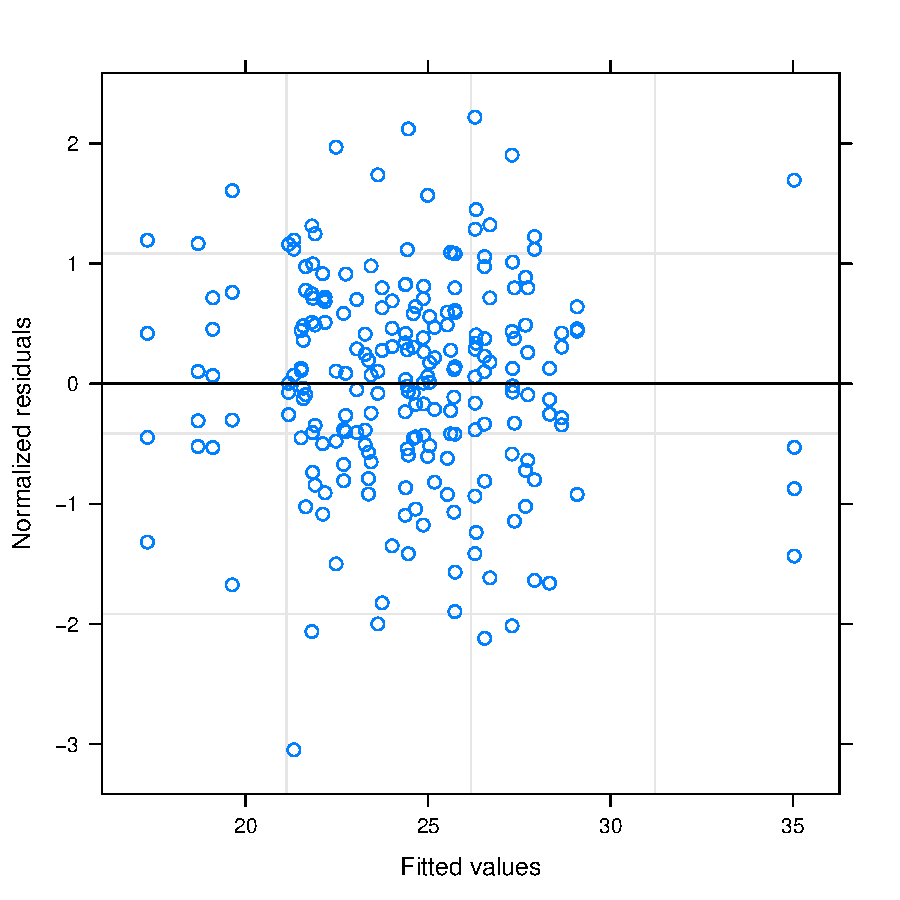
\includegraphics[width=0.4\linewidth]{figures/heteroscedasticity} }\subfloat[检查正态性\label{fig:model-check2}]{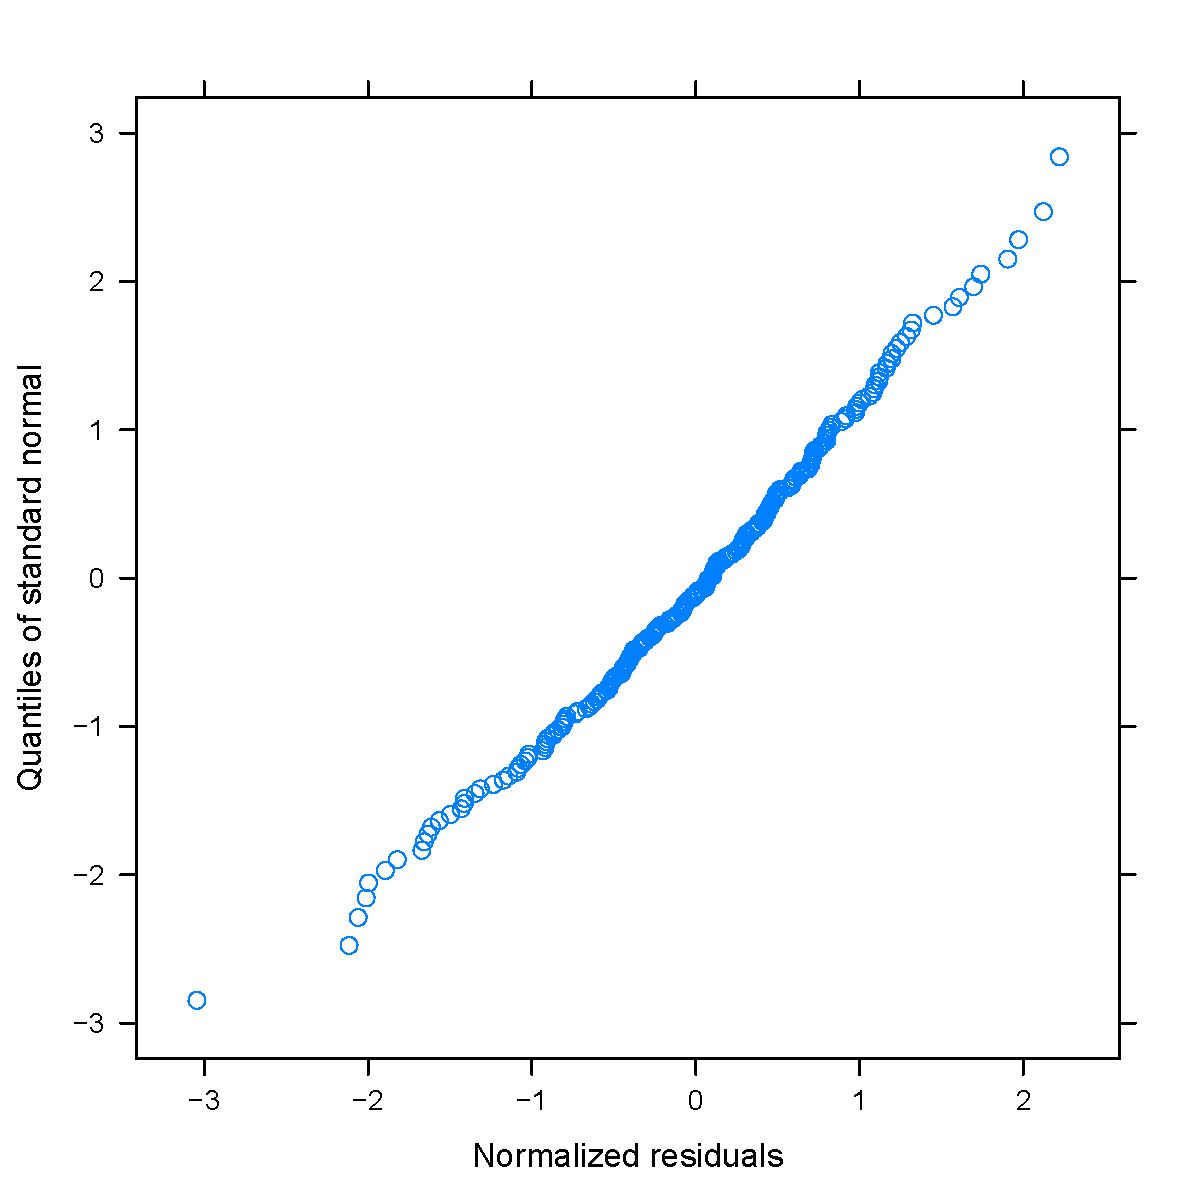
\includegraphics[width=0.4\linewidth]{figures/normality} }

}

\caption{模型诊断}\label{fig:model-check}
\end{figure}

\hypertarget{case-loaloa}{%
\section{喀麦隆及周边地区盘尾丝虫病的空间分布}\label{case-loaloa}}

盘尾丝虫病是由一种可致盲的热带疾病,非洲盘尾丝虫病控制项目 APOC (African
Programme for Onchocerciasis Control) 搜集了 \(N=168\) 个村庄的
\(M = 21938\) 个血液样本,每个村庄抽取的样本量为
\(m_i=\mathrm{NO\_EXAM}\), 其中感染了的 NO\_INF 人, 在该村庄 (坐标
\(x_i\))观察到的感染比例 \(p(x_i) = \mathrm{NO\_INF/NO\_EXAM}\) ,
在村庄 1 公里的范围内添加了周围环境的指标,
有从美国地质调查局获得的海拔信息 ELEVATION (\url{https://www.usgs.gov/})
和卫星在 1999 年至 2001 年间测得的植被绿色度数据 NDVI
(\url{http://free.vgt.vito.be}), NDVI 分四个指标, 分别是所有 NDVI
的平均值 MEAN9901,最大值 MAX9901,最小值 MIN9901,标准差 STDEV9901。
样本采集的区域如图 \ref{fig:loaloa-map} 所示

\begin{figure}

{\centering 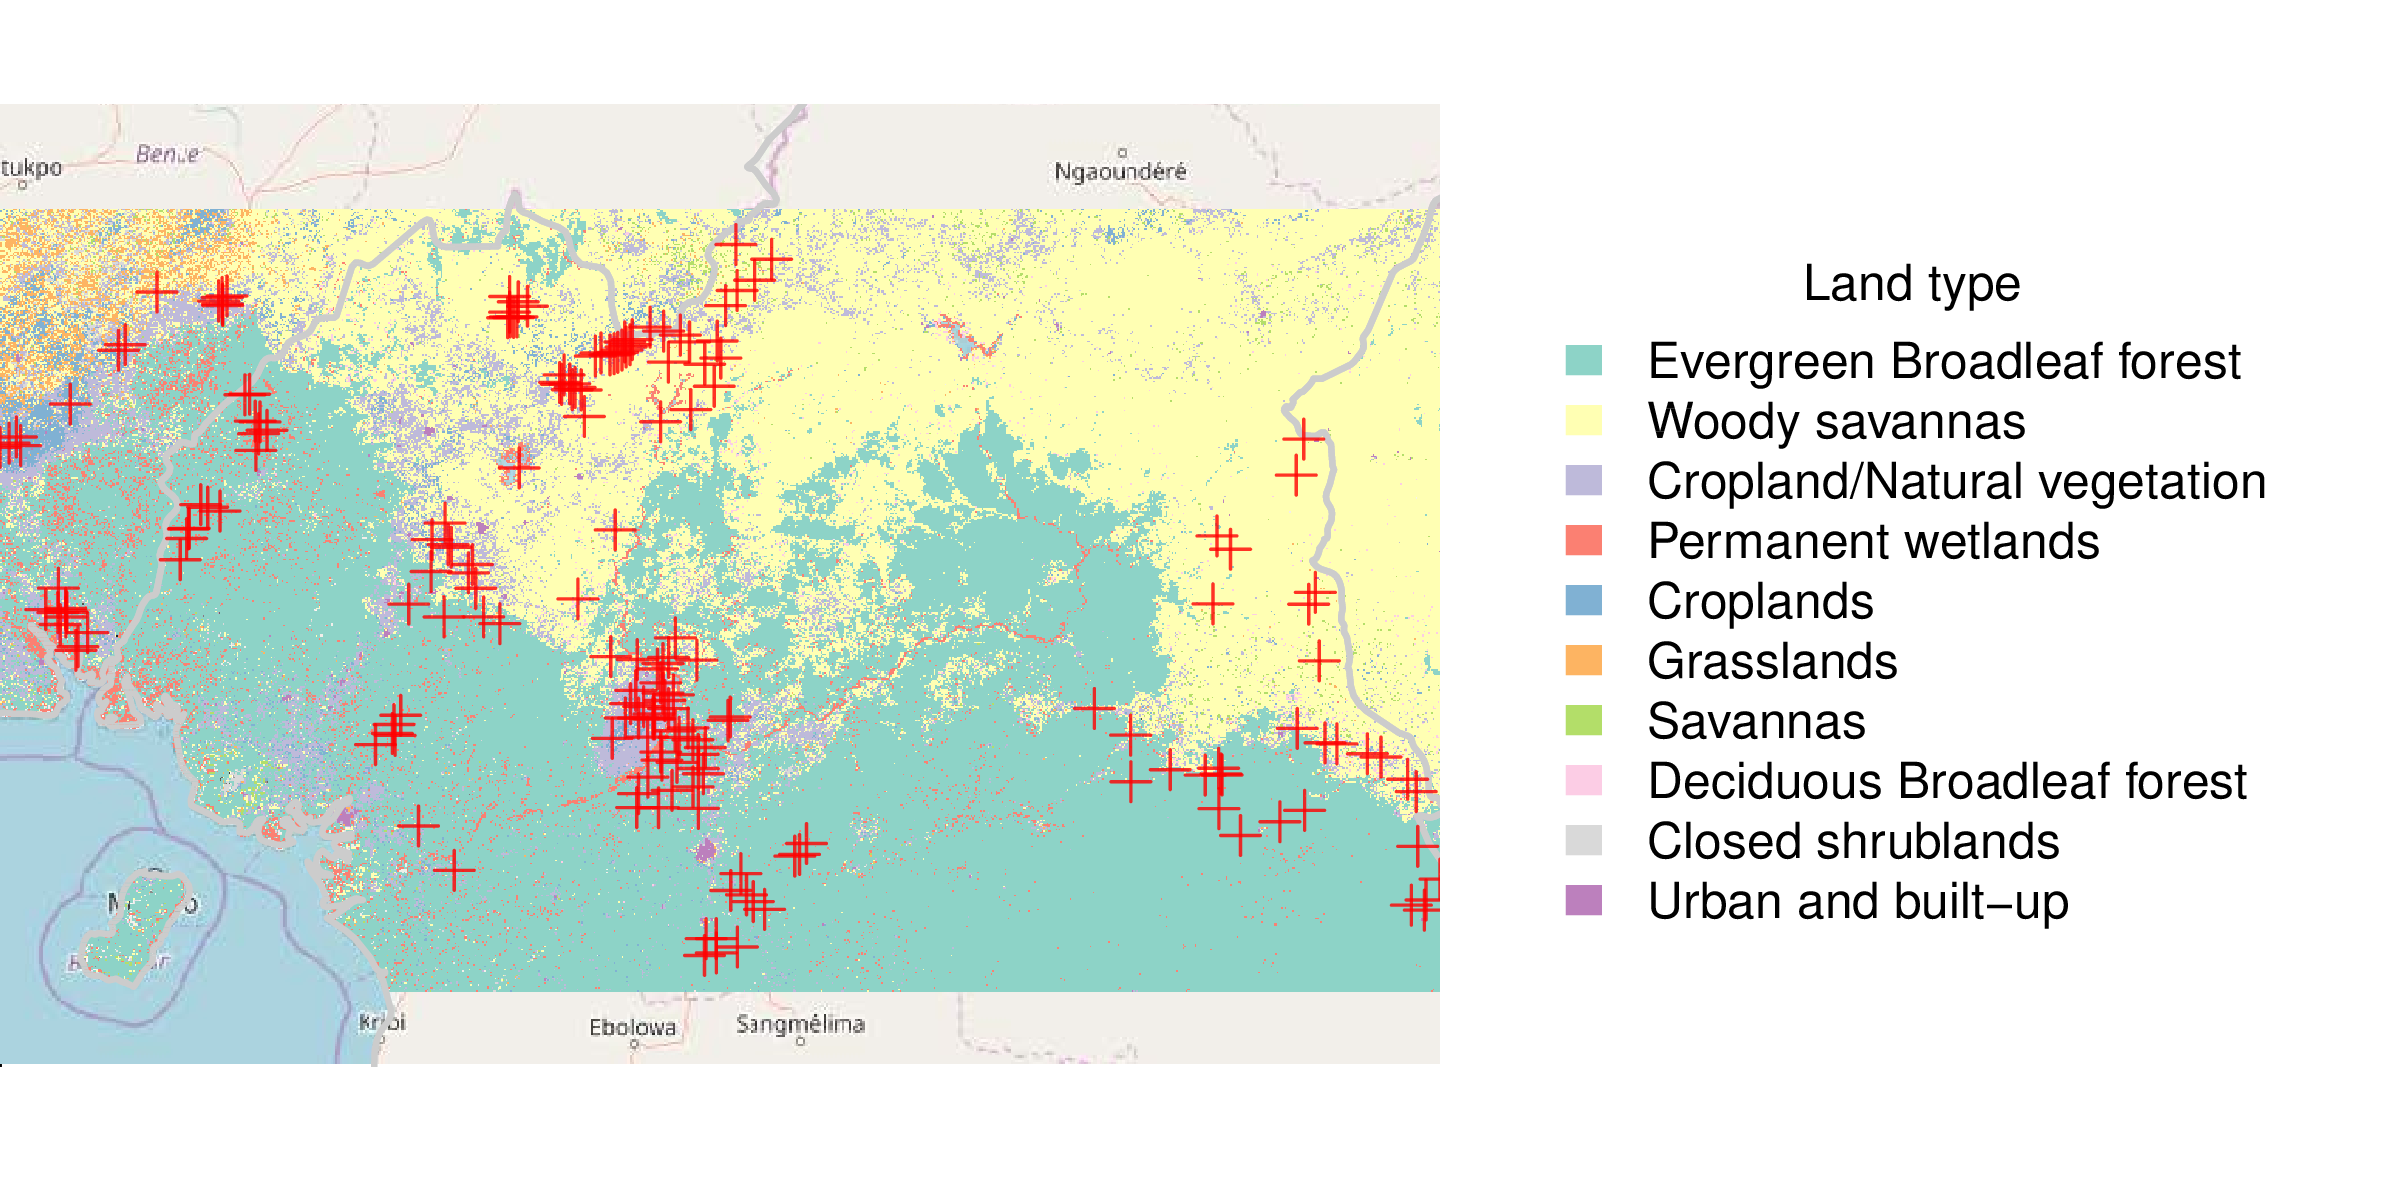
\includegraphics[width=0.9\linewidth]{figures/map-loaloa} 

}

\caption{红色加号标注样本所在的村庄}\label{fig:loaloa-map}
\end{figure}

\noindent 为了分析 loaloa 数据集,我们建立响应变量 \(Y\)
服从二项分布的空间广义线性混合效应模型

\begin{equation*}
\begin{split}
\log\big\{ \frac{ p(x_i)}{ 1-p(x_i)} \big\} = 
               & \beta_{0} + \beta_{1} \times \mathrm{ELEVATION}_{i} + \beta_{2} \times \mathrm{MEAN9901}_{i} + \beta_{3} \times \mathrm{MAX9901}_{i} + \\
               & \beta_{4} \times \mathrm{MIN9901}_{i} +  \beta_{5} \times \mathrm{STDEV9901}_{i} + S(x_{i})
\end{split}
\end{equation*}

\noindent 其中,\(\beta_0\)
是截距,\(\beta_{1},\beta_{2}, \beta_{3},\beta_{4}, \beta_{5}\)
是各指标的系数,\(Y_{i} \sim \mathrm{Binomial}(m_{i},p(x_i))\),平稳空间高斯过程
\(\mathcal{S} = S(x), x = ( \mathrm{LONGITUDE}, \mathrm{LATITUDE}) \in \mathbb{R}^2\)
的均值为 0,自协方差函数为

\[
\mathrm{Cov}(S(x_i),S(x_j)) = \sigma^2 \big\{2^{\kappa-1}\Gamma(\kappa)\big\}^{-1}(u_{ij}/\phi)^{\kappa}K_{\kappa}(u_{ij}/\phi), \kappa = 2
\]

在实际数据分析中,选择一组合适的初始值可以缩短各算法迭代的过程。我们分两步获取
\(\beta = (\beta_{0},\beta_{1},\beta_{2}, \beta_{3},\beta_{4}, \beta_{5})\)
和 \(\boldsymbol{\theta} = (\sigma^2,\phi)\)
的初始值。第一步,离散自协方差函数中的 \(\kappa\),再调用
\textbf{PrevMap} 包中的 \texttt{shape.matern} 函数选择一个
\(\kappa\);第二步,在去掉空间效应 \(S(x)\)
的情况下,以广义线性模型拟合数据得到
\(\beta\)的初始估计值。然后分别使用贝叶斯 MCMC 算法和贝叶斯 STAN-MCMC
算法估计参数
\(\beta = (\beta_{0},\beta_{1},\beta_{2}, \beta_{3},\beta_{4}, \beta_{5})\)
和 \(\boldsymbol{\theta} = (\sigma^2,\phi)\),结果如表
\ref{tab:loaloa-estimation2} 和表 \ref{tab:loaloa-estimation3}所示。

\begin{longtable}[]{@{}cccc@{}}
\caption{\label{tab:loaloa-estimation1}
MCML算法估计模型的参数}\tabularnewline
\toprule
参数 & 估计 & 标准差 & 标准误\tabularnewline
\midrule
\endfirsthead
\toprule
参数 & 估计 & 标准差 & 标准误\tabularnewline
\midrule
\endhead
\(\beta_{0}\) & -11.120 & 1.447 & 8.268e-03\tabularnewline
\(\beta_{1}\) & -0.001 & 3.155e-04 & 1.023e-05\tabularnewline
\(\beta_{2}\) & 13.513 & 2.223 & 4.877e-02\tabularnewline
\(\beta_{3}\) & 1.454 & 2.013 & 3.094e-02\tabularnewline
\(\beta_{4}\) & -0.576 & 1.315 & 1.016e-02\tabularnewline
\(\beta_{5}\) & 11.216 & 5.181 & 5.321e-02\tabularnewline
\(\sigma^2\) & 1.171 & 0.272 & 1.300e-03\tabularnewline
\(\phi\) & 0.486 & 0.353 & 2.344e-03\tabularnewline
\bottomrule
\end{longtable}

通过表 \ref{tab:loaloa-estimation1} 的 P 值,可以看出
\(\beta_{0},\beta_{1},\beta_{2}\) 是显著的,分别对应模型的截距项,海拔
(ELEVATION)和 NDVI 的平均值 (MEAN9901),在这组数据中,刻画 NDVI
指标使用平均值比较能体现村庄周围植被的整体绿色度,而最大值
MAX9901,最小值 MIN9901,标准差 STDEV9901 与影响不显著。

\begin{longtable}[]{@{}cccc@{}}
\caption{\label{tab:loaloa-estimation2} 贝叶斯 MCMC
算法估计模型的参数}\tabularnewline
\toprule
参数 & 估计 & 标准差 & 均方误差\tabularnewline
\midrule
\endfirsthead
\toprule
参数 & 估计 & 标准差 & 均方误差\tabularnewline
\midrule
\endhead
\(\beta_{0}\) & -11.562 & 0.681 & 5.563e-03\tabularnewline
\(\beta_{1}\) & -8.721e-04 & 1.415e-04 & 1.155e-06\tabularnewline
\(\beta_{2}\) & 8.426 & 2.064 & 1.686e-02\tabularnewline
\(\beta_{3}\) & 4.857 & 1.334 & 1.090e-02\tabularnewline
\(\beta_{4}\) & 0.233 & 1.367 & 1.116e-02\tabularnewline
\(\beta_{5}\) & 11.087 & 3.565 & 2.911e-02\tabularnewline
\(\sigma^2\) & 1.096 & 0.170 & 1.390e-03\tabularnewline
\(\phi\) & 3.675 & 0.582 & 4.754e-03\tabularnewline
\bottomrule
\end{longtable}

\begin{longtable}[]{@{}cccc@{}}
\caption{\label{tab:loaloa-estimation3} 贝叶斯 STAN-MCMC
算法估计模型的参数}\tabularnewline
\toprule
参数 & 估计 & 标准差 & 均方误差\tabularnewline
\midrule
\endfirsthead
\toprule
参数 & 估计 & 标准差 & 均方误差\tabularnewline
\midrule
\endhead
\(\beta_{0}\) & -12.878 & 1.460 & 3.515e-03\tabularnewline
\(\beta_{1}\) & -6.596e-04 & 3.188e-04 & 7.733e-07\tabularnewline
\(\beta_{2}\) & 9.647 & 2.136 & 5.222e-03\tabularnewline
\(\beta_{3}\) & 4.380 & 1.993 & 5.026e-03\tabularnewline
\(\beta_{4}\) & -0.102 & 1.159 & 2.822e-03\tabularnewline
\(\beta_{5}\) & 11.216 & 5.539 & 1.343e-02\tabularnewline
\(\sigma^2\) & 1.027 & 0.09 & 2.171e-04\tabularnewline
\(\phi\) & 1.157e-02 & 1.292e-03 & 3.244e-06\tabularnewline
\bottomrule
\end{longtable}

比较表 \ref{tab:loaloa-estimation2} 和表 \ref{tab:loaloa-estimation3},
发现贝叶斯 STAN-MCMC 算法比贝叶斯 MCMC 算法稍好一点,
多半的参数估计的标准差要小一些, 均方误差普遍要小一点。

\hypertarget{case-rongelap}{%
\section{朗格拉普岛核污染浓度的空间分布}\label{case-rongelap}}

Peter J. Diggle 等 (1998年) \citep{Diggle1998}
提出蒙特卡罗极大似然方法估计不带块金效应的响应变量服从泊松分布的空间广义混合效应模型
(见模型 \eqref{eq:rongelap-without-nugget-effect}
)的参数,分析了朗格拉普岛上核污染浓度的空间分布,后来,Ole F Christensen
(2004年) \citep{Christensen2004}
发现该核污染数据集中存在不能被泊松分布解释的残差,因此在 Peter J. Diggle
等 (1998年) \citep{Diggle1998} 的基础上添加了块金效应,见模型
\eqref{eq:rongelap-with-nugget-effect},
同样使用蒙特卡罗极大似然方法估计了模型中的参数。

朗格拉普岛位于南太平洋上,是马绍尔群岛的一部分,二战后,美国在该岛上进行了核武器测试,核爆炸后产生的放射性尘埃笼罩了全岛,目前该岛仍然不适合人类居住,只有经批准的科学研究人员才能登岛,核污染残留浓度是其中一项
\citep{Bordner2016}。rongelap 数据集包含伽马射线在 \(N=157\)
站点不同时间间隔的放射量,伽马射线在时间间隔 units.m 内放射的粒子数目为
y,d1 和 d2 分别为测量坐标。 建立 Poisson-SGLMM 模型

\begin{figure}

{\centering 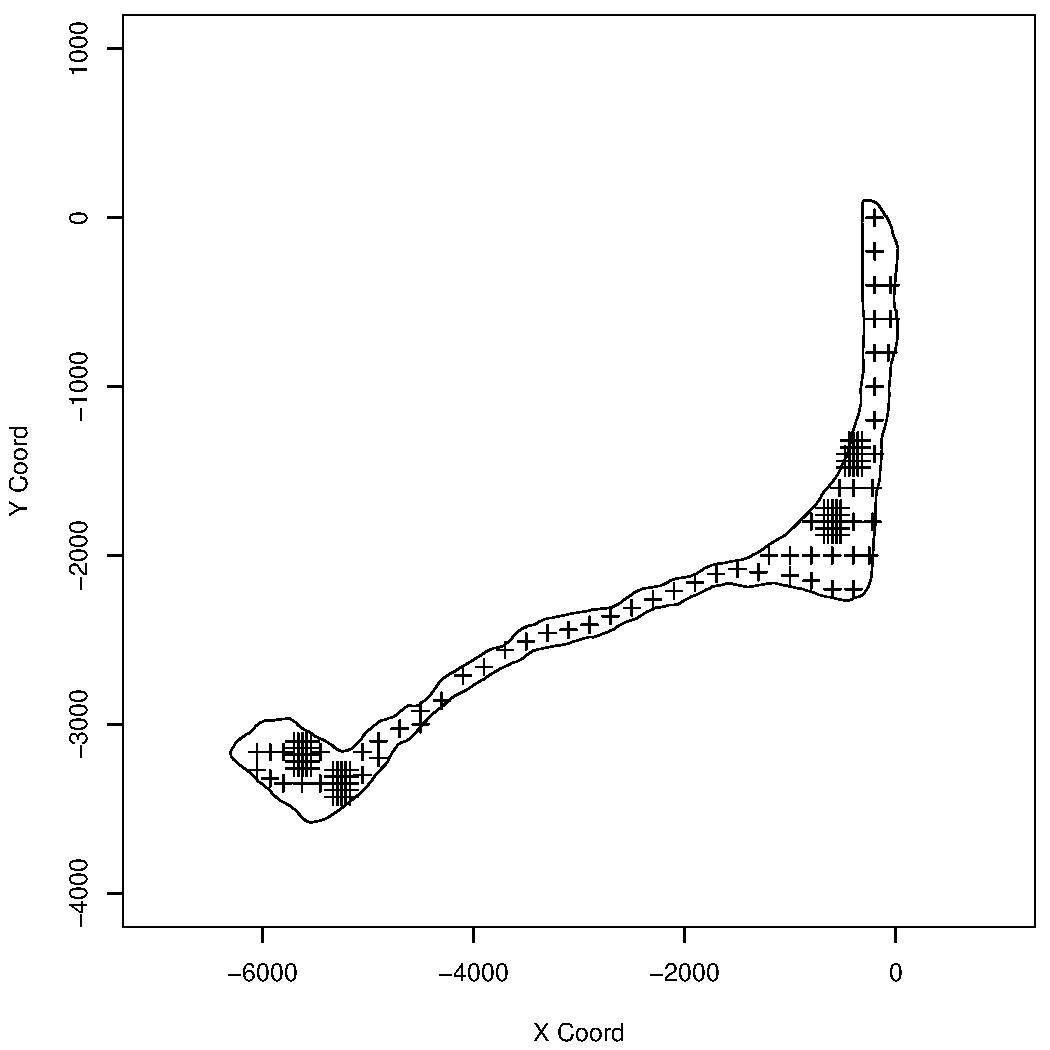
\includegraphics[width=0.7\linewidth]{figures/rongelap-island} 

}

\caption{朗格拉普岛上采样点的位置,加号 + 表示采样的位置}\label{fig:rongelap-dataset}
\end{figure}

\begin{align}
\log\{\lambda(x_{i})\}& =  \beta + S(x_{i}) \label{eq:rongelap-without-nugget-effect}\\
\log\{\lambda(x_{i})\}& =  \beta + S(x_{i}) + Z_{i} \label{eq:rongelap-with-nugget-effect}
\end{align}

\noindent 其中,\(\beta_0\) 是截距, 响应变量
\(Y_{i} \sim \mathrm{Poisson}( \lambda(x_i) )\),平稳空间高斯过程的自协方差函数为
\(\mathsf{Cov}( S(x_i), S(x_j) ) = \sigma^2 \exp( -\|x_i -x_j\|_{2} / \phi )\),\(\mathsf{Var}( Z_{i} ) = \tau^2, i = 1, \ldots, N = 157\)

蒙特卡罗极大似然算法迭代的初值
\(\beta_{0} = 6.2,\sigma^2_{0} = 2.40,\phi_{0} = 340,\tau^2_{rel} = 2.074\),模拟次数为
30000 次,前 10000 次迭代视为预热阶段 (warm-up)
而不用于参数的估计,其后每隔 20
次迭代采一个样本点,存储各模型参数的迭代值,其间模拟条件分布 \([S|y]\)
产生蒙特卡罗马尔科夫链使用了 Langevin-Hastings 算法 \citep{Omiros2003}。

\begin{figure}

{\centering 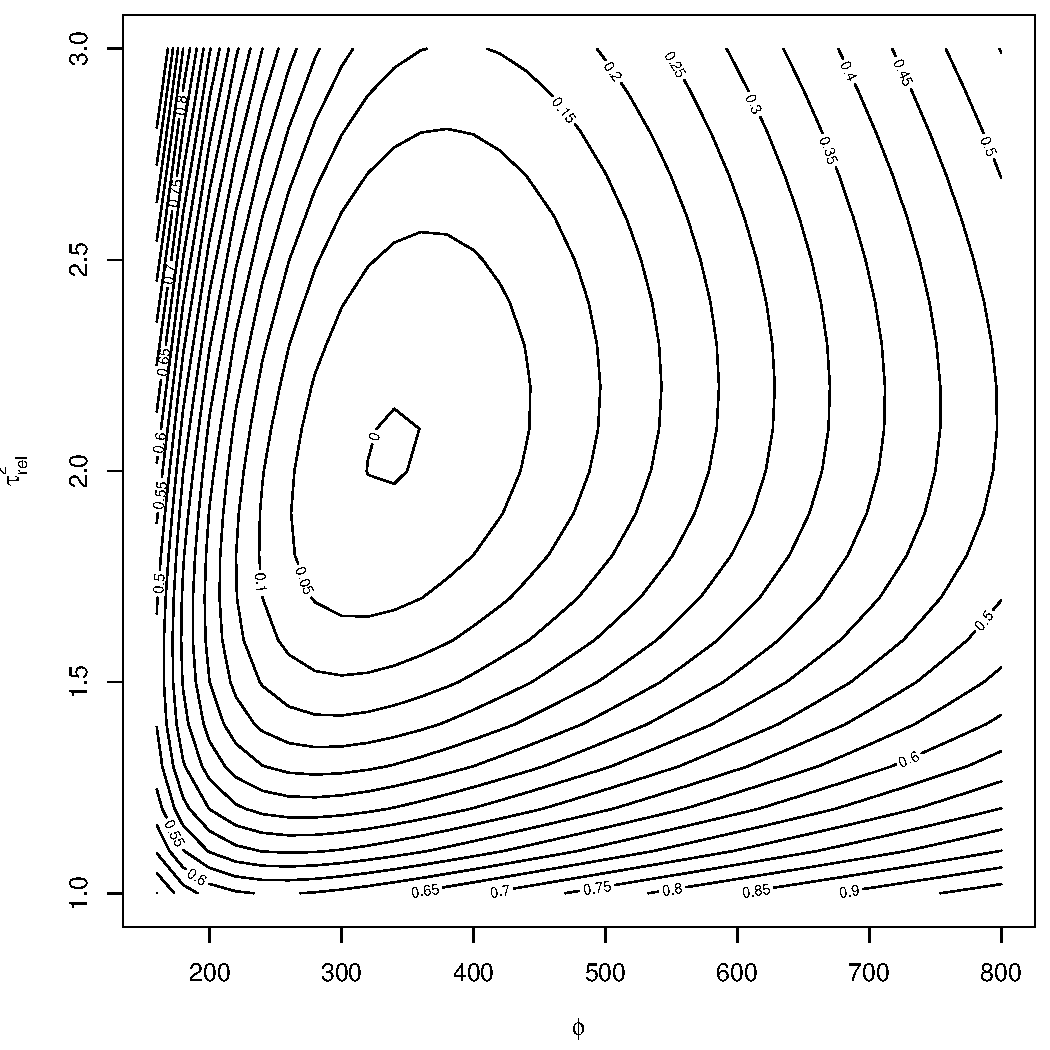
\includegraphics[width=0.7\linewidth]{figures/profile-phitausq} 

}

\caption{关于 \(\phi\) 和相对块金效应
\(\tau^2_{rel} = \tau^2 / \sigma^2\)
的剖面似然函数曲面,平稳空间高斯过程的协方差函数选用指数型}\label{fig:profile-phi-tausq}
\end{figure}





\begin{longtable}[]{@{}clllll@{}}
\caption{\label{tab:rangelap-mcml-result} 蒙特卡罗极大似然估计模型
\eqref{eq:rongelap-with-nugget-effect} 的参数,其中块金效应的估计值
\(\hat{\tau}^2 = \hat{\sigma}^{2} \times \hat{\tau}^2_{rel} = 4.929\)}\tabularnewline
\toprule
参数 & \(\hat{\beta}\) & \(\hat{\sigma}^{2}\) & \(\hat{\phi}\) &
\(\hat{\tau}^2_{rel}\) & \(\log L_{m}\)\tabularnewline
\midrule
\endfirsthead
\toprule
参数 & \(\hat{\beta}\) & \(\hat{\sigma}^{2}\) & \(\hat{\phi}\) &
\(\hat{\tau}^2_{rel}\) & \(\log L_{m}\)\tabularnewline
\midrule
\endhead
初始值 & 6.200 & 2.400 & 340.000 & 2.074 & -\tabularnewline
估计值 & 6.190 & 2.401 & 338.126 & 2.053 &
\(2.892 \times 10^{-3}\)\tabularnewline
\bottomrule
\end{longtable}

\hypertarget{case-gambia}{%
\section{冈比亚儿童疟疾流行强度的空间分布}\label{case-gambia}}

5 岁以下儿童在非洲冈比亚的 65 个村庄里调查疟疾感染情况,
依冈比亚狭长的地带和横穿东西全境的冈比亚河,
将其看作东、中和西三个部分,
东部是河流上游,西部是河流下游相应地,村庄分为 5 个区域,西部两个,
南岸和北岸各一个,中游一个在南岸,东部两个,也是南岸和北岸各有一个,
村庄的位置在图中的黑点标记。

\begin{figure}

{\centering \includegraphics[width=0.7\linewidth]{figures/gambia-map} 

}

\caption{冈比亚 65 个村庄的空间位置,黑点标记,插入的图是响应区域的放大版,由箭头指向}\label{fig:childhood-malaria}
\end{figure}

\begin{equation}
\log\{p_{ij}/(1-p_{ij})\} = \alpha + \beta^{\top}z_{ij} + S(x_i) \label{eq:gambia-without-nugget-effect}
\end{equation}

\begin{longtable}[]{@{}lcccc@{}}
\caption{\label{tab:gambia-without-nugget-effect} 不带块金效应的模型
\eqref{eq:gambia-without-nugget-effect} 参数估计和 95\%
的置信区间}\tabularnewline
\toprule
参数 & 2.5\%分位点 & 97.5\%分位点 & 均值 (mean) & 中位数
(median)\tabularnewline
\midrule
\endfirsthead
\toprule
参数 & 2.5\%分位点 & 97.5\%分位点 & 均值 (mean) & 中位数
(median)\tabularnewline
\midrule
\endhead
\(\alpha\) & -2.966473 & 2.624348 & -0.131214 & -0.077961\tabularnewline
\(\beta_1\)(age) & 0.000455 & 0.000933 & 0.000689 &
0.000685\tabularnewline
\(\beta_2\)(untreated) & -0.673143 & -0.042011 & -0.357825 &
-0.359426\tabularnewline
\(\beta_3\)(treated) & -0.753803 & 0.088418 & -0.32954 &
-0.325853\tabularnewline
\(\beta_4\)(greenness) & -0.085675 & 0.047924 & -0.020068 &
-0.020834\tabularnewline
\(\beta_5\)(PHC) & -0.787913 & 0.129883 & -0.344846 &
-0.349915\tabularnewline
\(\beta_6\)(area 2) & -1.14419 & 0.51023 & -0.324665 &
-0.331634\tabularnewline
\(\beta_7\)(area 3) & -1.40862 & 0.558616 & -0.5321 &
-0.559229\tabularnewline
\(\beta_8\)(area 4) & -0.109472 & 2.425342 & 1.049441 &
1.016969\tabularnewline
\(\beta_9\)(area 5) & 0.164828 & 2.606357 & 1.309553 &
1.325129\tabularnewline
\(\sigma^2\) & 0.311756 & 1.050227 & 0.585592 & 0.553477\tabularnewline
\(\phi\) & 0.915789 & 10.20069 & 2.522294 & 1.422975\tabularnewline
\(\kappa\) & 0.079522 & 2.784646 & 1.084108 & 0.937436\tabularnewline
\bottomrule
\end{longtable}

表 \ref{tab:gambia-without-nugget-effect} 来自 Peter Diggle 等 (2002)
\citep{Diggle2002Childhood} 的结果

\begin{equation}
\log\{p_{ij}/(1-p_{ij})\} = \alpha + \beta^{\top}z_{ij} + U_{i} + S(x_i) \label{eq:gambia-with-nugget-effect}
\end{equation}

\begin{longtable}[]{@{}lcccc@{}}
\caption{\label{tab:gambia-with-nugget-effect} 带块金效应的模型
\eqref{eq:gambia-with-nugget-effect} 参数估计和 95\%
的置信区间}\tabularnewline
\toprule
参数 & 2.5\%分位点 & 97.5\%分位点 & 均值 (mean) & 中位数
(median)\tabularnewline
\midrule
\endfirsthead
\toprule
参数 & 2.5\%分位点 & 97.5\%分位点 & 均值 (mean) & 中位数
(median)\tabularnewline
\midrule
\endhead
\(\alpha\) & -4.232073 & 1.114734 & -1.664353 & -1.696228\tabularnewline
\(\beta_1\)(age) & 0.000442 & 0.000918 & 0.000677 &
0.000676\tabularnewline
\(\beta_2\)(untreated) & -0.684407 & -0.083811 & -0.383750 &
-0.385772\tabularnewline
\(\beta_3\)(treated) & -0.778149 & 0.054543 & -0.355655 &
-0.355632\tabularnewline
\(\beta_4\)(greenness) & -0.039706 & 0.071505 & -0.018833 &
0.020079\tabularnewline
\(\beta_5\)(PHC) & -0.791741 & 0.180737 & -0.324738 &
-0.322760\tabularnewline
\(\nu^2\) & 0.000002 & 0.515847 & 0.117876 & 0.018630\tabularnewline
\(\sigma^2\) & 0.240826 & 1.662284 & 0.793031 & 0.740790\tabularnewline
\(\phi\) & 1.242164 & 53.351207 & 11.653717 & 7.032258\tabularnewline
\(\kappa\) & 0.150735 & 1.955524 & 0.935064 & 0.830548\tabularnewline
\bottomrule
\end{longtable}

将投影坐标系 (UTM) 转化为地理坐标系 (WGS84)

\hypertarget{summary}{%
\chapter{总结展望}\label{summary}}

本文研究的重点是估计空间广义线性混合效应模型参数的算法,包括蒙特卡罗最大似然算法(简称MCML算法)、低秩近似算法(简称Low-Rank算法)、贝叶斯MCMC算法和贝叶斯STAN-MCMC算法。在相同设置下,比较了它们的性能,结论是MCML算法比Low-Rank算法收敛要慢很多,但是准确度比较它高,Low-Rank
可以增加采样点的数目快速接近MCML算法的精度,代价是运行时间会显著增加;基于Stan实现的贝叶斯STAN-MCMC算法比贝叶斯MCMC算法快很多,但是需要较多的计算机资源才能体现它的优势。目前,得益于计算机硬件的快速发展,无论是CPU还是GPU,甚至是谷歌专为机器学习量身打造的TPU也都进入量产了,分布式的多机并行算法一定是大规模数据集和复杂模型的出路,所以将可并行的传统算法用Stan重写是有实际应用价值的。

近年来,基于近似贝叶斯推断的算法也受到越来越多的关注,尤其是 INLA
算法(Integrated Nested Laplace
Approximations),因其高效的计算性能,快速发展的 INLA 社区\footnote{\url{http://www.r-inla.org/}},相关软件
R-INLA
的广泛使用和日益成熟的理论。将INLA算法和蒙特卡罗方法结合是值得研究的方向,Stan
程序库在 GPU 上的并行已经列入开发日程\footnote{\url{https://github.com/stan-dev/stan/wiki/Longer-Term-To-Do-List}},可以预见,将估计模型参数的算法基于Stan实现是快速提高计算效率的捷径。

\setlength{\bibsep}{0ex}
\bibliography{latex/refer.bib,latex/book.bib}
\addcontentsline{toc}{chapter}{\bibname}

\chapter*{\markboth{致\quad 谢}{致谢}{致\quad 谢}}
\addcontentsline{toc}{chapter}{致谢}

三年时间说短不短,说长不长,但是对我却是意义重大的三年,无论是学习还是生活,学校对我的影响都是终生难忘的。首先,我要感谢父母一如既往的默默支持,没有他们就没有我的今天,虽然远隔千山万里,也照顾不到我的学习和生活,但只要想到不管我做怎样的决定,他们都会全力支持,我很感动。

最后我要感谢统计之都, 特别是创始人谢益辉,
除了使用他开发的工具打造毕业论文模板,使得论文排版工作量直接降低了几个量级,一年多以来,还一直对我的问题有问必答。三年来,帮助过我的老师,同学,同事,朋友太多,他们当中很多都直接或间接地帮助了我的毕业论文,人生最大的幸运莫过于结识你们。

\hypertarget{author}{%
\chapter*{作者简介}\label{author}}
\addcontentsline{toc}{chapter}{作者简介}

\chaptermark{作者简介}

黄湘云,男(1992-),2015年毕业于中国矿业大学(北京),获理学学位;2018年毕业于中国矿业大学(北京),攻读硕士学位,专业为统计学,研究方向为数据分析与统计计算。

\begin{center} \kaishu \zihao{4}{{主要获奖}}\end{center}

\begin{enumerate}
\def\labelenumi{\arabic{enumi}.}
\tightlist
\item
  2015-2016 年度获研究生优秀学生一等奖学金
\item
  2016-2017 年度获研究生优秀学生奖学金
\end{enumerate}

\cleardoublepage

\hypertarget{appendix}{%
\chapter*{附录}\label{appendix}}
\addcontentsline{toc}{chapter}{附录}

\chaptermark{附录}

\hypertarget{tables-simulations}{%
\section*{表格}\label{tables-simulations}}
\addcontentsline{toc}{section}{表格}

\begin{longtable}[]{@{}lrrrrrrrr@{}}
\caption{\label{tab:LH-binom-SGLMM} Langevin-Hastings 算法:模型
\eqref{eq:binom-SGLMM} 中 64 个采样点处概率
\(p(x_i) = \exp[S(x_i)]/\{1 + \exp[S(x_i)]\}\)
的后验分布的均值(mean),方差(variance),标准差(standard deviation)和 5
个分位点,样本量为 1000}\tabularnewline
\toprule
& mean & var & sd & 2.5\% & 25\% & 50\% & 75\% & 97.5\%\tabularnewline
\midrule
\endfirsthead
\toprule
& mean & var & sd & 2.5\% & 25\% & 50\% & 75\% & 97.5\%\tabularnewline
\midrule
\endhead
\(p(x_{1})\) & 0.476 & 0.019 & 0.138 & 0.231 & 0.368 & 0.467 & 0.573 &
0.759\tabularnewline
\(p(x_{2})\) & 0.423 & 0.017 & 0.129 & 0.190 & 0.331 & 0.417 & 0.510 &
0.695\tabularnewline
\(p(x_{3})\) & 0.313 & 0.015 & 0.122 & 0.106 & 0.221 & 0.309 & 0.389 &
0.582\tabularnewline
\(p(x_{4})\) & 0.470 & 0.020 & 0.141 & 0.204 & 0.372 & 0.466 & 0.564 &
0.755\tabularnewline
\(p(x_{5})\) & 0.431 & 0.018 & 0.133 & 0.181 & 0.338 & 0.425 & 0.527 &
0.686\tabularnewline
\(p(x_{6})\) & 0.516 & 0.017 & 0.131 & 0.256 & 0.429 & 0.517 & 0.612 &
0.766\tabularnewline
\(p(x_{7})\) & 0.580 & 0.017 & 0.132 & 0.326 & 0.485 & 0.583 & 0.669 &
0.831\tabularnewline
\(p(x_{8})\) & 0.483 & 0.019 & 0.138 & 0.220 & 0.386 & 0.484 & 0.578 &
0.736\tabularnewline
\(p(x_{9})\) & 0.487 & 0.020 & 0.141 & 0.235 & 0.383 & 0.482 & 0.584 &
0.772\tabularnewline
\(p(x_{10})\) & 0.333 & 0.014 & 0.117 & 0.121 & 0.251 & 0.326 & 0.411 &
0.583\tabularnewline
\(p(x_{11})\) & 0.262 & 0.013 & 0.112 & 0.083 & 0.175 & 0.248 & 0.334 &
0.499\tabularnewline
\(p(x_{12})\) & 0.367 & 0.016 & 0.126 & 0.150 & 0.279 & 0.358 & 0.446 &
0.627\tabularnewline
\(p(x_{13})\) & 0.491 & 0.017 & 0.129 & 0.248 & 0.403 & 0.487 & 0.579 &
0.742\tabularnewline
\(p(x_{14})\) & 0.585 & 0.016 & 0.127 & 0.343 & 0.493 & 0.589 & 0.673 &
0.826\tabularnewline
\(p(x_{15})\) & 0.573 & 0.016 & 0.125 & 0.320 & 0.491 & 0.576 & 0.660 &
0.811\tabularnewline
\(p(x_{16})\) & 0.610 & 0.016 & 0.127 & 0.347 & 0.526 & 0.612 & 0.701 &
0.843\tabularnewline
\(p(x_{17})\) & 0.336 & 0.016 & 0.127 & 0.130 & 0.241 & 0.323 & 0.415 &
0.605\tabularnewline
\(p(x_{18})\) & 0.299 & 0.013 & 0.114 & 0.108 & 0.217 & 0.292 & 0.368 &
0.566\tabularnewline
\(p(x_{19})\) & 0.269 & 0.012 & 0.109 & 0.088 & 0.190 & 0.258 & 0.337 &
0.502\tabularnewline
\(p(x_{20})\) & 0.429 & 0.016 & 0.128 & 0.192 & 0.336 & 0.428 & 0.520 &
0.687\tabularnewline
\(p(x_{21})\) & 0.504 & 0.015 & 0.124 & 0.270 & 0.417 & 0.499 & 0.583 &
0.761\tabularnewline
\(p(x_{22})\) & 0.550 & 0.015 & 0.121 & 0.308 & 0.469 & 0.556 & 0.633 &
0.785\tabularnewline
\(p(x_{23})\) & 0.617 & 0.015 & 0.123 & 0.360 & 0.538 & 0.622 & 0.705 &
0.842\tabularnewline
\(p(x_{24})\) & 0.646 & 0.015 & 0.124 & 0.380 & 0.563 & 0.660 & 0.732 &
0.868\tabularnewline
\(p(x_{25})\) & 0.246 & 0.012 & 0.111 & 0.066 & 0.166 & 0.237 & 0.312 &
0.483\tabularnewline
\(p(x_{26})\) & 0.287 & 0.013 & 0.113 & 0.097 & 0.206 & 0.275 & 0.356 &
0.541\tabularnewline
\(p(x_{27})\) & 0.341 & 0.014 & 0.118 & 0.121 & 0.261 & 0.332 & 0.416 &
0.586\tabularnewline
\(p(x_{28})\) & 0.525 & 0.016 & 0.128 & 0.298 & 0.427 & 0.524 & 0.609 &
0.772\tabularnewline
\(p(x_{29})\) & 0.540 & 0.016 & 0.128 & 0.295 & 0.446 & 0.542 & 0.631 &
0.783\tabularnewline
\(p(x_{30})\) & 0.583 & 0.015 & 0.123 & 0.348 & 0.496 & 0.583 & 0.671 &
0.813\tabularnewline
\(p(x_{31})\) & 0.517 & 0.017 & 0.130 & 0.251 & 0.432 & 0.525 & 0.606 &
0.756\tabularnewline
\(p(x_{32})\) & 0.689 & 0.014 & 0.117 & 0.437 & 0.612 & 0.693 & 0.775 &
0.898\tabularnewline
\(p(x_{33})\) & 0.260 & 0.012 & 0.111 & 0.075 & 0.178 & 0.251 & 0.328 &
0.494\tabularnewline
\(p(x_{34})\) & 0.304 & 0.014 & 0.119 & 0.101 & 0.218 & 0.292 & 0.371 &
0.577\tabularnewline
\(p(x_{35})\) & 0.394 & 0.016 & 0.125 & 0.171 & 0.308 & 0.389 & 0.472 &
0.669\tabularnewline
\(p(x_{36})\) & 0.497 & 0.017 & 0.130 & 0.249 & 0.412 & 0.495 & 0.587 &
0.746\tabularnewline
\(p(x_{37})\) & 0.604 & 0.017 & 0.131 & 0.346 & 0.518 & 0.606 & 0.700 &
0.844\tabularnewline
\(p(x_{38})\) & 0.546 & 0.016 & 0.126 & 0.298 & 0.459 & 0.548 & 0.636 &
0.774\tabularnewline
\(p(x_{39})\) & 0.494 & 0.017 & 0.129 & 0.242 & 0.404 & 0.498 & 0.582 &
0.735\tabularnewline
\(p(x_{40})\) & 0.639 & 0.015 & 0.123 & 0.394 & 0.559 & 0.647 & 0.724 &
0.864\tabularnewline
\(p(x_{41})\) & 0.380 & 0.017 & 0.132 & 0.154 & 0.284 & 0.369 & 0.466 &
0.669\tabularnewline
\(p(x_{42})\) & 0.339 & 0.015 & 0.122 & 0.128 & 0.257 & 0.331 & 0.416 &
0.595\tabularnewline
\(p(x_{43})\) & 0.318 & 0.014 & 0.118 & 0.111 & 0.234 & 0.311 & 0.398 &
0.552\tabularnewline
\(p(x_{44})\) & 0.479 & 0.016 & 0.127 & 0.247 & 0.387 & 0.473 & 0.566 &
0.745\tabularnewline
\(p(x_{45})\) & 0.655 & 0.015 & 0.123 & 0.415 & 0.568 & 0.659 & 0.746 &
0.880\tabularnewline
\(p(x_{46})\) & 0.601 & 0.015 & 0.123 & 0.354 & 0.519 & 0.607 & 0.689 &
0.839\tabularnewline
\(p(x_{47})\) & 0.524 & 0.017 & 0.129 & 0.275 & 0.437 & 0.525 & 0.612 &
0.768\tabularnewline
\(p(x_{48})\) & 0.696 & 0.014 & 0.118 & 0.440 & 0.620 & 0.704 & 0.783 &
0.901\tabularnewline
\(p(x_{49})\) & 0.353 & 0.015 & 0.124 & 0.122 & 0.266 & 0.348 & 0.433 &
0.615\tabularnewline
\(p(x_{50})\) & 0.493 & 0.017 & 0.132 & 0.254 & 0.402 & 0.492 & 0.584 &
0.760\tabularnewline
\(p(x_{51})\) & 0.379 & 0.014 & 0.120 & 0.160 & 0.293 & 0.374 & 0.460 &
0.619\tabularnewline
\(p(x_{52})\) & 0.378 & 0.016 & 0.128 & 0.135 & 0.282 & 0.376 & 0.470 &
0.620\tabularnewline
\(p(x_{53})\) & 0.591 & 0.015 & 0.124 & 0.345 & 0.512 & 0.591 & 0.678 &
0.834\tabularnewline
\(p(x_{54})\) & 0.521 & 0.017 & 0.132 & 0.244 & 0.432 & 0.531 & 0.613 &
0.773\tabularnewline
\(p(x_{55})\) & 0.566 & 0.016 & 0.125 & 0.305 & 0.480 & 0.573 & 0.654 &
0.789\tabularnewline
\(p(x_{56})\) & 0.703 & 0.014 & 0.120 & 0.449 & 0.622 & 0.711 & 0.794 &
0.900\tabularnewline
\(p(x_{57})\) & 0.494 & 0.019 & 0.137 & 0.235 & 0.400 & 0.495 & 0.587 &
0.762\tabularnewline
\(p(x_{58})\) & 0.606 & 0.019 & 0.139 & 0.328 & 0.515 & 0.608 & 0.702 &
0.857\tabularnewline
\(p(x_{59})\) & 0.482 & 0.018 & 0.133 & 0.236 & 0.387 & 0.478 & 0.575 &
0.725\tabularnewline
\(p(x_{60})\) & 0.443 & 0.017 & 0.130 & 0.195 & 0.349 & 0.447 & 0.536 &
0.695\tabularnewline
\(p(x_{61})\) & 0.636 & 0.015 & 0.124 & 0.390 & 0.547 & 0.638 & 0.723 &
0.867\tabularnewline
\(p(x_{62})\) & 0.620 & 0.015 & 0.122 & 0.371 & 0.537 & 0.623 & 0.708 &
0.843\tabularnewline
\(p(x_{63})\) & 0.568 & 0.016 & 0.128 & 0.321 & 0.470 & 0.571 & 0.660 &
0.802\tabularnewline
\(p(x_{64})\) & 0.633 & 0.017 & 0.131 & 0.354 & 0.545 & 0.644 & 0.729 &
0.861\tabularnewline
\bottomrule
\end{longtable}

\hypertarget{simulate-code}{%
\section*{代码}\label{simulate-code}}
\addcontentsline{toc}{section}{代码}

\hypertarget{simulate-SGP-code}{%
\subsection*{模拟平稳高斯过程}\label{simulate-SGP-code}}
\addcontentsline{toc}{subsection}{模拟平稳高斯过程}

STAN 代码模拟高斯过程,自协方差函数见方程 \ref{eq:exp-quad}

\begin{verbatim}
// Sample from a Gaussian process using exponentiated covariance function.
// Fixed kernel hyperparameters: phi=0.15, sigma=sqrt(1)

data {
  int<lower=1> N;
  real<lower=0> phi;
  real<lower=0> sigma;
}
transformed data {
  vector[N] zeros;
  zeros = rep_vector(0, N);
}
model {}
generated quantities {
  real x[N];
  vector[N] f;
  for (n in 1:N)
    x[n] = uniform_rng(-2,2);
  {
    matrix[N, N] cov;
    matrix[N, N] L_cov;
    
   // cov = cov_exp_quad(x, sigma, phi);

    for (i in 1:(N - 1)) {
      cov[i, i] = square(sigma);
      for (j in (i + 1):N) {
        cov[i, j] = square(sigma) * exp(- fabs(x[i] - x[j]) * inv(phi));
        cov[j, i] = cov[i, j];
      }
    }
    cov[N, N] = square(sigma); 
    
    for (n in 1:N)
      cov[n, n] = cov[n, n] + 1e-12;

    L_cov = cholesky_decompose(cov);
    f = multi_normal_cholesky_rng(zeros, L_cov);
  }
}
\end{verbatim}

\hypertarget{simulate-SGLMM-code}{%
\subsection*{模拟空间广义线性混合效应模型}\label{simulate-SGLMM-code}}
\addcontentsline{toc}{subsection}{模拟空间广义线性混合效应模型}

模拟空间广义线性混合效应模型的函数: \texttt{generate\_sim\_data}
函数可生成响应变量服从泊松分布或二项分布,平稳高斯过程的自相关函数为二次幂指数型或梅隆型的模型

\begin{verbatim}
generate_sim_data <- function(N = 49, intercept = -1.0, 
                              slope1 = 1.0, slope2 = 0.5,
                              lscale = 1, sdgp = 1, 
                              cov.model = "exp_quad", type = "binomal") {
  # set.seed(2018) 
  ## 单位区域上采样
  d <- expand.grid(
    d1 = seq(0, 1, l = sqrt(N)),
    d2 = seq(0, 1, l = sqrt(N))
  )
  D <- as.matrix(dist(d)) # 计算采样点之间的欧氏距离
  switch (cov.model,
          matern = {
            phi = lscale
            corr_m = geoR::matern(D, phi = phi, kappa = 2) # 固定的 kappa = 2 
            m  = sdgp^2 * corr_m 
          },
          exp_quad = {
            phi <- 2 * lscale^2
            m <- sdgp^2 * exp(-D^2 / phi) # 多元高斯分布的协方差矩阵
          }
  )
  # powered.exponential (or stable)
  # rho(h) = exp[-(h/phi)^kappa] if 0 < kappa <= 2 此处 kappa 固定为 2
  S <- MASS::mvrnorm(1, rep(0, N), m) # 产生服从多元高斯分布的随机数
  # 模拟两个固定效应
  x1 <- rnorm(N, 0, 1)
  x2 <- rnorm(N, 0, 4)
  switch(type,
         binomal = {
           units.m <- rep(100, N) # N 个 100
           pred <- intercept + slope1 * x1 + slope2 * x2 + S
           mu <- exp(pred) / (1 + exp(pred))
           y <- rbinom(N, size = 100, prob = mu) # 每个采样点抽取100个样本
           data.frame(d, y, units.m, x1, x2)
         },
         poisson = {
           pred <- intercept + slope1 * x1 + slope2 * x2 + S
           y <- rpois(100, lambda = exp(pred)) # lambda 是泊松分布的期望  
           # Y ~ Possion(lambda) g(u) = ln(u) u = lambda = exp(g(u))
           data.frame(d, y, x1, x2)
         }
  )
}
\end{verbatim}

\hypertarget{HMC-Algrithms}{%
\subsection*{HMC 算法}\label{HMC-Algrithms}}
\addcontentsline{toc}{subsection}{HMC 算法}

\begin{verbatim}
# 加载程序包
library(rstan)
library(brms)
# 以并行方式运行STAN-MCMC算法,指定CPU的核心数
options(mc.cores = parallel::detectCores())
# 将编译后的模型写入磁盘,可防止重新编译
rstan_options(auto_write = TRUE)
theme_set(theme_default())
prior <- c(
  set_prior("normal(0,10)", class = "b"), # 均值0 标准差 10 的先验
  set_prior("lognormal(0,1)", class = "lscale"),
  set_prior("lognormal(0,1)", class = "sdgp")
)
sim_binom_data <- generate_sim_data(type = "binomal")
benchmark.binomal <- microbenchmark::microbenchmark({
  fit.binomal <- brm(y | trials(units.m) ~ 0 + intercept + x1 + x2 + gp(d1, d2),
    sim_binom_data,
    prior = prior,
    chains = 4, thin = 5, iter = 15000, warmup = 5000,
    algorithm = "sampling", family = binomial()
  )
}, times = 10L)
summary(fit.binomal)

sim_poisson_data <- generate_sim_data(type = "poisson")
benchmark.poisson <- microbenchmark::microbenchmark({
  fit.poisson <- brm(y ~ 0 + intercept + x1 + x2 + gp(d1, d2),
    sim_poisson_data,
    prior = prior,
    chains = 4, thin = 5, iter = 15000, warmup = 5000, 
    algorithm = "sampling", family = poisson()
  )
}, times = 10L)
summary(fit.poisson)
plot(fit.poisson)
\end{verbatim}

\begin{verbatim}
knitr::include_graphics(path = c(
  "figures/compiling.png", 
  "figures/sampling.png"
))
\end{verbatim}


\backmatter
% \printindex

\end{document}
